%%%%%%%%%%%%%%%%%%%%%%%%%%%%%%%%%%%%%%%%%
% Masters/Doctoral Thesis
% Mardown LaTeX Template
%
% Version 0.1 (05 Mar 2018)
%
% This template is based on a template pandoc's latex template and latex templates by:
% Vel (vel@latextemplates.com)
% Steve Gunn (http://users.ecs.soton.ac.uk/srg/softwaretools/document/templates/)
% Sunil Patel (http://www.sunilpatel.co.uk/thesis-template/)
%
% Template license:
% CC BY-NC-SA 3.0 (http://creativecommons.org/licenses/by-nc-sa/3.0/)
%
%%%%%%%%%%%%%%%%%%%%%%%%%%%%%%%%%%%%%%%%%

%----------------------------------------------------------------------------------------
% PACKAGES AND OTHER DOCUMENT CONFIGURATIONS
%----------------------------------------------------------------------------------------

% Based on: https://tex.stackexchange.com/a/17819
\newif\ifdraft
\draftfalse

\PassOptionsToPackage{unicode=true}{hyperref} % options for packages loaded elsewhere
\PassOptionsToPackage{hyphens}{url}
\PassOptionsToPackage{dvipsnames,svgnames*,x11names*}{xcolor}

\documentclass[
11pt, % The default document font size, options: 10pt, 11pt, 12pt
%oneside, % Two side (alternating margins) for binding by default, uncomment to switch to one side
english, % ngerman for German
singlespacing, % Single line spacing, alternatives: onehalfspacing or doublespacing
%draft, % Uncomment to enable draft mode (no pictures, no links, overfull hboxes indicated)
%nolistspacing, % If the document is onehalfspacing or doublespacing, uncomment this to set spacing in lists to single
%liststotoc, % Uncomment to add the list of figures/tables/etc to the table of contents
%toctotoc, % Uncomment to add the main table of contents to the table of contents
%parskip, % Uncomment to add space between paragraphs
%nohyperref, % Uncomment to not load the hyperref package
headsepline, % Uncomment to get a line under the header
%chapterinoneline, % Uncomment to place the chapter title next to the number on one line
%consistentlayout, % Uncomment to change the layout of the declaration, abstract and acknowledgements pages to match the default layout
]{MastersDoctoralThesis} % The class file specifying the document structure

\usepackage[l2tabu, orthodox]{nag} % this is to make sure I use some modern LaTeX tactics

\usepackage{polyglossia}
\setdefaultlanguage[variant=uk]{english}
\setotherlanguage{spanish}

\usepackage{mathtools}
\usepackage{unicode-math}

%----------------------------------------------------------------------------------------
% FORMULAS
%----------------------------------------------------------------------------------------

\usepackage{stmaryrd}

\newcommand{\alt}{~~|~~} % by: Cameron Swords url: https://github.com/cgswords/texsem
\newcommand{\Ctx} [2] {\mathbb{#1}\!\left\llbracket #2 \right\rrbracket}

\definecolor{halt}{rgb}{0.3,0,0}

\newcommand{\Glo}{\mathscr{G}}
\newcommand{\Hea}{\mathscr{H}}
\newcommand{\Halt}{\color{halt}\mathtt{\texttt{<Execution Halt>}}}
\newcommand{\ifm}{\mathsf{if}\;}
\newcommand{\thenm}{\mathsf{then}\;}
\newcommand{\elsem}{\mathsf{else}\;}
\newcommand{\letm}{\mathsf{let}\;}
\newcommand{\inm}{\mathsf{in}\;}
\newcommand{\undefm}{\mathsf{Undefined}}
\newcommand{\matchm}[1]{\mathsf{match}\;#1\;\mathsf{in}}
\newcommand{\casem}[1]{\mathsf{case}\;#1}

\newcommand{\SLoad}{\texttt{Load}}
\newcommand{\SStore}{\texttt{Store}}
\newcommand{\SDel}{\texttt{Del}}
\newcommand{\primcall}{\textbf{\texttt{<prim-callable>}}}
\newcommand{\SLit}[2]{\texttt{#1(}#2\texttt{)}}

\newcommand{\Top}[1]{\top_{\hspace{-1mm}{\text{\tiny{#1}}}}}
\newcommand{\Bot}[1]{\bot_{\text{\tiny{#1}}}}


%----------------------------------------------------------------------------------------
% BIBLIOGRAPHY
%----------------------------------------------------------------------------------------

\usepackage[backend=biber,natbib=false,style=apa]{biblatex}
\DeclareLanguageMapping{english}{english-apa}

\addbibresource{bibliography.bib} % The filename of the bibliography

%----------------------------------------------------------------------------------------
% FONTS SETTINGS
%----------------------------------------------------------------------------------------

\defaultfontfeatures{Ligatures=TeX,Scale=MatchLowercase}
\usepackage{fontspec}
\usepackage{xcolor}
%\usepackage{newpxtext,newpxmath} % Use the New PX font by default
% Font suggestion from: https://tex.stackexchange.com/a/50593
\setmainfont{texgyrepagella}[
  Extension=.otf,
  UprightFont=*-regular,
  ItalicFont=*-italic,
  BoldFont=*-bold,
  BoldItalicFont=*-bolditalic,
  Numbers=OldStyle,
]
%\setmonofont[Color=ForestGreen]{Fira Code}
%\setmonofont{Fira Mono}
\setmonofont{Fira Code}

\usepackage[autostyle=true]{csquotes} % Required to generate language-dependent quotes in the bibliography

% straight quotes in verbatim environments
\usepackage{upquote}
% use microtype to make everything look nice
% http://www.khirevich.com/latex/microtype/
% \usepackage[activate={true,nocompatibility},
%             expansion=false, % does not work with xetex
%             final,
%             %tracking=true, % does not work with xetex
%             %kerning=true, % does not work with xetex
%             %spacing=true, % does not work with xetex
%             factor=1100,
%             stretch=10,
%             shrink=10]{microtype}
\usepackage[]{microtype}
\UseMicrotypeSet[protrusion]{basicmath} % disable protrusion for tt fonts

% For check mark ✔
\usepackage{pifont}

%----------------------------------------------------------------------------------------
% SOURCE CODE LINTING SETTINGS
%----------------------------------------------------------------------------------------

\usepackage{minted}

% Color and size of the number at the margin
\renewcommand{\theFancyVerbLine}{
  \sffamily\textcolor[rgb]{0.5,0.5,0.5}{\scriptsize\arabic{FancyVerbLine}}}

\definecolor{bgcode}{rgb}{0.95,0.95,0.95}

\newminted{python}{linenos, numbersep=5pt, frame=single, framesep=2mm}
\newmintinline[pycode]{python}{bgcolor=bgcode}

%----------------------------------------------------------------------------------------
% TIKZ CONFIGURATION
%----------------------------------------------------------------------------------------

\usepackage{tikz}
\usetikzlibrary{positioning}
\usetikzlibrary{fit,shapes.geometric}
\usetikzlibrary{calc}

%----------------------------------------------------------------------------------------
% MARGIN SETTINGS
%----------------------------------------------------------------------------------------

\geometry{
  paper=letterpaper, % Change to letterpaper for US letter
  textwidth=165mm,
  textheight=225mm,
  %inner=2.5cm, % Inner margin
  %outer=3.8cm, % Outer margin
  bindingoffset=.5cm, % Binding offset
  %top=1.5cm, % Top margin
  %bottom=1.5cm, % Bottom margin
  %showframe, % Uncomment to show how the type block is set on the page
}

%----------------------------------------------------------------------------------------
% MISC
%----------------------------------------------------------------------------------------
% Copied from Pandoc's markdown

% Makes a list tight. "Better looking"
\providecommand{\tightlist}{%
  \setlength{\itemsep}{0pt}\setlength{\parskip}{0pt}}

% % Redefines (sub)paragraphs to behave more like sections
% \ifx\paragraph\undefined\else
% \let\oldparagraph\paragraph
% \renewcommand{\paragraph}[1]{\oldparagraph{#1}\mbox{}}
% \fi
% \ifx\subparagraph\undefined\else
% \let\oldsubparagraph\subparagraph
% \renewcommand{\subparagraph}[1]{\oldsubparagraph{#1}\mbox{}}
% \fi

% set default figure placement to htbp
\makeatletter
\def\fps@figure{htbp}
\makeatother

\usepackage[flushleft]{threeparttable}
\usepackage{rotating}

%\usepackage{lipsum}

%\usepackage{ifxetex,ifluatex}
%\usepackage{fixltx2e} % provides \textsubscript

\usepackage{forest}

%----------------------------------------------------------------------------------------
% TODONOTES
%----------------------------------------------------------------------------------------

\ifdraft
\usepackage[textsize=tiny,bordercolor=yellow,color=yellow,textwidth=4cm,colorinlistoftodos]{todonotes}
\else
\usepackage[disable]{todonotes}
\fi

\newcommand{\inlinetodo}[1]{\todo[inline,size=\normalsize]{#1}}

% Custom color todos: https://tex.stackexchange.com/a/178806
\usepackage{xargs} % Use more than one optional parameter in a new commands
\newcommandx{\change}[2][1=]{\todo[linecolor=red,backgroundcolor=red!25,bordercolor=red,#1]{#2}}
\newcommandx{\ichange}[2][1=]{\todo[inline,linecolor=red,backgroundcolor=red!25,bordercolor=red,#1]{#2}}

%----------------------------------------------------------------------------------------
% THESIS INFORMATION
%----------------------------------------------------------------------------------------

\thesistitle{Static Analysis of Python Programs using Abstract Interpretation: An
Application to Tensor Shape Analysis} % Your thesis title, this is used in the title and abstract, print it elsewhere with \ttitle
\supervisor{PhD. Felipe \textsc{Restrepo Calle}} % Your supervisor's name, this is used in the title page, print it elsewhere with \supname
\cosupervisor{PhD. Fabio Augusto \textsc{González}} % \cosupname
\examiner{} % Your examiner's name, this is not currently used anywhere in the template, print it elsewhere with \examname
\degree{Masters Systems and Computer Engineering} % Your degree name, this is used in the title page and abstract, print it elsewhere with \degreename
\author{Elkin Alejandro \textsc{Cruz Camacho}} % Your name, this is used in the title page and abstract, print it elsewhere with \authorname
\addresses{} % Your address, this is not currently used anywhere in the template, print it elsewhere with \addressname

\subject{Systems and Computer Engineering} % Your subject area, this is not currently used anywhere in the template, print it elsewhere with \subjectname
\keywords{} % Keywords for your thesis, this is not currently used anywhere in the template, print it elsewhere with \keywordnames
\university{\href{https://www.unal.edu.co}{Universidad Nacional de Colombia}} % Your university's name and URL, this is used in the title page and abstract, print it elsewhere with \univname
\department{Departamento de Ingeniería de Sistemas e Industrial} % Your department's name and URL, this is used in the title page and abstract, print it elsewhere with \deptname
\group{PLaS - Mindlab} % Your research group's name and URL, this is used in the title page, print it elsewhere with \groupname
\faculty{\href{https://ingenieria.bogota.unal.edu.co}{Facultad de Ingeniería}} % Your faculty's name and URL, this is used in the title page and abstract, print it elsewhere with \facname

\AtBeginDocument{
\hypersetup{pdftitle=\ttitle} % Set the PDF's title to your title
\hypersetup{pdfauthor=\authorname} % Set the PDF's author to your name
\hypersetup{pdfkeywords=\keywordnames} % Set the PDF's keywords to your keywords
}

%----------------------------------------------------------------------------------------
% DOCUMENT BEGIN
%----------------------------------------------------------------------------------------

\begin{document}

\frontmatter % Use roman page numbering style (i, ii, iii, iv...) for the pre-content pages

\pagestyle{plain} % Default to the plain heading style until the thesis style is called for the body content

%----------------------------------------------------------------------------------------
% TITLE PAGE 1
%----------------------------------------------------------------------------------------

\begin{titlepage}
\begin{center}

\vspace*{.06\textheight}

\includegraphics[width=0.15\textwidth]{figures/escudo.png}\\

\includegraphics[width=0.20\textwidth]{figures/escudo_title.png}\\
\vspace{2cm} % University name

\HRule \\[0.4cm] % Horizontal line
{\huge \bfseries \ttitle\par}\vspace{0.4cm} % Thesis title
\HRule \\[2cm] % Horizontal line

{\Large \authorname}

\vfill

\begin{spanish}
Universidad Nacional de Colombia\\
Facultad de Ingeniería\\
\deptname\\
%\groupname\\
Bogotá, Colombia\\
2019
\end{spanish}

\end{center}
\end{titlepage}


\cleardoublepage

%----------------------------------------------------------------------------------------
% TITLE PAGE 2
%----------------------------------------------------------------------------------------

\begin{titlepage}
\begin{center}

\HRule \\[0.4cm] % Horizontal line
{\huge \bfseries \ttitle\par}\vspace{0.4cm} % Thesis title
\HRule \\[2cm] % Horizontal line

{\Large \authorname}

\vfill

\begin{spanish}
\textit{\large Tesis presentada como requisito parcial para optar por el título:} \\
Magíster en Ingeniería de Sistemas y Computación\\[0.3cm] % University requirement text

\vfill

\emph{Director:} \\
\supname
\\[2mm]
\emph{Co-director:} \\
\cosupname

\vfill

\textit{\large Línea de Investigación:}\\
Lenguajes de Programación
\\[0.3cm] % University requirement text
\textit{\large Grupos de Investigación:}\\
\groupname%
\end{spanish}

\vfill

\begin{spanish}
Universidad Nacional de Colombia\\
Facultad de Ingeniería\\
\deptname\\
%\groupname\\
Bogotá, Colombia\\
2019
\end{spanish}

\end{center}
\end{titlepage}


\cleardoublepage

%----------------------------------------------------------------------------------------
% QUOTATION PAGE
%----------------------------------------------------------------------------------------

%\ifdraft
% \inlinetodo{Should I add an epigraph? The first pages of this document are already pretty
% crowded with stuff so I'm not sure that it would be a good idea to do so}

\vspace*{0.2\textheight}

\noindent\enquote{\itshape The truth is that everyone is bored, and devotes himself to
cultivating habits.}\bigbreak

\hfill Albert Camus, The Plague

\vspace{2cm}

\noindent\enquote{\itshape Perhaps I'm old and tired, but I think that the chances of
finding out what's actually going on are so absurdly remote that the only thing to do
is to say, \enquote{Hang the sense of it,} and keep yourself busy.}\bigbreak

\hfill Douglas Adams, The Hitchhiker's Guide to the Galaxy
%\fi

%----------------------------------------------------------------------------------------
% DEDICATION
%----------------------------------------------------------------------------------------

\dedicatory{A mi mamá y a mi abuelita\\¡Gracias por todo lo que han hecho por mí!}

%----------------------------------------------------------------------------------------
% ABSTRACT PAGE
%----------------------------------------------------------------------------------------

\begin{acknowledgements}
\addchaptertocentry{\acknowledgementname} % Add the acknowledgements to the table of contents

\begin{abstractpage}
\begin{abstract}[Resumen][spanish]

Los tensores, una extensión de los arrays, se usan de manera extensiva en una gran
variedad de problemas en programación. Los tensores son los bloques básicos de
construcción de múltiples frameworks de Aprendizaje de Máquina y son fundamentales en la
definición de modelos de Aprendizaje Profundo. Los linters son herramientas indispensables
para los programadores de hoy en día, ya que estos ayudan a los desarrolladores a revisar
el código antes de ejecutarlo. Aunque los tensores son muy populares no existen tensores
que revisen código con operaciones tensoriales. Dada la gran cantidad de trabajo hecho en
Python con (y sin) tensores, es sorprendente el poco trabajo que se ha hecho en esta área.
La Interpretación Abstracta es una metodología/framework diseñada para analizar código de
forma estática. La idea de Interpretación Abstracta es sobreaproximar de manera "sound" el
resultado de ejecutar una pieza de código sobre todos las posibles entradas del programa.
Una sobreaproximación "sound" asegura que el Interprete Abstracto nunca omitirá un
verdadero negativo, es decir, si una pieza de código no es señalada como incorrecta por el
Interprete Abstracto entonces se puede asumir con seguridad que el código nunca fallará.
El Interprete Abstracto puede ser modificado para que sólo informe acerca de verdaderos
positivos, aunque se pierda la propiedad de "soundness", es decir, el interprete sólo
informa acerca de las partes de código que fallarán sin importar que suceda.

En este trabajo, formalizamos un subconjunto de Python con énfasis en operaciones con
tensores. Nuestra formalización de la semántica de Python está basada en la Referencia
oficial del Lenguage Python. Definimos un Interprete Abstracto y presentamos su
implementación. Mostramos como cada parte del Interprete Abstracto fué definido: su
Dominio Abstracto y semántica abstracta.

Presentamos la estructura de Pytropos, la implementación del Interprete Abstracto.
Pytropos es capaz de revisar las operaciones de arreglos de NumPy teniendo en cuenta
broadcasting y algunas funciones complejas de NumPy como \texttt{array} y \texttt{dot}.
Construimos 74 casos de prueba unitaros, los cuales chequean la capacidad de Pytropos,
además de 20 casos de prueba de propiedades, los cuales chequean que las reglas semánticas
de Pytropos correspondan con la forma en la que Python es ejecutado. Mostramos las
capacidades del Interprete Abstracto por medio de ejemplos de los test unitarios.
\end{abstract}

\cleardoublepage

\begin{abstract}[Abstract][english]
Tensors, an extension of arrays, are widely used in a variety of
programming tasks. Tensors are the building blocks of many modern machine
learning frameworks and are fundamental in the definition of deep
learning models. Linters are indispensable tools for today's developers,
as they help the developers to check code before executing it. Despite
the popularity of tensors, linters for Python that check and flag code
with tensors are nonexistent. Given the tremendous amount of work done
in Python with (and without) tensors, it is quite baffling that little
work has been done in this regard. Abstract Interpretation is a
methodology/framework for statically analysing code. The idea of
Abstract Interpretation is to soundly overapproximate the result of
running a piece of code over all possible inputs of the program. A sound
overapproximation ensures that the Abstract Interpreter will never omit
a true negative, i.e.~if a piece of code is not flagged by the Abstract
Interpreter, then it can be safely assumed that the code will not fail.
The Abstract Interpreter can be modified so that it only outputs true
positives, although losing soundness, i.e.~the interpreter can flag
which parts of the code are going to fail no matter how the code is run.

In this work, we specify a subset of Python with emphasis on tensor
operations. Our operational Python semantics is based on The Python Language Reference. We
define an Abstract Interpreter and present its implementation. We show how each part of the
Abstract Interpreter was built: the Abstract Domains defined and the abstract
semantics.

We present the structure of Pytropos, the Abstract
Interpreter implemented. Pytropos is able to check NumPy array operations
taking into account broadcasting and complex NumPy functions as
\texttt{array} and \texttt{dot}. We constructed 74 unit test cases
checking the capabilities of Pytropos and 20 property test cases
checking compliance with the official Python implementation. We show
what and how many bugs the Abstract Interpreter was able to find.
\end{abstract}
\end{abstractpage}

\end{acknowledgements}


%----------------------------------------------------------------------------------------
% ACKNOWLEDGEMENTS
%----------------------------------------------------------------------------------------

\begin{acknowledgements}
\addchaptertocentry{\acknowledgementname} % Add the acknowledgements to the table of contents

Research, the verb, is as any other skill, a thing that you develop only with time and
practice. And boy, have I not been in a intensive camp for the last two years. Research is
hard, but harder is to explain what you have done. One of the most useful and important
parts of this journey has been writing everything down.  Research is not always fun,
failing at it is depressing, and also it has those boring and arduous parts like state of
the art paper search. Fortunately, I was not alone in this journey, I have been surrounded
by masters in the art and I would like to thank them.

To my advisors:

\begin{itemize}
\tightlist
\item Felipe Restrepo, who has been very supportive and who has held wave after wave of my
  bad written texts.
\item Fabio González, who has been flexible enough to let me explore different areas on my
  own. Without his critics on my wild ideas, I would not have put the effort to show that
  some of those ideas actually had some substance.
\end{itemize}

To the staff and people at the university:

\begin{itemize}
\tightlist
\item Jonatan Perdomo, who told me with years of anticipation what I should not be doing.
  His knowledge in what could be wrong has always been an inspiration to do better.
\item Rodrigo, Oscar, and all others in the Mindlab group for their support and company in the long and
  arduous days at the university.
\item To all my students, who showed me how hard it is to actually program human heads.
  Some are very susceptible others impossible to push.
\end{itemize}

No human being can live without others, we all need a social net, something to support
ourselves. I wold like to acknowledge their time on keeping me distracted from insanity.
To my friends:

\begin{itemize}
\tightlist
\item Sergio Dorado, who motivated me to do my best and find new goals. He contaged me--I
  envy him--with his ideas and accomplishments.
\item Helen, who, even at 8 thousand kilometres away, was able to find time to chat
  with this Colombian guy.
\item William, Solene and Vinicius for their time and memories.
\item Vicky, whose perseverance I envy, and whose work and learning ethic I try to imitate.
\end{itemize}

To the external events that delayed or accelerated this thesis culmination:

\begin{itemize}
\tightlist
\item To the \enquote{paro}, a students university strike, for giving me 3 extra months to
  write this document,  and
\item To the sicknesses of my family members, which helped me centre myself in what is
  important.
\end{itemize}

I could go on and on, there are hundreds of people and little pieces of
reality that made me who I am, and who helped me to get to the end. I am
grearfull of having them all, albeit my memory is not the best, as I
feel forgeting everything.

But certainly, I could have never done a thing without the help of my
family:

\begin{itemize}
\tightlist
\item Isabel Camacho, my mom, who has done all the boring tasks and to let me concentrate
  on the work, I owe her my life.
\item María del Carmen Gordillo, my granma, who has always been keen on my health and my
  mom's.
\item My cousins Paola, Laura, Danilo, Angie, Duvan, and Karol who have always given me
  some excuse to relax, and from whom I have learnt so much about.
\item My aunties Marta, Teresa and Patricia, and my Uncle Juan for their support.
\item My dad, without whom I would not be here.
\end{itemize}

To all, thank you for being there.

\end{acknowledgements}

%----------------------------------------------------------------------------------------
% LIST OF CONTENTS/FIGURES/TABLES PAGES
%----------------------------------------------------------------------------------------

\tableofcontents % Prints the main table of contents

 % Prints the list of figures

 % Prints the list of tables


%----------------------------------------------------------------------------------------
% THESIS CONTENT - CHAPTERS
%----------------------------------------------------------------------------------------

\mainmatter % Begin numeric (1,2,3...) page numbering

\pagestyle{thesis} % Return the page headers back to the "thesis" style

% Include the chapters of the thesis as separate files from the Chapters folder
% Uncomment the lines as you write the chapters

\ifdraft
\listoftodos
\newpage
\fi

\chapter*{Prelude}\label{prelude}
\addcontentsline{toc}{chapter}{Prelude}

Dear reader, thank you for picking this thesis to read. Reading a thesis is often an
annoying \emph{task}, and it is also a very difficult task to do as well. Despite what my
advisors tell me, I like to write in a style slightly different from the style seen often
in science publications. I ask you, dear reader, to tolerate my style of writing, I try to
write the text as if I were explaining all the stuff to my past-self (specifically, to my
own one-and-a-half-years past self). You will find many overexplanatory sentences,
paragraphs and complete subchapters, with examples and other uncommon customs. My
intention is, after all, to be a guide for my past-self to come where I have arrived, but
faster.

% vim:set filetype=tex :


\chapter{Introduction}\label{introduction}

\section{Motivation}\label{motivation}

Dynamically typed programming languages (dynamically typed languages for short) like
Python and Ruby have risen in popularity over the last two decades. Their simple syntax,
ease of use, out-of-the-box REPLs\footnote{Read-eval-print loop}, dynamic type systems,
and their great number of libraries have been the main factors to this rise. Indeed,
developers can  write, execute and see results immediately in fast development cycles,
especially at the initial stages. However, their simple syntax and dynamic typing make
them particularly difficult to analyse as the more rigid the language, the easier to
analyse it is. Most efforts on static analysis for Python have focused on assuming some
restrictions on the language. For example, MyPy \autocite{lehtosalo2016mypy} assumes the
type of variables as static.

Dynamically typed languages only check type mismatches at runtime, i.e.~errors between
variable types only get detected when the code is run. For example,
consider the following piece of Python code:

\begin{pythoncode*}{gobble=2}
  myvar = "Some text in a string"
  other = 4.1
  result = "oh my" + 2  # This will fail
  print(result + other, myvar)
\end{pythoncode*}

The code is syntactically correct, but it fails to execute. Python will interpret the first
two lines and will stop in the third, where it will throw an exception because strings
and numbers cannot be added together in Python.

A Static Type Analysis tool, such as MyPy \autocite{lehtosalo2016mypy}, is able to detect
type mismatches without ever executing the code.  MyPy has the ability to infer the type
of variables, e.g.~it detects in the piece of code from above that \pycode/other/ is of type
\pycode/float/ and \pycode/myvar/ of type \pycode/str/.

Python dynamic nature makes it extraordinarily hard to statically analyse. In fact,
due to Python introspection capabilities, it is impossible to guarantee the behaviour of a
piece of Python code without assuming some fixed basic semantics by the interpreter.  MyPy
tackles the undecidability problem of Python dynamic nature by restricting the number
of valid Python programs to those that conform to a static type system\footnotemark.

\footnotetext{I would like to express my immense gratitude to the MyPy team for writing
  such an amazing tool. I do not know how many hours they saved me from endless
  frustration at debugging. All Python code I write now is full of typing annotations to
  allow MyPy to check for any inconistency. What I like about MyPy is that it alerts me of
  faulty code as I write. It feels remarkably similar to writing code in a language with a
  stronger static type system (e.g.~Haskell).}

The inference power of MyPy is limited in several ways, one of them being it impossible to
infer the type of a function. MyPy allows developers to optionally add type annotations
into the code. Type annotations allow more restrictive and precise types, and they help
MyPy to catch more potential bugs.

Although MyPy is capable of checking for type mismatches, its assumptions limit it
from a whole class of valid and correct Python code\footnotemark. There are many scenarios
where even with type annotations, MyPy cannot detect a bug in the code. For example,
consider the following piece of python code:%\footnotemark:

\footnotetext{For example, there is no way (currently) to make MyPy happy about the
  function \pycode/def addtwice(x, y): return x + y + y; addtwice(3,2); addtwice('a','b')/.
  If no type annotation is given, MyPy alerts the user on the usage of non-typed
  functions. But no type can satisfy the assertion because of the \enquote{polymorphisity}
  of the \pycode/+/ operation.}

%\footnotetext{Notice the lack of type annotations in this example. MyPy is able to infer the
%  type of the variables in this example.}

\begin{pythoncode*}{gobble=2}
  import numpy as np
  x = np.array( [[1,2,3], [4,5,6]] ) # shape (2,3)
  y = np.array( [[7], [0], [2], [1]] ) # shape (4,1)
  z = np.dot( x, y ) # trying to apply dot product
\end{pythoncode*}

In this example, we are using NumPy \autocite{oliphant2006guide}, which is a well known
Python library, but it could also have been TensorFlow \autocite{abadi_tensorflow_2016} or
any other library with support for tensors and tensor operators. Tensors are a
generalisation of vectors and arrays, a homogeneous container which can be indexed by one
natural number or a list of natural numbers. As an example consider a tensor of only one
dimension, an array of size \texttt{n}, which contains exactly \(n\) elements. A matrix of
size \(n \times m\), alternatively, a tensor with shape \texttt{(n,\ m)}, is a structure
that holds \(n \cdot m\) elements. Notice that a shape is any tuple of natural numbers and
a tensor is a structure with a shape. For example, the shape \texttt{(2,\ 5,\ 6)}
tells us that the tensor has \(2 \cdot 5 \cdot 6 = 60\) elements.

The example above will fail to run as it hits an erroneous condition at the last line. Two
arrays/tensors are created, \texttt{x} and \texttt{y} with shapes \texttt{(2,\ 3)} and
\texttt{(4,\ 1)}, respectively. Then, a matrix multiplication with both tensors tries to
be performed, but it fails because the shapes of the two matrices are incompatible
(\(3 \ne 4\)). The call to \texttt{np.dot} fails, but the developer will not be warned about
it and will only notice it when executing the code. To summarise, the aforementioned piece
of code type checks in MyPy even though it fails to run.

If it were possible to add the shape of the tensors as part of the type definitions, we
could potentially type check for mismatches of tensor shapes. Unfortunately, there does
not seem to be a straightforward way to add the shape of tensors to their types and check
them in MyPy.

Tensors allow writing computations more concisely. Tensor operations are also highly
optimisable and can be run in parallel. With the advent of Deep Learning, tensors have
become a central figure in the developers' toolkit. Tensor operations fail if the tensors
are not of the right shape. To statically analyse if operations between tensors are valid,
the shape of tensors must be computed. To compute the shape of tensors, we require to
also compute the value of every other variable in the language. The kind of static
analysis that is focused on finding out the value of variables is called \textbf{Static
Value Analysis}.

\section{Problem Definition}\label{problem-definition}

Tensors are becoming an essential abstraction in the toolkit of developers. Tools tailored
to work with or based on tensors have been popping out in recent years. It is therefore
imperative to develop analysis tools to verify and flag potential bugs using tensors and
tensor operations. A Static Value Analysis tool focused on tensor shape analysis could aid
developers in their work.

All of the theoretical approaches that tackle the problem focus on type checking tensors
and tensor operations. \textcite{griffioen_type_2015},
\textcite{slepak_array-oriented_2014}, and \textcite{rink_modeling_2018} define a type
system extended with tensors and tensor operations. The principal idea of these type
systems is to encode the restrictions that the operations on tensors require. A tensor
operation is valid if the restriction checks with the tensors.

Practical attempts to check for tensor shapes have been mainly focused on languages with strong
type systems. \textcite{chen_typesafe_2017} (in Scala) and
\textcite{eaton_statically_2006} (in Haskell) have tried to annotate tensors' types with
their shapes, leaving the compiler's type check inference system to check the shapes. At
the time \textcite{eaton_statically_2006} proposed his methodology to extend types with
additional data, GHC (Glasgow Haskell Compiler), the by default Haskell compiler, didn't
have all the capabilities to work with data at the type level, resulting in some rather
complicated code to read and write. A recent approach to type check tensors in Haskell has
been shown in a library written by \textcite{elkin_haskell_2018}, which uses the updated
Dependent Type System of Haskell to code and enforce type shapes.

Abstract Interpretation is a framework for static analysis. The main idea of Abstract
Interpretation is to overapproximate the result of computing a piece of code. Any piece of
code can be run in an Abstract Interpreter, an interpreter build from the semantics
defined by Abstract Interpretation, in a finite amount of time. To warranty that the
Abstract Interpreter runs in a finite amount of time, Abstract Interpretation defines a
series of rules to follow in order to overapproximate the result of executing operations by the
program. Abstract Interpretation is especially useful for Static Value Analysis as the
rules to derive the semantics of an Abstract Interpreter from the formal semantics of the
language are very well studied, formalised and explicit \autocite{cousot_abstract_1977}.

Writing an Abstract Interpreter for Python requires the formal semantics of Python as a
starting point. Unfortunately, Python does not have any official formal semantics defined.
Some attempts to define formal semantics for Python have been done
\autocites{politz_python_2013}{fromherz_static_2018}{guth_formal_2013}{ranson_semantics_2008}
but none of them takes into account type annotations, which we hope to integrate into the
Static Value Analysis.

\textbf{Problem:} Building an Abstract Interpreter for Python to Statically Value-Analyse
tensor operations.

%{\inlinetodo{Should I add some research questions?}}

\subsubsection*{Assumptions and Scope}

In this section, we will explore some of the assumptions and scope of the Abstract
Interpreter to be build in the rest of the document.

Very little can be asserted from a piece of code in a programming language like Python
without making any assumptions about the environment. For example, consider the following
piece of code:

\begin{pythoncode*}{gobble=2}
  # runme.py
  a = int('6') + 2
  print(7)
  assert a == 8, "int('6') + 2 != 8. Wut?"
\end{pythoncode*}

One may be tempted to say that the code above never fails, but one would be mistaken.  It
will never fail to run if we assume that the program starts from a blank state, i.e. no
variables have been defined before its execution. In fact, the functions \pycode+int+ and
\pycode+print+ can be redefined to compute anything we want. Also, thanks to the
introspection capabilities of Python, the code above could do just about anything, and
that is without considering that the piece of code could be evaluated by an \pycode+exec+
or an \pycode+eval+ statement. For example, consider the following piece of code that
calls \texttt{runme.py}:

\begin{pythoncode}
  runme = open('runme.py').read()
  fakerun = """
  def int(val):
    return 3.0
  def print(val):
    global a
    a = val
  """ + runme
  exec(fakerun)
\end{pythoncode}

From now on, we will assume that any piece of code written in Python will be called from
the interpreter directly without changing the behaviour of any built-in function or
variable (this includes the behaviour of variables and functions from non-built-in
libraries like NumPy), i.e.~we assume that the code will be run from a blank state with no
global variables (re)defined.

As a developer, I can say that I like when I see a piece of code flagged wrong and IT IS
WRONG and not a false alarm, a false positive. It is very annoying to have a tool flag
every sentence you write as wrong even though the code works just fine. We will assume
from here onwards that we want the Tensor Analysis to flag only errors that are going to
happen if the code is run, i.e.~we want only true positives not false positives.

Although TensorFlow \autocite{abadi_tensorflow_2016}, PyTorch
\autocite{paszke2017pytorch} and other libraries would benefit from the development of a
tool targeted to check them, we chose to focus on checking NumPy's tensor operations.
NumPy is the standard library for computing with tensors and it is used as back-end on
most tensor projects.

Implementing an Abstract Interpreter, or any Static Analysis, for a language like Python
is a considerable undertaking, mainly because of the breadth of characteristics a mature
Programming Language like Python has. Thus, we will centre just on a couple of Python core
characteristics and will leave others for future work. The characteristics explored in
this current document are:

\begin{itemize}
\tightlist
\item Built-in primitive variables: \pycode|int|, \pycode|float|, \pycode|bool|,
  \pycode|None|, \pycode|list|, \pycode|tuple|.
\item Primitive functions: \pycode|int|, \pycode|print|, \pycode|input|,
  \ldots{}
\item Boolean and numeric operations: \pycode|+|, \pycode|-|, \pycode|*|, \pycode|/|,
  \pycode|\%|, \pycode|**|, \pycode+<<+, \pycode|>>|, \pycode|//|, \pycode+<+,
  \pycode|<=|, \pycode+>+ and \pycode+>=+.
\item \pycode|if| and \pycode|while| statements.
\item Import statement (limited only to the \pycode|numpy| library).
\item NumPy arrays and some of its methods/functions to work with NumPy arrays (including
  \pycode|dot|, \pycode|zeros|, \pycode|shape|, and numeric operations with broadcasting).
\end{itemize}

Consider the following piece of code:

\begin{pythoncode}
if someval:
  i = 3
else:
  i = "ntr"
print(i)
\end{pythoncode}

The variable \pycode|i| can either be an \pycode|int| or a \pycode|str|, thus the type of
\pycode|i| should be \pycode|Union[int,str]|.

Gradual Typing restricts the number of valid programs to those that type check. A variable
in Gradual Typing is of a specific type and it never changes, i.e.~if the type of a
variable is set to be \pycode+int+ then it can only contain \pycode+int+s. \pycode+Union+
types are meant to indicate that a variable may take more than one value at any point in
time.

Building an Abstract Interpreter aware of \pycode|Union| types is not considered part of
this work because if of the added complexity it would require. Therefore if a variable
holds more than one value, e.g.~it is either a \pycode|5| or \pycode|2.3|, then the type
of the variable will be considered to be \pycode|Any|, not \pycode|Union|. \pycode|Any|
and \pycode|Union| types are defined in the \pycode|typing| library \autocite{pep484}, an
implementation of Gradual Typing\footnote{%
  Gradual Typing is one kind of Static Type Analysis targeted to Dynamically Typed Languages
  like Python}.

It may seem like an Abstract Interpreter where variables can only carry one value at the
time would make the analysis weaker than Gradual Typing, but it does not make it necessarily.
Consider the following piece of code:

\begin{pythoncode}
i = 3
i = "ntr"
i += "ueor"
print(i)  # the type of `i` is `str`
\end{pythoncode}

Under Gradual Typing, the type of \pycode+i+ is \pycode+Union[int,str]+, but we know that
the variable \pycode+i+ holds only one type at \textbf{all} times, i.e. \pycode+i+ never
holds two or more values as in the previous example. The Abstract Interpreter would run
each line sequentially, and it would never find a state where the value of \pycode+i+ is
both \pycode+int+ and \pycode+str+ at the same time, i.e.~the variable is never considered
to be of type \pycode+Any+ but it will have type \pycode+int+ and then type \pycode+str+
as the code is run. In this regard, an Abstract Interpreter can give a better
approximation of what the types of a variable are at any point in time, while Gradual
Typing considers all possible types a variable may have at any point in time.

To recapitulate, the assumptions and scope of the abstract interpreter are:

\begin{itemize}
\tightlist
\item The behaviour of built-ins, imported variables and functions is always the same,
  and it is determined by the Python reference manual or the library's author,
  e.g.~\pycode+input+ is a function that returns a \pycode+str+.
\item The user will only be reported of errors that will happen but no errors that
  \emph{may} happen (This means that the resulting tool is not a verification tool).
\item The Static Value Analysis should focuse on checking operations from the NumPy library.
\item Only a selected subset of Python characteristics and functions are explored.
\item A variable can hold only one type of value at the time. If a variable is set to hold
  values of different types at the same time, then its value will be \pycode+Any+.
\end{itemize}

\section{Objectives}\label{objectives}

\subsection{General objective}\label{general-objective}

To design and implement a strategy for statically analyse tensor shapes in Python to
support early detection of potential bugs before execution.

\subsection{Specific objectives}\label{specific-objectives}

\begin{enumerate}
\def\labelenumi{\arabic{enumi}.}
\tightlist
\item To design and implement an abstract interpreter for Python.
\item To design and implement a strategy that uses the abstract interpreter to analyse the
  shapes of tensors for Python code.
\item To implement a tool that flags the bugs inferred by the abstract interpreter.
\item To empirically evaluate the developed static analysis in a set of representative
  test cases.
\end{enumerate}

\section{Contributions}\label{contributions}

The contributions of this work are the following:

\begin{itemize}
\tightlist
\item An specification of operational semantics for a subset of Python using a methodology
  similar to \textcite{fromherz_static_2018}. This specification includes a subset of the
  Python syntax, an AST representation of the syntax more malleable to work with, and the
  semantics of the subset of the Python Language.
\item Definition of an Abstract Domain for variables in Python.
\item Definition of an aliasing-aware Abstract Domain for the state of a Python program.
\item Derivation of an operational semantics from the Abstract Domain, i.e.~an Abstract
  Interpreter for Python.
\item A working, open source implementation of the Abstract Interpreter nicknamed
  Pytropos\footnotemark{} with a plugin for (Neo)Vim to work as a linter.
\end{itemize}

\footnotetext{The source code for the interpreter can be found at
  \url{https://github.com/helq/pytropos}}

\section{Thesis Structure}\label{thesis-structure}

The remaining parts of this document are organised as follows:

\begin{itemize}
\tightlist
\item Chapter~\ref{background} explores some background material on Dynamically typed and
  Statically typed languages, Tensors (and why are they important), the NumPy library, and
  Abstract Interpretation;
\item Chapter~\ref{pytropos-analysis-implementation} presents some of the gory details of
  the implementation of the Abstract Interpreter;
\item Chapter~\ref{validation-and-discussion} focuses on the tests made to ensure that the
  implementation follows the Abstract Interpreter nicknamed Pytropos, with the goal of
  showcasing the abilities of Pytropos to detect errors using NumPy arrays and to
  point some of the areas of improvement of the tool;
\item Chapter~\ref{related-work} presents some related work on Abstract Interpretation for
  Python, Static Analysis of Tensor shapes and related libraries, Static Analysis tools;
  and finally,
\item Chapter~\ref{conclusions} sums up the work done and future directions.
\item Additionally, an Appendix~\ref{appendix-ai-theory} to explain in detail the parts of
  the abstract interpreter. The appendix is divided into three parts: the definition of
  the syntax and semantics of a subset of Python, the definition of an Abstract
  Interpreter for Python, and some other ways in which Statically Analyse the shape of
  tensors for Python.
\end{itemize}


\chapter{Background}\label{background}

In this chapter, we explore a couple of motivational topics and ideas necessary for the
development of the Static Value Analysis presented in Chapter~\ref{ai-for-python}.

\section{Dynamic and Static Analysis}

Static Analysis and Dynamic Analysis are two disciplines whose ideal is to ensure some
property holds on a piece of code. Static Analysis checks the code without the need to run
it, while Dynamic Analysis checks the code as it is executed.

Static Analysis is often associated with compiled Programming Languages. Compiled
Programming Languages require to know how to precisely translate the operations of the
language into machine instructions. Compiled Programming Languages make use of a variety
of Static Analyses to find out suitable machine instructions for a piece of code.

Interpreted Programming Languages, on the other hand, find out which machine instructions
to use for a given operation as they encounter the operations, thus they make heavy use of
Dynamic Analyses. Notice that the distinction between Compiled Programming Languages and
Interpreted Programming Languages does not stem from their use of Static and Dynamic
Analyses but how they process the input files. Compiled Programming Languages read the
totality of the input files and translate the operations into machine instructions, while
Interpreted Programming Languages do not need to read the whole file before starting to
execute the instructions in them.

Static and Dynamic Typing are two categories of the same kind of Analysis, Type Analysis
\autocite{pierce_types_2002}. Type Analysis tells compilers and interpreters the type of a
variable. Both Static and Dynamic Typing based Programming Languages have strong and weak
points: Compiled Languages hold stronger warranties for the resulting binary as they
restrict the set of valid programs to those that \enquote{type check}, while Interpreted
Languages allow the programmer to forgo the usually expensive step of compiling code.

Dynamically Typed Interpreted Programming Languages (Dynamically Typed Languages) are
excellent tools for prototyping as they let the developer test their code without waiting
for it to compile. However, writing big pieces of software in a Dynamically Typed Language
is often a challenging task as the type warranties that they hold are not as strong as in
compiled programming languages.

Developers are more prone to make a mistake that will only appear once the code is
executed in a Dynamically Typed Language opposed to Statically Typed (Compiled) Language.
Dynamic Typing is not ideal for code that needs to warranty a high degree of reliability.
Reliability defined as the certainty that the code will never fail due to type mismatches.

Traditional Static Typing can be applied to Dynamically Typed Languages to acquire the
same level of confidence of Statically Typed Languages.  Unfortunately, the restrictions
Static Typing induces in the code often make them too much of a hassle for developers of
Dynamically Typed Languages.

Several proposals to make Dynamic Type Systems more robust have appeared
in recent years. Some notable proposals and implementations include:

\begin{itemize}
\tightlist
\item Gradual types for Python, Mypy \autocite{lehtosalo2016mypy},
\item Gradual types for Javascript, Typescript
  \autocites{bierman2014understanding}{hejlsberg2012introducing} and Flow
  \autocite{chaudhuri2016flow},
\item Gradual types for Ruby, using the library rubydust \autocite{an_dynamic_2011}, and
\item Refinement types for Ruby \autocite{kazerounian_refinement_2017}.
\end{itemize}

Gradual Typing \autocite{siek_gradual_2006} was proposed as a way to
bridge the gap between Static and Dynamic Typing. The main idea of
Gradual Typing is to enforce Static Typing only to those parts of the
code that the developer cares about.

Gradual Typing adds a new type value to the Type System, \texttt{?}
(named \emph{Any}). In Gradual Typing all variables are of type
\texttt{?} unless the user annotates them with a more precise type like
\pycode+int+ or \pycode+float+. Type annotations are optional in Gradual
Typing, as opposed to Static Typing where the type of all variables must
be known (either by annotations or inference). Strictly speaking,
Gradual Typing is a Static Typing Algorithm that simulates Dynamic
Typing by extending the typing rules with the type \texttt{?}. Operating
with \texttt{?} means that we have no idea of the type of the variable
we are working with, exactly what happens on Dynamic Typing.

Refinement Types \autocite{rushby_subtypes_1998} are mainly used for
verification. The idea of Refinement Types is to make sure a piece of
code follows a formal specification. Formal specifications are written
in logic and are translated, usually, into propositional formulae to be
checked by SAT or SMT Solvers.

\section{Python Type Annotations}\label{python-type-annotations}

Since Python 3.5 \autocite{pep484}, the inputs and output of a function can be annotated
with types. Since Python 3.6 \autocite{pep526} variables can be type annotated too. Type
annotations do no modify the type of the variable they are attached to. Their purpose is
only to provide a way to annotate the type the user believes the variable has. Type
annotations are used by external libraries as MyPy \autocite{lehtosalo2016mypy} and
Enforce \footnote{GitHub project accessible on \url{https://github.com/RussBaz/enforce}}
to check for correctness of the code. The Python \pycode+typing+ library offers a built-in
arrange of variables to type annotate variables. For an in-depth explanation on the goal
of Type Annotations and how are they used in Python refer to \textcite{pep483}.

\section{Machine Learning and Python}%
\label{machine-learning-and-python}

Machine Learning has been on the rise for the last couple of years since
Deep Learning (DL) exploded in popularity. DL has been able to
outperform the state of the art in many areas in computer science. DL
research consists of finding new models that perform a certain task as
well as possible (sometimes even better than humans).

A trained DL model represents the work of many hundreds of hours (often
thousand or more) of computing and coding time. Hundreds of DL models
have been released to the public by research institutes, the academia,
and the industry alike. Given the high amount of competition, it is
fundamental for DL practitioners to be able to test many DL models as
fast as possible. Trying to find a better model before than others is a
fierce fight that drains many hours of laborious thinking, coding and
debugging.

Nowadays, most papers on Machine Learning (ML) and Deep Learning (DL)
use Python to define their models. In fact, most DL libraries have an
interface to Python. Some of the many Python libraries at disposition
for programmers are TensorFlow \autocite{abadi_tensorflow_2016},
PyTorch \autocite{paszke2017pytorch}, (the now defunct) Theano
\autocite{bergstra2011theano}, and pycaffe \autocite[as part of the
Caffe framework]{jia2014caffe}.

Python has become just the right tool for prototyping models, and therefore, Python (and
other Dynamic Typed Languages like Lua) has become the primordial playground for DL
enthusiasts in the last couple of years.

\section{Tensors}\label{tensors}

Array computation is a convenient abstraction to write code that requires the manipulation
of blocks of variables. The NumPy library presents an example of what can be done with it.
Notice how the two pieces of code below perform the same operation
(\enquote{normalization} of the values in the matrix) but NumPy does it in just fewer
lines:

\noindent%
\begin{minipage}[t]{.48\textwidth}
\begin{pythoncode}
import numpy as np
A = np.array([
  [1., 2., 4.],
  [6., 3., 2.],
  [6., 9., 5.],
])

A /= np.max(A)
\end{pythoncode}
\end{minipage}%
\hfill%
\begin{minipage}[t]{.48\textwidth}
\begin{pythoncode}
A = [
  [1., 2., 4.],
  [6., 3., 2.],
  [6., 9., 5.],
]

m = max(map(max, A))
for i in range(3):
  for j in range(3):
    A[i][j] /= m
\end{pythoncode}
\end{minipage}\\[.7em]

Multidimensional arrays, arrays which are indexed not by one but by $n$ integers, are
often called tensors. We take in this work the same approach of calling all--arrays,
matrices and tensors--the same way, tensors. If a tensor has one dimension it is
equivalent to an array, and if it has two dimensions it is equivalent to a matrix.

Operating with tensors is often syntactically simpler than using looping
structures to operate with blocks of memory, i.e.~writing \pycode|a+b|,
where \pycode|a| and \pycode|b| are tensors is simpler than:

\pycode|[a[i]+b[i] for i in range(len(a))]|.

Besides, \pycode|a+b| even works for tensors with different (but compatible) shapes.

\section{NumPy: Library for tensor computation}
\label{numpy-library-for-tensor-computation}

The primary purpose of this work is to build a Static Value Analysis to check for tensors
and tensor operations. NumPy \autocite{oliphant2006guide} is a very widely used library to
operate with tensors and arrays, in fact, many other libraries are built on top of NumPy.

NumPy tensors are called arrays. An array can be created out of almost
anything, almost any type of value can be interpreted into an array by
NumPy\footnote{Notice that this represents a challenge for Static Type
  Analysis as it requires the type of a variable to depend on the
  contents of the variable. Fortunately calculating the contents of a
  variable is what Abstract Interpretation does. An Abstract Interpreter
  allows us to implement/replicate the whole semantics of a library in a
  similar way at how it is defined in the original library.}. For
example, all of the following variables hold a valid NumPy array:

\begin{pythoncode}
a = np.array("some text")       # array of chars (8-bit numbers)
b = np.array([[1, 2], [2, 4]])  # array of ints of shape (2, 2)
c = np.array([[1, 2], [2]])     # array of objects of shape (2,)
d = np.array([(1, 2), [2, 5]])  # array of ints of shape (2, 2)
e = np.array([[1, 2], {2, 5}])  # array of objects of shape (2,)
\end{pythoncode}

The shape of a NumPy array can be changed without changing its contents:

\begin{pythoncode}
a = np.arange(50)
a = a.reshape((1,-1,2,5))
\end{pythoncode}

Reshaping preserves the number of elements in an array. If a
\pycode|-1| is found, it will be taken as a wild card and the missing
dimension will be calculated to keep the original shape.

NumPy has this little, nice trick to handle operations that would
require reshaping or copying an array when operating with two arrays
with different, but similar, shapes. The trick is called broadcasting,
and can be better understood with an example:

\begin{pythoncode}
a = np.zeros((10, 3, 4)) + 2
b = np.arange(3).reshape((3, 1))
c = a * b
\end{pythoncode}

Notice that the code is valid and evaluates in Python. The shape of
\pycode|a| is \pycode|(10, 3, 4)| because adding an array of any shape
to an \pycode|int| gives us back an array with the same shape, i.e.~we
have added a scalar to every element of a tensor. \pycode|b| has a shape
of \pycode|(3, 1)| and the shape of \pycode|c| is
\pycode|(10, 3, 4)|. Broadcasting \enquote{generalises} the rule of
operating with a scalar (as it is done in the first line). The rule
works by extending with \pycode|1|'s the left side of the smaller shape
until both are equal, and then checking if the dimensions of both shapes
are compatible. Two dimensions are compatible if they are the same or one of
them is \pycode|1|. For a deeper explanation on broadcasting take a look
at \url{https://docs.scipy.org/doc/numpy/user/basics.broadcasting.html}.

\section{Abstract Interpretation}\label{abstract-interpretation}

In this section, a rather informal description of Abstract
Interpretation is given. For an in-depth explanation of Abstract
Interpretation refer to \autocites[Chapters 1 and
4]{nielson2015principles}{cousot_abstract_1977}{nipkow_abstract_2014}.

\subsection{Informal Introduction}\label{informal-introduction}

Static Analysis includes a broad assortment of techniques with the
purpose of verifying some property in the code. It may be trying to
prove some invariant in the code like there is never a segmentation
fault, the code does what it says it does even when ran in concurrently,
or the codes terminates (given some restrictions
\autocite{urban_static_2015}).

Abstract Interpretation was conceived \autocite{cousot_abstract_1977} as
a way to approximate the result of all possible executions of a
computation. Specifically, Abstract Interpretation computes an
\textbf{over}approximation of some property of a program. To explain
what an overapproximation is, consider the following piece of code:

\begin{pythoncode}
a = int(input())
a = abs(a)
b = 2 * a
\end{pythoncode}

Assuming the user inputs a valid number and the code runs as intended,
we know at the end of the computation that: \pycode|a| holds a
non-negative integer, and \pycode|b| holds a non-negative integer
multiple of 2. An overapproximation of this computation is saying that
\pycode|a| and \pycode|b| are both non-negative integers (notice that we
do not say that \pycode|b| is even).

There is an inherent trade-off between the precision of an
overapproximation, and the amount of storage and processing the
overapproximation requires. The most precise method is to store in a set
all the possible values a computation may take but it is often
impossible to do. The example above asks us to store an infinite set of
numbers, which is impossible.

What is very interesting about Abstract Interpretation is that it is
based on solid theory. If one applies it correctly, a Static Analysis
based on Abstract Interpretation is warrantied to be sound, i.e.~it can
warranty there will never be a miss or false negatives. Although given
the nature of overapproximating, the Static Analysis may produce a load
of false positives. The amount of false positives depends on the
specific overapproximation used.

How is the overapproximation calculated and which tools do we have at
our disposal to compute it? The following subsections present briefly
the important concepts behind Abstract Interpretation. For an in-depth
explanation of Abstract Interpretation refer to
\textcites[Chapters 1 and 4]{nielson2015principles}%
{cousot_abstract_1977}%
{nipkow_abstract_2014}.

\subsection{Ingredients for an Abstract Interpreter}
\label{ingredients-for-an-abstract-interpreter}

Before we start we need some groundwork. First of all, as always in
Programming Languages, we need a language to analyse together with its
formal semantics. We also need a property we want to analyse.

For this work, the property to analyse will be the value of variables throughout the
execution of the program. i.e.~Value Analysis.  Abstract Interpretation can be used to
analyse any other property of programs, some examples include memory consumption,
functional properties, thread safety, computation traces, and termination.

Before we can analyse a piece of code, we require to know the language
to analyse. For Value Analysis we require the following description of
the language:

\begin{itemize}
\tightlist
\item
  The syntax of the language (how to write things),
\item
  The values the language handles (for example, integers, booleans and
  floats),
\item
  The state of a program (how to group the values and their names), and
\item
  The concrete semantics of the language (the rules that tell us how to
  evaluate the code)
\end{itemize}

Given these we can define:

\begin{itemize}
\tightlist
\item
  An Abstract Domain for the values in the language (the
  overapproximation used to represent values),
\item
  An Abstract Domain for the state of the program (overapproximates the
  state of the program), and
\item
  The abstract semantics induced from the Abstract Domain and the
  concrete semantics.
\end{itemize}

\subsection{Value Abstract Domain}\label{value-abstract-domain}

Our goal with Abstract Interpretation is to overapproximate the result
of running a program on all possible inputs. Remember that a variable
holds a single value at the time, so a naïve approach to run over all
possible inputs is to extend what a variable can hold.

Suppose a variable can hold a set of values, not a single value, and we
extend the semantics of a language to operate over all combinations of
values any time an operation is made between two variables. If we do
this, we will be able to calculate all possible states a program may
arrive. For example, consider:

\begin{pythoncode}
cond1 = bool(input())  # Stdin input
cond2 = bool(input())

if cond1:
  a = 0
  b = 20
elif cond2:
  a = 2
  b = 6
else:
  a = 1
  b = 9
\end{pythoncode}

After running the code, we know that \pycode|a| \(\in \{0, 1, 2\}\) and \pycode|b| \(\in
  \{6, 9, 20\}\). Now, if we want to compute \pycode|a+b| we must compute all possible
results of computing with the values from \pycode|a| and \pycode|b|, which results in
\pycode|a+b| \(\in \{6, 9, 20, 7, 10, 21, 8, 11, 22\}\). Notice how the result of
calculating \pycode|a+b| overapproximates the real values \pycode|a+b| can take, i.e.
\pycode|a| and \pycode|b| are assumed to be independent of each other so we get way more
possible values for \pycode|a+b| than can actually be computed.

It is clear that computing with sets of values is expensive, even
impossible at times, e.g.~the set \(\{a \in \mathbb{N} | a \leq 0\}\)
cannot be stored in memory.

What we can do to not compute all possible computations is to use an
abstraction that lets us overapproximate the values contained in the
sets. For example, if we use interval arithmetic to approximate the sets
we get:

\pycode|a| \(\in \left[0, 2\right]\), \pycode|b|
\(\in \left[6, 20\right]\), and \pycode|a+b| \(\in \left[6, 22\right]\)

Which can be easily stored and manipulated (we only require two numbers to encode an
interval). Notice how any abstraction will make us lose some precision. This is the
inherent trade-off of computing using Abstract Interpretation. We lose precision.

Notice that overapproximating the value of variables can lead us often
to think that a piece of code may be erroneous even if it does not.
Consider:

\begin{pythoncode}
b = bool(input())

if b:
  a = 2
  b = -1
else:
  a = 6
  b = 3

c = a / b  # c is either -2 or 2
\end{pythoncode}

It is easy for us to run this example in all possible inputs, as there are only two. If
\pycode|b| is \pycode|True|, then we know that \pycode|c| is \pycode|-2|, and if
\pycode|b| is \pycode|False|, then we know that \pycode|c| is \pycode|2|. We know that no
matter the input, the code will never fail!  But when we abstractly interpret the code
using intervals as an overapproximation, we get that \pycode|a| \(\in [2,6]\) and
\pycode|b| \(\in [-1,3]\), so when we try to run \pycode|a / b| we are alerted that we may
be dividing by zero\footnote{Dividing by zero throws an Exception in Python.}.

When we abstractly interpret a piece of code and get an error, the error may not exist.

On the other hand, if we abstractly interpret a piece of code and find no error in it, we
can be sure that the code will never fail because we have tested the code on an
\textbf{over}approximation of all possible values\footnote{Assuming no built-in value has
  been changed prior to the execution of the code.}. This property is called
\emph{soundness} and it is central to verification and other areas of Static Analysis.

Notice that we do not care about soundness in this work. Our goal is to
build a tool that does not overwhelm the common developer but helps them
to find \emph{true} bugs! i.e.~we do not want false positives just as
many true positives as possible.

Fortunately, if the overapproximation we are using allows us to
distinguish between single values, e.g.~the overapproximation can tell
us that \pycode|a| has been set to the value \pycode|5| after the
assignment \pycode|a = 5|\footnote{The sign overapproximation (or
  Sign Interval Abstract Domain) has only three possible values:
  \pycode|-|, \pycode|0| and \pycode|+|, while the interval
  overapproximation (or Interval Abstract Domain) contains any interval
  \([a,b]\) with \(a,b \in \mathbb{R}\). Therefore, if we use the
  Interval Abstract Domain we are able to tell when we know a variable
  has a specific value rather than many. On the other hand, it is
  impossible for us to determine a unique value using Sign Interval
  Domain other than the case \pycode|0|.}, then it is possible for us to
check if two single values are equal or different. If we are able to
assert with certainty that two values are equal or different, then we
are able to find true positive comparisons (opposed to maybe
\pycode|True| comparisons)\footnote{Consider the result of
  \pycode|[4,4] == [3,3]| (\pycode|False|) and the result of
  \pycode|[3,8] == [2,3]| (it may be \pycode|True| or
  \pycode|False|)}.

The formal definition of an overapproximation is an Abstract Domain. An Abstract Domain is
composed of a lattice, a concretisation function, an abstraction function,
% a Galois connection between a set of values and the lattice,
 and widening and narrowing operators.

A lattice is a partially ordered set \((L, \le)\) with the following properties:

\begin{itemize}
\tightlist
\item
  Every two elements \(a, b \in L\) have a lower bound (\(u \in L\) such
  that \(u \le a\) and \(u \le b\)). The operation of finding the lower
  bound between two elements is called \textbf{merge} and is denoted by
  \(a \sqcap b\).
\item
  Every two elements \(a, b \in L\) have an upper bound (\(u \in L\)
  such that \(a \le u\) and \(b \le u\)). The operation of finding the
  upper bound between two elements is called \textbf{join} and is
  denoted by \(a \sqcup b\).
\item
  There is an element bigger than any other (\(u \in L\) such that
  \(\forall x \in L . x \le u\)), and it is denoted by \(\top\).
\item
  There is an element smaller than any other (\(u \in L\) such that
  \(\forall x \in L . u \le x\)), and it is denoted by \(\bot\).
\end{itemize}

Given two lattices,
\((L_1, \le{}_{L_1}, \sqcap{}_{L_1}, \sqcup{}_{L_1}, \top{}_{L_1}, \bot{}_{L_1})\)
and
\((L{}_2, \le{}_{L_2}, \sqcap{}_{L_2}, \sqcup{}_{L_2}, \top{}_{L_2}, \bot{}_{L_2})\),
% a Galois connection is a
we can define \(\alpha\) and \(\gamma\), where:

\begin{itemize}
\tightlist
\item \(\alpha : L_1 \rightarrow L_2\) called the abstraction function.
\item \(\gamma : L_2 \rightarrow L_1\) called the concretisation function.
% \item
%   \(\forall a \in L_1, b \in L_2 : \alpha(a) \le{}_{L_2} b \iff a \le{}_{L_1} \gamma{b}\).
\end{itemize}

\(L_1\) is often called the Concrete Domain and \(L_2\) is called the Abstract Domain. In
this work, the Concrete Domain will always be defined as the power set of the values in
the language with \(\in\) as the order operator.

\begin{quote}
\textbf{Notation}: It is customary to use the symbol \(\sharp\) to refer to
the functions and semantics associated with the Abstract Domain, and the
lack of it as the functions and semantics of the Concrete Domain. For
example, if \(\text{Int}\) is the set of all integers then \(\text{Int}^{\sharp}\) is an
Abstract Domain for \(\text{Int}\), e.g.~given the Concrete Domain
\((\mathcal{P}(\text{Int}), \subseteq, \cap, \cup, \text{Int}, \emptyset)\) we define
the Abstract Domain
\((\text{Int}^{\sharp}, \le^{\sharp}, \sqcap^{\sharp}, \sqcup^{\sharp}, \top^{\sharp}, \bot^{\sharp}, \alpha, \gamma)\),
where \(\alpha : \text{Int} \rightarrow \text{Int}^{\sharp}\) and
\(\gamma : \text{Int}^{\sharp} \rightarrow \text{Int}\).
\end{quote}

Coming back to the intervals example from before. Given the Concrete
Domain of integers
\((\mathcal{P}(\text{Int}), \subseteq, \cap, \cup, \text{Int}, \emptyset)\), we can
define the Intervals Abstract Domain \(\text{Int}^{\sharp}\) as
\((\text{Int}^{\sharp}, \le^{\sharp}, \sqcap^{\sharp}, \sqcup^{\sharp}, [-\infty,\infty], \emptyset, \alpha, \gamma)\)
where:

\begin{itemize}
\tightlist
\item Every element of \(\text{Int}^{\sharp}\) is an interval \([a, b]\) with
  \(a, b \in \text{Int} \cup \{-\infty,\infty\}\).
\item \([a, b] \le^{\sharp} [c, d] \iff c \le a \wedge b \le d\).
\item \([a, b] \sqcap^{\sharp} [c, d] = [max(a,c), min(b, d)]\).
\item \([a, b] \sqcup^{\sharp} [c, d] = [min(a,c), max(b, d)]\).
\item \(\alpha(I) = [min(I), max(I)]\) where \(I\) is a set of integers.
\item \(\gamma([a, b]) = \{i \in \text{Int} : a \le i \le b\}\).
\end{itemize}

% The goal of an Abstract Domain is to give us a very powerful tool, the
% Galois Connection.
The abstraction function allows us to take any value
in our language and transport it to an overapproximation of our
choosing, and the concretisation function allows us to take abstract
values (overapproximations) and operate with them back in the semantics
of our language.

Given, for example, the Intervals Abstract Domain, we can now calculate
the result of computing the following piece of code:

\begin{pythoncode}
if _:
  a = 2
else:
  a = 4
a -= 6
\end{pythoncode}

We know that the value of \pycode|a| in the \emph{then} branch of the \emph{if} statement
is equal to \([2,2]\), and \([4,4]\) in the \emph{else} branch. The value of \pycode|a|
after the execution of the \emph{if} statement will be \([2,2] \cup [4,4] = [2,4]\). At
the end of the execution, the value of \pycode|a| lies inside the interval \([-4,-2]\).

Notice that with a (Value) Abstract Domain, we can overapproximate the
value of a single variable but we cannot warranty \textbf{termination}
of the evaluation of the code. Take for example:

\begin{pythoncode}
a = 4
while not condition(a):
  a += 3
\end{pythoncode}

Unrolling the loop, we get:

\begin{pythoncode*}{mathescape}
a = 4     # a $\in [4,4]$

  a += 3  # a $\in [4,7]$
  a += 3  # a $\in [4,10]$
  a += 3  # a $\in [4,13]$
  a += 3  # a $\in [4,16]$
  ...
  # a $\in [4, inf]$
\end{pythoncode*}

Because we do not know when \pycode|condition(a)| will be met, it is
impossible for us to know how many times will the \pycode|while|'s body
be executed, an so we know that \pycode|a| may be either 4, 7, 11, or
any other integer. An Abstract Interpreter is an interpreter and
therefore will run the body of the while loop forever if we do not do
something to terminate it.

It is not possible to warranty to find a fixed point by just evaluating a piece of code
over and over (the body of the while loop). Thus, we have the need of finding a mechanism
that allows us to ensure that the evaluation of a loop will eventually terminate. Introduce
the \emph{widening} operator.

The idea of a widening operator is to make a series of ascending values
reach a fixed point in a finite amount of time.

Consider the (increasing) sequence from before\footnote{Notice that: \([4,4] \le [4,7] \le [4,11]\)}:

\[[4,4] [4,7] [4,10] [4,13] [4,16] [4,19] [4,22] [4,25] \cdots\]

A widening operator is an operator, \(\phi\), that takes two intervals, \(a\) and \(b\),
and outputs a new interval, \(c = a \phi b\), such that the new interval contains the old
intervals \(a, b \le c\). The widening operator must warranty that when applied over and
over on an increasing sequence it will, after a finite amount of steps, find a fixed point
(it stabilizes). Take for example the following widening operator:

\[[a, b] \phi [c, d] =
     \begin{cases}
       [min(a,c), \infty]\text{, } & \text{if } b > 15 \\
       [min(a,c), max(b,d)]\text{, } & \text{otherwise}
     \end{cases}\]

Applying the operator over our sequence over an over we will get:

\[[4,7] [4,10] [4,13] [4,16] [4,\infty] [4,\infty] [4,\infty] \cdots\]

Notice that we found a fixed point, namely, $[4,inf]$. We have arrived now at the top of
the latter.

Notice how the cutoff of the sequence must be defined beforehand (in our case any interval
with a value bigger than \(15\) defaults to \(\infty\)). This is a little bit annoying as
one would like for the Abstract Interpreter to work under any condition, but this is the
price to pay for termination. We need to set some parameters by hand.

There is another operator called the narrowing operator. Its purpose is to climb down the
latter and get a more precise approximation. Notice that not all Abstract Domains require
the definition of widening and narrowing operators as not all of them have infinite
increasing or decreasing sequences. This is the case for this work, no single Abstract
Domain defined in here requires widening and narrowing operators, there are no infinite
increasing or decreasing sequences in the Abstract Interpreter defined in this work.

For a deeper discussion on all numerical Abstract Domains available see
\textcite{mine_weakly_2004}.

\subsection{State Abstract Domain}\label{state-abstract-domain}

The Abstract Domains presented before let us analyse one variable at
the time. To analyse the state of the program we define an Abstract
Domain for the state of the program. How to do this? Well, if we assume
that the language allows no aliasing, then we can build the State
Abstract Domain as:

\[State: Var \to Val\]
\[State^\sharp: Var \to Val^\sharp\]

If the \pycode|State| of the program is defined as a function from \(Var\)s into their
values (\(State: Var \to Val\)), and \(Val^\sharp\) is the Abstract Domain for values in
the languages, then the function \(State^\sharp: Var \to Val^\sharp\) is an Abstract
Domain\footnote{For a deeper look and a proof of this statement see
  \textcite{nielson2015principles}, Subchapter 4.4.} for the state of the program.

As an example consider:

\begin{minted}[linenos, numbersep=5pt, frame=single, framesep=2mm]{cpp}
int main() {
  int cond1, cond2, a, b, c;
  std::cin >> cond1 >> cond2;

  if (cond1) {
    a = 0
    b = 20
  } else if (cond2) {
    a = 2
    b = 6
  } else {
    a = 1
    b = 9
  }
  c = a + b;
  return 0;
}
\end{minted}

Note: This example is written in C++ because we can assume all variables
to have a set type, a unique type. In C++, a variable always has a value
even if none is given to it. In Python, a variable can have no value, or
it can be undefined (as it happens when a variable is deleted).

Suppose that the State Abstract Domain for this piece of code is a
function from the set \(\{cond1, cond2, a, b, c\}\) to the Interval
Abstract Domain. If we evaluate the code line by line we will get:

\begin{minted}[linenos, numbersep=5pt, frame=single, framesep=2mm, mathescape]{cpp}
// T: means Top
int main() {
  int cond1, cond2, a, b, c;
  // {'cond1': $\top$, 'cond2': $\top$, 'a': $\top$, 'b': $\top$, 'c': $\top$}
  std::cin >> cond1 >> cond2;
  // {'cond1': $\top$, 'cond2': $\top$, 'a': $\top$, 'b': $\top$, 'c': $\top$}

  if (cond1) {
    a = 0;
    // {'cond1': $\top$, 'cond2': $\top$, 'a': $0$, 'b': $\top$, 'c': $\top$}
    b = 20;
    // {'cond1': $\top$, 'cond2': $\top$, 'a': $0$, 'b': $20$, 'c': $\top$}
  } else {
    if (cond2) {
      a = 2;
      // {'cond1': $0$, 'cond2': $\top$, 'a': $2$, 'b': $\top$, 'c': $\top$}
      b = 6;
      // {'cond1': $0$, 'cond2': $\top$, 'a': $2$, 'b': $6$, 'c': $\top$}
    } else {
      a = 1;
      // {'cond1': $0$, 'cond2': $0$, 'a': $1$, 'b': $\top$, 'c': $\top$}
      b = 9;
      // {'cond1': $0$, 'cond2': $0$, 'a': $1$, 'b': $9$, 'c': $\top$}
    }
    // {'cond1': $0$, 'cond2': $\top$, 'a': $[1,2]$, 'b': $[6,9]$, 'c': $\top$}
  }
  // {'cond1': $\top$, 'cond2': $\top$, 'a': $[0,2]$, 'b': $[6,20]$, 'c': $\top$}
  c = a + b;
  // {'cond1': $\top$, 'cond2': $\top$, 'a': $[0,2]$, 'b': $[6,20]$, 'c': $[6,22]$}
  return 0;
}
\end{minted}

Excellent! We have done it! We have an idea of how to build an Abstract Interpreter for a
language with only one type of variable, a global scope, and no aliasing.

\subsection{Abstract Semantics}\label{abstract-semantics}

% Now that we have our ingredients ready: We have a language with its
% concrete semantics and State Abstract Domain. What we have left to do is
% to define the abstract semantics of the language.

Abstract Semantics is the name that is given to the semantics that operate with abstract
values (from the Abstract Domain), as opposed to Concrete Semantics that work with the
original (concrete) values. To define these semantics the original (concrete) semantics
and the Abstract values are required. The process of defining the abstract semantics
involves applying the concretisation and abstraction functions onto the semantic rules we
want to transform.

Often, this process is straightforward and no need to use the abstraction or
concretisation functions is necessary, all that is needed is to understand how each
operation from the Concrete Domain translates to the new Domain. For example, the
abstract operation \(+\) between two (interval) integer numbers is defined as:

\[[a, b] +^{\sharp} [c, d] := [a+c, b+d]\]

The semantics of interval arithmetics are well studied and can be easily implemented from
theory \autocite{hayes_interval_2003}.

% The abstract semantics work on the State Abstract Domain, where as the concrete semantics
% work on the state of the program.

% For this, we need the Galois connections defined in the State Abstract
% Domain, the abstraction \(\alpha\) and concretisation \(\gamma\)
% functions. We can infer the abstract semantics with the following little
% formula:
%
% \[f^\sharp = \alpha \cdot f \cdot \gamma\]
%
% where \(f\) is a function (a rule) in the semantics of the language.
%
% The idea is simple, if \(f\) is defined properly defined then we can
% compose it with the abstraction and concretisation functions and we will
% get a function \(f^\sharp\) which operates over the State Abstract Domain.
%
% This step is important if we want to prove the Abstract Interpreter to
% be sound and work as expected. For a deeper discussion on how to infer
% the abstract semantics see \textcite{nielson2015principles}, chapter 4.

\subsection{Missing Bits}\label{missing-bits}

A robust Abstract Interpreter should be able to do more than just what
has been said here.

\textcite{mine_weakly_2004} extends an Abstract Interpreter with the
backward assignment. The backward assignment is meant to restrict the
possible values a variable may have when it enters an \emph{if}
statement. Consider the following piece of C++ (\pycode|a| and
\pycode|b| are integers):

\begin{minted}[linenos, numbersep=5pt, frame=single, framesep=2mm, mathescape]{cpp}
// {'a': $[2,4]$, 'b': $\top$}
if (a < 3) {
  // Appling backward assignment: $a<3$
  // {'a': $2$, 'b': $\top$}
  b = a;
  // {'a': $2$, 'b': $2$}
} else {
  // Appling backward assignment: $a \ge 3$
  // {'a': $[3,4]$, 'b': $\top$}
  b = a - 2;
  // {'a': $[3,4]$, 'b': $[1,2]$}
}
// {'a': $[2,4]$, 'b': $[1,2]$}
\end{minted}

Notice that if we ignore backward assignment the interval for \pycode|b| is \([0,4]\).
Backward assignment lets us narrow down the overapproximation, which means that we can
have a tighter overapproximation and consequently less false positives.

Another characteristic that will not be used in this work is relational Abstract Domains.
A relational Abstract Domain keeps some of the relationships between variables which means
that their overapproximations are tighter than those of non-relational overapproximations.
We will only use non-relational Abstract Domains. For a detailed explanation on relational
and non-relational Abstract Domais see \textcite{mine_weakly_2004}.


\chapter{Abstract Interpretation for Python}\label{ai-for-python}

In this chapter, an Abstract Interpreter for Python is proposed. The chapter is divided
into five parts: what are semantics, concrete semantics for Value Analysis of Python code,
abstract semantics, extension to work with NumPy arrays, and the abstract semantics of
type annotations. This chapter is intended as a guide on how was the Abstract Interpreter
built and why was it built the way it is. A deeper look on the gory details of the
concrete and abstract semantics is given in the Appendix~\ref{appendix-ai-theory}.

\section{Semantics}

In Mathematics, the word \enquote{semantics} refers to the meaning of sentences in formal
languages \autocite{gunter_semantics_1992}. The semantics of programming languages
consist of what a piece of code means, how to interpret it, and how to analyse it.

\textcite{mitchell1996foundations}\todo{find a better reference} classifies programming
languages semantics into three categories: axiomatic semantics, denotational semantics,
and operational semantics. Axiomatic semantics are all about describing the behaviour of
code with mathematical logic. Denotational semantics goal is to find a mathematical
"object" that represents what a program does. The program's meaning is given by the
object properties or lack of thereof. Operational semantics are concerned with rules that
tell how to interpret or execute a piece of code. No meaning is given to the parts of the
program, but a meaning is given as the program is run.


\begin{verbatim}
  Semantics of Programming Languages
  |-- Axiomatic Semantics -- Hoare Logic
  |-- Denotational Semantics -- ???
  |-- Operational Semantics -- Small-step semantics
                           |-- Big-step semantics
\end{verbatim}

Notice that Denotational semantics must not provide a way to determine an implementation.
On the other hand, an implementation can be easily build from Operational Semantics.
Small-step semantics are define what the program does by describing a set of rules over
the syntax of the language. The meaning of the program is given by the application of the
rules. It is not a surprise that all efforts into defining formal semantics for Python
have been small-step semantics
\autocites{ranson_semantics_2008}{guth_formal_2013}{politz_python_2013}{fromherz_static_2018}.

Small-step semantics are also the closest in our work. Our purpose is to approximate the
value of variables on execution. For this, we will like to follow as closely as possible
the execution model of CPython, the official implementation of the Python language. First,
we will define the small-step semantics of a portion of Python, our concrete semantics
for the problem. Next, based on the concrete semantics, we will define one abstract
semantics for Python.

\section{Concrete Semantics of Python}

Before we define the concrete semantics of Python, we need to define how to write a piece
of code in Python. Python is a mature and large language, thus we will take just a portion
of it into account. In the figure below, we present the subset of Python that we intend to
study in this work.

\begin{verbatim}
expr = Int(i) for i \in \N | Float(j) for j \in floats
     | True | False | None

     | identifier         -- variable name

     | expr op expr       -- eg, a + 5
     | expr cmpop expr    -- eg, a < 5
     | expr(expr*)        -- Function calling

     | expr.identifier    -- Attribute access
     | expr[expr]         -- Not supported for Numpy Arrays :S
     | [expr*]            -- list
     | (expr*)            -- tuple

stmt = del expr           -- delete expression
      | expr = expr       -- assignment
      | expr op= expr     -- augmented assignment
      | expr: expr = expr -- type annotation
      | while expr: stmt+
      | if expr: stmt+
      | import alias+
      | from identifier import alias+
      | expr              -- An expression can be an statement

op = + | - | * | / | % | ** | << | >> | //
cmpop = < | <= | > | >=

alias = identifier | identifier as identifier

identifier = string  -- with some restrictions
\end{verbatim}

We intentionally leave out any details related on the spacing of Python, as our main focus
is the meaning of Python values and not how are blocks of statements defined in the
language.

Python memory is represented as a function memory positions to values. The global scope is
defined as a function from identifiers to memory positions.

\begin{verbatim}
Global = Iden -> Addr + Undefined   -- Global scope
Heap = Addr -> Val + Undefined      -- Heap
\end{verbatim}

In Python everything is an object: numbers, lists, classes and even functions. We separate
values into three categories: primitive values, like numbers, booleans and \pycode+None+;
\verb+Object+s, like lists and tuples; and, primitive functions, like
\pycode+int.__add__+.

\begin{verbatim}
Val = PrimVal | Object | <prim-callable>
PrimVal = ints... | floats... | True | False | None | Undefined

Object = Type x Addr x (Key -> Addr + Undefined)
Type = List | Tuple
Key = Iden + (string x Val)
\end{verbatim}

We can now define the rules that describe the behaviour of a program, the small-semantics
of the language.

\begin{verbatim}
E[expr] : Global x Heap -> Global x Heap x Val

E[identifier](G, H) :=
    if G(id) = Undefined
    then <Execution Halt>
    else (G, H, H(G(id)))

-- n is a number
E[n](G, H) := (G, H, n)

E[expr1 op expr2](G, H) :=
    let (G1, H1, v1) := E[expr1](G, H)
        (G2, H2, v2) := E[expr2](G1, H1)
        prim_op := get_prim_op(op, v1, v2)
     in prim_op(G2, H2)

get_prim_op : string x Val x Val -> Global x Heap -> Global x Heap x Addr
get_prim_op(op, v1, v2) :=
  match (type(v1), type(v2)) in
    case (int, int) -> \(G, H) -> <prim-+-int>(v1, v2, G, H)
    case (float, float) -> \(G, H) -> <prim-+-float>(v1, v2, G, H)
    case (int, bool) -> \(G, H)-> <prim-+-int>(v1, to_int(v2), G, H)
    case (bool, int) -> \(G, H)-> <prim-+-int>(to_int(v1), v2, G, H)
    case (float, a) -> if a = Bool or a = Int
                       then \(G, H)-> <prim-+-float>(v1, to_float(v2), G, H)
                       else <Execution Halt>
    case (a, float) -> if a = Bool or a = Int
                       then \(G, H)-> <prim-+-float>(to_float(v1), v2, G, H)
                       else <Execution Halt>
    -- This function is to be extended once we add NdArrays to the mix
    case otherwise -> <Execution Halt>

<prim-+-int> : Val x Val x Global x Heap -> Global x Heap x Val
<prim-+-int>(i, j, G, H) := (G, H, i+j)

get_free_addr : Heap -> Addr
get_free_addr(H) := max({ad in H | H(ad) != Undefined}, -1) + 1

S[stmt] : Global x Heap -> Global x Heap

-- semantics of a sequence of statements
S[stmt1; stmts](G, H) :=
  let (G1, H1) := S[stmt1](G, H)
   in S[stmts](G1, H1)

S[identifier = expr](G, H) :=
  let (G1, H1, val) := E[expr](G, H)
      adnew := get_free_addr(H1)
   in (G1[identifier->adnew], H1[adnew->val])

Gempty : Global
Gempty(x) := Undefined

Hempty : Heap
Hempty(x) := Undefined
\end{verbatim}

The construction \verb+<Execution Halt>+ indicates that the interpreter cannot go any
further. For example, accessing to a variable that has not yet been defined is considered
an error, in fact, Python will throw an exception if this happens.

The meaning of our program is the function \verb+S[prog]+ of type \verb+State -> State+
(where \verb|State = Global x Heap|).
In this work we are interested on the values that result on the application of the fuction
\verb+S[prog]+ on a clean state, which is a state that has only builtin variables defined.
Statements modify the state of the program. Expressions also modify the state of the
program but they additionaly return a value, e.g. the expression \pycode+ls.pop()+ removes
the last element in the list \pycode+ls+ and returns it. Thus the type of the function
\verb+E[expr]+ is \verb+State -> State x Val+

Time to see the semantics in action. Let's consider the simple program:

\begin{pythoncode}
b = 2
a = b + 3
\end{pythoncode}

We can apply the semantics rules on the example by evaluating
\verb|S[b = 2; a = b + 3](Gempty, Hempty)|. Step by step:

\begin{verbatim}
S[b = 2; a = b + 3](Gempty, Hempty)
   (def)= let (G1, H1) := S[b = 2](Gempty, Hempty)
           in S[a = b + 3](G1, H1)

>  S[b = 2](Gempty, Hempty)
>    (def)= let (G1, H1, val) := E[2](Gempty, Hempty)
>               adnew := get_free_addr(H)
>            in (G1[b->adnew], H1[adnew->val])
>    (def)= let (G1, H1, val) := (Gempty, Hempty, 2)
>               adnew := get_free_addr(H)
>            in (G1[b->adnew], H1[adnew->2])
>         = let adnew := get_free_addr(H)
>            in (G1[b->adnew], H1[adnew->2])
>         = let adnew := 0
>            in (G1[b->adnew], H1[adnew->2])
>         = (Gempty[b->0], Hempty[0->2])
>         = ({b->0}, {0->2})  -- simplifying notation

        = let (G1, H1) := ({b->0}, {0->2})
           in S[a = b + 3](G1, H1)
        = S[a = b + 3]({b->0}, {0->2})
   (def)= let (G1, H1, val) := E[b + 3]({b->0}, {0->2})
              adnew := get_free_addr(H)
           in (G1[a->adnew], H1[adnew->val])

>  E[b + 3]({b->0}, {0->2})
>    (def)= let (G1, H1, v1) := E[b]({b->0}, {0->2})
>               (G2, H2, v2) := E[3](G1, H1)
>               prim_op := get_prim_op(+, v1, v2)
>            in prim_op(G2, H2)

>>  E[b]({b->0}, {0->2})
>>     (def)= if {b->0}(b) = Undefined
>>            then <Execution Halt>
>>            else (G, H, H(G(b)))
>>          = ({b->0}, {0->2}, {0->2}({b->0}(b)))
>>          = ({b->0}, {0->2}, {0->2}(0))
>>          = ({b->0}, {0->2}, 2)

>         = let (G1, H1, v1) := ({b->0}, {0->2}, 2)
>               (G2, H2, v2) := E[3](G1, H1)
>               prim_op := get_prim_op(+, v1, v2)
>            in prim_op(G2, H2)
>         = let (G2, H2, v2) := E[3]({b->0}, {0->2})
>               prim_op := get_prim_op(+, 2, v2)
>            in prim_op(G2, H2)
>         = let (G2, H2, v2) := ({b->0}, {0->2}, 3)
>               prim_op := get_prim_op(+, 2, v2)
>            in prim_op(G2, H2)
>         = let prim_op := get_prim_op(+, 2, 3)
>            in prim_op({b->0}, {0->2})
>         = ... jumping a couple of transitions
>         = <prim-+-int>(2, 3, {b->0}, {0->2})
>         = ({b->0}, {0->2}, 5)

        = let (G1, H1, val) := ({b->0}, {0->2}, 5)
              adnew := get_free_addr(H)
           in (G1[a->adnew], H1[adnew->5])
        = let adnew := get_free_addr({0->2})
           in ({b->0}[a->adnew], {0->2}[adnew->5])
        = let adnew := 1
           in ({b->0}[a->adnew], {0->2}[adnew->5])
        = ({b->0}[a->1], {0->2}[1->5])
        = ({b->0, a->1}, {0->2, 1->5}) -- end of execution
\end{verbatim}

At the end of the execution, we know that the state result of executing the example code
is \verb|(G, H)|, where:

\begin{verbatim}
  G : Iden -> Addr
  b -> 0
  a -> 1

  H : Addr -> Val
  0 -> 2
  1 -> 5
\end{verbatim}

Which is telling us that the variables \pycode+a+ and \pycode+b+ hold the values
\pycode+2+ and \pycode+5+, respectively.

Notice that we have not yet defined the semantics of \verb+S[expr1 = expr2]+.
Defining the small-step semantics on the syntax presented before is inconvinient. To see
why it is inconvinient to work with the defined syntax, consider the statement delete. The
statement delete is able to not only remove values from the global scope, e.g \pycode+del
a+, but it can also delete elements from a list, e.g. \pycode+del ls[2]+ delets the third
element of a list \pycode+ls+. Notice that whatever is being deleted by \pycode+del+ is an
expression. In the examples, \pycode+a+ and \pycode+ls[2]+ are both expressions. Then,
what should the expression return to indicate a value and a position on an object?. It is
hard to know what to return in a case like \pycode+ls[2][0].val[1]+. We opted to follow
what CPython does. CPython extends the syntax to make expresions return a position in memory
or a value depending on how will they be used by the statements.

Our new syntax will be:

\begin{verbatim}
mod = Module(stmt* body)

expr = Int(n)
     | Float(n) | True | False | None
     | Name(identifier, expr_context)
     | BinOp(operator, expr, expr)
     | Compare(expr, cmpop, expr)
     | Call(expr, expr*)
     | Attribute(expr, identifier)
     -- No need for expr_context because no user made objects are allowed yet, thus
     -- modifying attributes is not necessary
     -- | Attribute(expr, identifier, expr_context)
     | Subscript(expr, expr, expr_context)  -- No arbitrary slice allowed yet
     | List(expr*)
     | Tuple(expr*) -- No expr_context for Tuple as `(a, b) = 1, 2` is not supported

stmt = Delete(expr+)
      | Assign(expr, expr)                -- a = 3
      | AugAssign(expr, operator, expr)   -- a += 3
      | AnnAssign(expr, expr, expr)       -- a: int = 3

      | While(expr, stmt+)
      | If(expr, stmt+, stmt*)

      | Import(alias+ names)
      | ImportFrom(identifier, alias+)

      | Expr(expr)

-- Indicates why are we looking up a variable, attribute or subscript
expr_context = Load | Store | Del

operator = Add | Sub | Mult | Div | Mod | Pow | LShift
             | RShift | FloorDiv

cmpop = Lt | LtE | Gt | GtE

-- import name with optional 'as' alias.
alias = (identifier, identifier?)
\end{verbatim}

This is same syntax that is used by the parser of CPython \autocite{van2007python}. The
developer is not supposed to write in this new syntax, but code written in this syntax is
the result of the parser. The parser takes code written in the first syntax and defines a
proper context (\verb|Load|, \verb|Store|, or \verb|Del|) for the expressions
\pycode+Name+ and \pycode+Subscript+. All other expressions are considered \verb|Load| by
default.

The contexts purpose is to indicate what the purpose of the returned value will be. The
following is the informal meaning of each context:

\begin{itemize}
\tightlist
\item[\textbf{Load}] indicates that the value will be either stored in heap or some further
  computation with it is required. For example, the result of evaluating the expression
  \pycode|b| in \pycode|b + 2| is a value, possibly a number, as it is going to be further
  used in the computation.
\item[\textbf{Store}] indicates that we want to save some value wherever the expression
  points to. For example, the result of evaluating the expression \pycode|b| in
  \pycode|b = 2| is the position in memory to which \pycode|b| is stored.
\item[\textbf{Del}] indicates that we want to delete the expression from where it is stored.
  For example, the result of evaluating the expression \pycode|b| in \pycode|del b| is the
  name that identifies the variable, \pycode|b|.
\end{itemize}

In CPython the expressions \pycode|Attribute|, \pycode|Subscript| and \pycode|Name| have a
context defined. In our formalisation only \pycode|Subscript| and \pycode|Name| have a
context defined because we are not interested in modifying or deleting the value of any
attribute. No attribute for builtin functions and objects can be modified or deleted, only
attributes from objects defined by on custom classes and functions can be deleted or
modified. For example, given the list \pycode|a = [2,3]|, the statements
\pycode|del a.insert| and \pycode|a.insert = 3| fail to execute.

The new state of the program is defined as a value from \verb+Global x Heap+, where:

\begin{verbatim}
Global = Iden -> Addr + Undefined -- Global scope
Heap = Addr -> Val + Undefined   -- Heap

Key = Iden + (string x (Iden + PrimVal))
Type = List | Tuple | Module

PrimVal = Int | Float | True | False | None | Undefined
Object = Type x Addr x (Key -> Addr + Undefined)
Val = PrimVal | Object | <prim-callable>

<prim-callable> = <prim-append> | <prim-+-int> | <prim-+-float> | <prim-*-int> | ...
\end{verbatim}

And the new semantics are defined as:

\begin{verbatim}
E[expr] :: Global x Heap
        -> Global
         x Heap
         x (Val + (Object x (string x Val)) + Iden)

E[Name(id, ctx)](G, H) :=
  match ctx in
    case Load  -> if G(id) = Undefined
                  then <Execution Halt>
                  else (G, H, H(G(id)))
    case Store -> (G, H, id)  -- ctx tells us that S[Assign(id, ...)]
    case Del   -> (G, H, id)  -- ctx tells us that S[Delete(id)]

E[Int(n)](G, H) := (G, H, n)

E[BinOp(op, a, b)](G, H) :=
  let (G1, H1, v1) := E[a](G, H)
      (G2, H2, v2) := E[b](G1, H1)
   in if kind(v1) /= Val  or  kind(v1) /= Val
      then <Execution Halt> -- error at parsing
      else let prim_op := get_prim_op(op, v1, v2)
            in prim_op(G2, H2)

S[Assign(var, val)](G, H) :=
  let (G1, H1, ass) := E[var](G, H)
      (G2, H2, rightval) := E[val](G1, H1)
      rval := if is_value(rightval) then val else <Execution Halt>
   in
      match ass in
        case Iden -> (G2[ass->rval], H2)

        case ((t, addr, o): Object, ('index', val: Val)) ->
          let setindex := get_prim_set_index(t)
          in setindex(G2, H2, o, val, addr, rval)

        otherwise -> <Execution Halt>
\end{verbatim}

% The increase in complexity of the semantics is required to handle all the
Notice that the number of \verb+<Execution Halt>+s in the semantics have increased. The
new \verb+<Execution Halt>+s are the result of an incorrect return value by an expression.
These new \verb+<Execution Halt>+s are considered the result of a failure by the parser.
The Abstract Interpreter will also fail if there is a failure in the parser, we suppose
that the parser works as intended.

Expressions return one of three different values
\verb|(Val + (Object x (string x Val)) + Iden)|. The value returned depends on the
context the expression is called and how is it accessed:

\begin{itemize}
\tightlist
\item[\textbf{Val}] is returned when the expressions \pycode|Subscript| and \pycode|Name|
  have context \verb|Load|. All other expressions return only \verb|Val|s.
\item[\textbf{Iden}] is returned when the expression \pycode|Name| has context \verb|Del|
  or \verb|Store|.
\item[\textbf{Object x (string x Val)}] is returned when the expression \pycode|Subscript|
  has context \verb|Del| or \verb|Store|.
\end{itemize}

% And a little more intricate example:
%
% \inlinetodo{add another example using a list that references itself and how that can be
% represented as a graph. Much easier to understand}

\section{Abstract Semantics}

In this section, we will define the abstract semantics of the language. To define them, we
need to define first an Abstract Domain for the state of the program. Concrete semantics
work on Python values (numbers, constants, functions, lists, etc) and abstract semantics
work on Abstract Python values.

First, we will define the Abstract Python values, the Abstract Domain propose. Finally, we
will show the new semantics, the abstract semantics.

\subsection{State Abstract Domain}

Before we define the Abstract Domain for a state of the program, \verb+Global x Heap+, we
will define the Abstract Domain for a primitive value in the language. Concrete
primitive values are defined as

\begin{verbatim}
PrimVal = Int | Float | True | False | None | Undefined
\end{verbatim}

The Abstract Domain for primitive values is constructed from individual Abstract Domains,
one Abstract Domain per each one of the types of values that \verb+PrimVal+ holds:

%\documentclass[12pt,landscape]{article}
%\usepackage{tikz}
%\usetikzlibrary{positioning}
%\usetikzlibrary{fit,shapes.geometric}
%\usetikzlibrary{calc}
%\usepackage{amsfonts}
%\usepackage{amsmath, amsthm, amssymb}
%\usepackage{verbatim}

%\usepackage[active, tightpage]{preview} % used to crop file size to image size
%\setlength\PreviewBorder{0pt}%
%\begin{document}
%\begin{preview}
\begin{tikzpicture}[node distance=1.8cm]
  %\draw [help lines, dotted] (-8,1) grid (8,-10);

  \node(Top)   {$\top_{\hspace{-1mm}{\text{\tiny{Value}}}}$};
  \node(Bot)   [below=6cm of Top] {$\bot_{\text{\tiny{Value}}}$};
  \path node (center) at ($.5*(Top) + .5*(Bot)$) {};

  \path node (bool)    at ([xshift=-5.2cm, yshift= 11.4mm] center) {};
  \path node (int)     at ([xshift=-1.8cm, yshift= 11.4mm] center) {};
  \path node (float)   at ([xshift= 1.4cm, yshift= 11.4mm] center) {};
  \node(None)          at ([xshift= 3.2cm] center) {\texttt{None}};
  \node(Undefined)     at ([xshift= 5.4cm] center) {\texttt{Undefined}};
  \path node (list)    at ([xshift= 6.1cm, yshift= 11.4mm] center) {};
  %\node                at ([xshift= 5.8cm] center) {$\cdots$};
  %\path node (sep)     at ([xshift= 7.4cm] center) {};
  %\path node (nparray) at ([xshift= 9.1cm, yshift= 11.4mm] center) {};

  %\node                at ([xshift= 5.3cm, yshift=-3.0cm] center) {Built-ins};
  %\node                at ([xshift= 7.8cm, yshift=-3.0cm] center) {User defined};

  \node(TopBool)  at (bool)  {$\top_{\hspace{-1mm}{\text{\tiny{Bool}}}}$};
  \node(True)     at ([xshift=-.75cm, yshift=-1.15cm] TopBool)   {\texttt{True}};
  \node(False)    at ([xshift= .75cm, yshift=-1.15cm] TopBool)  {\texttt{False}};
  \node(BotBool)  at ([yshift=-22.8mm] TopBool)                 {$\bot_{\text{\tiny{Bool}}}$};
  \node[ellipse, dotted, draw, thick, fit=(TopBool) (BotBool) (True) (False), inner sep=-3.3mm] {};
  \foreach \x in {True,False} {
    \draw(TopBool) -- (\x);
    \draw(BotBool) -- (\x);
  }
  \draw(Top) -- (TopBool);
  \draw(Bot) -- (BotBool);

  \node(TopInt) at (int)       {$\top_{\hspace{-1mm}{\text{\tiny{Int}}}}$};
  \node(i0)     at ([xshift=-1.5cm, yshift=-1.15cm] TopInt)   {0};
  \node(i1)     at ([xshift=-.75cm, yshift=-1.15cm] TopInt)   {1};
  \node(i4232)  at ([xshift=  .3cm, yshift=-1.15cm] TopInt)   {4232};
  \node(idots)  at ([xshift= 1.5cm, yshift=-1.15cm] TopInt)   {$\cdots$};
  \node(BotInt)  [below=1.6cm of TopInt]                 {$\bot_{\text{\tiny{Int}}}$};
  \node[ellipse, dotted, draw, thick, fit=(TopInt) (BotInt) (i0) (idots),
        inner ysep=-3mm, inner xsep=-5.5mm] {};
  \foreach \x in {i0,i1,i4232,idots} {
    \draw(TopInt) -- (\x);
    \draw(BotInt) -- (\x);
  }
  \draw(Top) -- (TopInt);
  \draw(Bot) -- (BotInt);

  \node(TopFloat)  at (float) {$\top_{\hspace{-1mm}{\text{\tiny{Float}}}}$};
  \node(BotFloat)  at ([yshift=-22.8mm] TopFloat) {$\bot_{\text{\tiny{Float}}}$};
  \node(Float)     at ([yshift=-11.4mm] TopFloat) {\textit{Float}};
  \draw(Top) -- (TopFloat);
  \draw(Bot) -- (BotFloat);
  \node[ellipse, dotted, draw, thick, fit=(TopFloat) (BotFloat), inner sep=-3mm, inner xsep=2mm] {};

  \draw(Top) -- (None);
  \draw(Bot) -- (None);

  \draw(Top) -- (Undefined);
  \draw(Bot) -- (Undefined);

  % \node(TopList)  at (list) {$\top_{\hspace{-1mm}{\text{\tiny{List}}}}$};
  % \node(BotList)  at ([yshift=-22.8mm] TopList) {$\bot_{\text{\tiny{List}}}$};
  % \node(List)     at ([yshift=-11.4mm] TopList) {\textit{List}};
  % \draw(Top) -- (TopList);
  % \draw(Bot) -- (BotList);
  % \node[ellipse, dotted, draw, thick, fit=(TopList) (BotList), inner sep=-3mm, inner xsep=2mm] {};

  % \node(upsep)    at ([yshift=-3.5cm] sep) {};
  % \node(downsep)  at ([yshift= 3.5cm] sep) {};
  % \draw[dotted, thick](upsep) -- (downsep);

  % \node(TopArray)  at (nparray) {$\top_{\hspace{-1mm}{\text{\tiny{NPArray}}}}$};
  % \node(BotArray)  at ([yshift=-22.8mm] TopArray) {$\bot_{\text{\tiny{NPArray}}}$};
  % \node(List)     at ([yshift=-11.4mm] TopArray) {\textit{NPArray}};
  % \draw(Top) -- (TopArray);
  % \draw(Bot) -- (BotArray);
  % \node[ellipse, dotted, draw, thick, fit=(TopArray) (BotArray), inner sep=-3mm, inner xsep=2mm] {};

\end{tikzpicture}
%\end{preview}
%\end{document}


In this Abstract Domain, joining any two differing values gives us a $\top$. If both
values are of the same "type", e.g. both are \pycode+Int+s, then the $\top$ will "be" of
that type. For example, $5 \cup 6 = \top_{\text{Int}}$ and $5 \cup 6.2 = \top$.

The selected Abstract Domains for integers and floating point numbers are the simplest
Abstract Domains for numbers that work for Value Analysis. We do not use more complex
Abstract Domains, like intervals, because there is no need for them to analyse the shape
of tensors.

Recall that the semantics of a program work on states, thus we need to define an abstract
value for the abstract semantics to work with. Remember that the state of a program is a
value of type \verb+Global x Heap+. The abstract state of a program is defined as
\verb+Global# x Heap#+, where:

\begin{verbatim}
Global# = Iden -> Addr + Undefined  -- Abstract Global Scope
Heap# = Addr -> Val# + Undefined    -- Abstract Heap

PrimVal# = Int# | Float# | True# | False# | None | Undefined
Object# = Type x Addr x ((Key -> Addr + Undefined) + ImTop + ImBot)
Val# = PrimVal# | Object# | <prim-callable># | Top_Val | Bot_Val

<prim-callable> = <prim-append># | <prim-+-int># | <prim-+-float># | <prim-*-int># | ...
\end{verbatim}

Explaining in detail how is the Abstract Domain for the state defined is out of the scope
of chapter. A throughout explanation on the construction of the Abstract Domain can be
seen in the Appendix~\ref{appendix-ai-theory}. We will dedicate the rest of this section
to show the motivation to define an Abstract Domain for states.

Consider the following piece of code:

\begin{pythoncode}
if s:
  a = 2
  b = a + 3
  c = [0.0, a, b]
else:
  a = 3
  b = a + 2
  c = [1, a, b]
\end{pythoncode}

In the example, we do not know the value of \pycode+s+, and therefore, we have no idea
which of the two branches of the \pycode+if+ statement will be executed. The solution that
Abstract Interpretation presents us is to run both branches separately, each with a copy
of the state of the program. Then, all we need to do is to find an
\textbf{over}approximation of the two new states. Fortunately, finding an
overapproximation of the states is what we built an Abstract Domain for. The
\textit{join} ($\cup^{\text{State}}$) operation of an Abstract Domain tells us the
smallest common overapproximation between the two states.

We know that the state at the end of the \enquote{then} branch is \verb|(G1, H1)|, and the
state at the end of the \enquote{else} branch is \verb|(G2, H2)|, where:

\begin{verbatim}
G1 := {'s'-> 0, 'a'-> 1: 'b'-> 2: 'c'-> 3}  G2 := {'s'-> 0, 'a'-> 1: 'b'-> 2: 'c'-> 3}
H1 := {                                     H2 := {
  0 -> Top,                                   0 -> Top,
  1 -> 2,                                     1 -> 3,
  2 -> 5,                                     2 -> 5,
  3 -> (List, 3, {                            3 -> (List, 3, {
    'size' -> 4,                                'size' -> 4,
    ('index', 0) -> 5,                          ('index', 0) -> 5,
    ('index', 1) -> 6,                          ('index', 1) -> 6,
    ('index', 2) -> 7,                          ('index', 2) -> 7,
  }),                                         }),
  4 -> 3,                                     4 -> 3,
  5 -> 0.0,                                   5 -> 1,
  6 -> 2,                                     6 -> 3,
  7 -> 5,                                     7 -> 5,
}                                           }
\end{verbatim}

The result of joining the two states is \verb+(Gnew, Hnew)+, where:

\begin{verbatim}
Gnew := {'s'-> 0, 'a'-> 1: 'b'-> 2: 'c'-> 3}
Hnew := {
  0 -> Top,
  1 -> Top_Int,
  2 -> 5,
  3 -> (List, 3, {
    'size' -> 4,
    ('index', 0) -> 5,
    ('index', 1) -> 6,
    ('index', 2) -> 7,
  }),
  4 -> 3,
  5 -> Top,
  6 -> Top_Int,
  7 -> 5,
}
\end{verbatim}

Now that we have defined our abstract state, we can define the abstract semantics.

\subsection{Semantics for the Abstract State}

Defining the abstract semantics is quite straightforward. All we need to do is to modify
the concrete semantics to work with new values:

\begin{verbatim}
E#[expr] : Global# x Heap#
         -> Global#
          x Heap#
          x (Val# + (Object# x (string x Val#)) + Iden)

E#[Name(id, ctx)](G#, H#) :=
  match ctx in
    case Load  -> if G#(id) = Undefined
                  -- the variable `id` has not been defined then we "set" it in the global
                  -- scope and return `Top_Val`
                  then let ad := freeaddr(H#)
                        in (G#[id->ad], H#[ad->Top_Val], Top_Val)
                  else (G#, H#, G#(id))
    case Store -> (G, H, id)
    case Del   -> (G, H, id)

E#[Int(n)](G, H) := (G, H, n)

get_prim_op : Op x Val# x Val# -> Global x Heap -> Global x Heap x Val#

get_prim_op#(Add, v1, v2) :=
  match (type(v1), type(v2)) in
    case (Int, Int) -> \(G#, H#) -> <prim-+-int>#(v1, v2, G#, H#)
    case (Float, Float) -> \(G#, H#) -> <prim-+-float>#(v1, v2, G#, H#)
    case (Int, Bool) -> \(G#, H#)-> <prim-+-int>#(v1, Int(v2), G#, H#)
    case (Bool, Int) -> \(G#, H#)-> <prim-+-int>#(Int(v1), v2, G#, H#)
    case (Float, a) -> if a = Bool or a = Int
                       then \(G#, H#)-> <prim-+-float>#(v1, Float(v2), G#, H#)
                       else <prim-ret-top>#
    case (a, Float) -> if a = Bool or a = Int
                       then \(G#, H#)-> <prim-+-float>#(Float(v1), v2, G#, H#)
                       else <prim-ret-top>#
    case otherwise -> <prim-op-top>#

<prim-op-top># : Global# x Heap#
<prim-op-top>#(G#, H#) := (G#, H#, Top_Val)


S#[stmt] : Global# x Heap# -> Global# x Heap#

S#[Assign(var, val)](G#, H#) :=
  let (G1#, H1#, ass) := E[var](G#, H#)
      (G2#, H2#, rightval) := E[val](G1#, H1#)
      rval := if is_value#(rightval) then val else <Execution Halt>
   in
      match ass in
        case Iden -> (G2#[ass->rval], H2#)

        case ((t, addr, o): Object#, ('index', val: PrimVal#)) ->
          let setindex# := get_prim_set_index#(t)
          in setindex#(G2#, H2#, o, val, addr, rval)

        otherwise -> <Execution Halt>
\end{verbatim}

In the process of defining the new semantics, we can notice that the number of
\verb+<Execution Halt>+ expressions have reduced. Every \verb+<Execution Halt>+ that is
not the result of a parser error is caused by a type mismatch between values being
operated. An example of an execution halt caused by a type mismatch is \pycode|5 + None|
because no integer can be added to a \pycode|None|.

Executing a faulty piece of code now does not halt the interpreter:

\begin{pythoncode}
b = 2 + d
if b < 3:
  a = 2+3
else:
  a = 5-1+1
\end{pythoncode}

The state result of evaluating the function \verb|S#[b = 2 + d; a = b < 3]| is:

\begin{verbatim}
  G# := {
    d -> 0,
    b -> 1,
    a -> 2,
  }
  H# := {
    0 -> Top,
    1 -> Top,
    2 -> 5
  }
\end{verbatim}

\section{NdArrays}

The purpose of the formalisation is to be able to construct from it an Abstract
Interpreter. To test the Abstract Interpreter abilities to find bugs it should be able to
handle NumPy array (tensors). In this section, I extend the concrete semantics with NumPy
arrays.

The following are all the things to take into account when extending our formalisation to
handle a new type of \enquote{builtin} \pycode|Object| type:

\begin{enumerate}
\def\labelenumi{\arabic{enumi}.}
\item
  Extend the types of \pycode|Object|s to handle NumPy arrays.

\begin{verbatim}
Type = List | Tuple | Module | NdArray
\end{verbatim}

  As an example, consider the numpy array \pycode|np.zeros((4, 3))|, it
  can be expressed as:

\begin{verbatim}
Object(NdArray,
 0xanumber,
 -- The shape of a NdArray is a tuple of integers
 { 'shape' -> Object(Tuple,
               0xothernum,
               { 'size' -> 2,
                 ('index', 0) -> 4,
                 ('index', 1) -> 3,
               }
              )
   ('index', 0) -> 0,
   ... -- all other indices, each one identified by an integer
 }
)
\end{verbatim}

  Note: Remember that an \pycode|Object| is a triple of the form
  \pycode|Type x Addr x (Key -> Addr + Undefined)|.
  Also remember that example above is faulty as the codomain of the
  function defined above is \pycode|Val| not \pycode|Addr| as it should
  be.
\item
  Extend primitive functions with NumPy's primitive functions. The
  NumPy's primitive functions implemented in the Abstract Interpreter
  are: \pycode|array|, \pycode|zeros|, \pycode|dot|, \pycode|ones|,
  \pycode|abs| (and all other functions that don't alter the shape of
  the tensor they take), \pycode|arange|, \pycode|size|, \pycode|ndim|,
  \pycode|astype|, and \pycode|T|.

\begin{verbatim}
<prim-callable> = ... (old operations) |
                  <prim-np-zeros> | <prim-np-dot> | <prim-np-abs> | ...
\end{verbatim}

  Note: The values stored inside a NumPy array are consider irrelevant
  in this work. The Value Analysis built in this work considers only the
  shape of tensors, as tensors can be huge and their contents do not
  often influence their shape. Therefore, it would be wasteful to give a
  detailed formalisation of the NumPy library primitives.

  Nonetheless, defining formaly each one of the NumPy functions above is
  fairly straightforward. Although, the hardest part of a formal
  defitinion of Numpy arrays is detailing how \pycode|array| works. To
  define the function \pycode|<np-array>| one
  must consider the many input cases it can handle, and it can handle
  almost any Python object\footnote{The NumPy function \pycode|array|
    takes almost anything as an input. \pycode|arrays| tries to
    interpret its input as an array in any way it can. There is no
    formal definition of how the values are interpreted althought its
    semantics can be extracted by looking at its C implementation:
    https://stackoverflow.com/a/40380014}.

  Once the \pycode|<np-array>| function is
  implemented all other functions are much simpler to define. As an
  example, the implementation of the function \pycode|size| is:

\begin{verbatim}
<prim-np-size>(val)(G, H) :=
   -- We know that `<prim-array>` always returns an NdArray
   let (G, H, (NdArray, addr, arr)) := <prim-array>(val)(G, H)
   -- We know that a NdArray has a special value called `shape`
       (Tuple, addrtup, tup) := arr('shape')
   in  tup('size')
\end{verbatim}
\item
  Extend the cases that \pycode|get_prim_op| handles to cover NumPy
  arrays. All operations defined in NumPy handle broadcasting.
  {\todo{Explain what broadcasting is}} For example:

\begin{verbatim}
get_prim_op(Add, v1, v2) :=
  match (type(v1), type(v2)) in
    ... -- old cases
    case (NdArray, t1) ->
      \(G, H)->
        let (G1, H1, ndarr) := <prim-array>(v2)(G, H)
        in  <prim-+-ndarray>(v1, ndarr, G1, H1)
    case (t1, NdArray) ->
      \(G, H)->
        let (G1, H1, ndarr) := <prim-array>(v1)(G, H)
        in  <prim-+-ndarray>(ndarr, v2, G1, H1)
    case otherwise -> <Execution Halt>
\end{verbatim}
\item
  The NumPy module holding all operations is defined:

\begin{verbatim}
<numpy-mod> := Object(Module,
 -1,  -- This value will be changed once it is imported
 { ('attr', 'array') -> <prim-array>,
   ('attr', 'dot')   -> <prim-dot>,
   ('attr', 'zeros') -> <prim-zeros>,
   ('attr', 'ones')  -> <prim-ones>,
   ...
 }
)
\end{verbatim}
\item
  And finally, \pycode|S[Import(name)]| is extended (now it handles
  a single library):

\begin{verbatim}
S[Import(name)](G, H) :=
  match name in
    ("numpy",) ->
      let (Module, arr, mod) := <numpy-mod>
          freeaddr := get_free_addr(H)
      in  (G['numpy'->freeaddr], H[freeaddr->(Module, freeaddr, mod)])
    ("numpy", alias) ->
      let (Module, arr, mod) := <numpy-mod>
          freeaddr := get_free_addr(H)
      in  (G[alias->freeaddr], H[freeaddr->(Module, freeaddr, mod)])

    otherwise -> <Execution Halt>
\end{verbatim}
\end{enumerate}


\section{Type Annotations}

Notice that we have not yet talked about the abstract semantics of \pycode|AnnAssign|.
The idea of type annotations is that they let us refine the value/type of a variable when
the Abstract Interpreter is unable to define a precise value.

An example of what annotations should be able to do is:

\begin{pythoncode}
from mypreciouslib import amatrix
from pytropos.hints.numpy import NdArray

mat: NdArray[1,12,6,7] = np.array(amatrix)
newmat = (mat + 12).reshape((12*6, -1))  # newmat has shape (12*6,7)
newmat = newmat.dot(np.ones((8, 21)))  # Error! Matrix multiplication, 7!=8
\end{pythoncode}

When one imports an arbitrary library like \pycode|mypreciouslib| it is
impossible to know what we may have imported so every variable imported
is a \verb|Top_Val|, i.e.~anything. By adding an annotation to
\pycode|mat|, we are telling the abstract interpreter that we know, and
are sure, of the shape of the NumPy array.

The semantics for \texttt{AnnAssign} are:

\begin{verbatim}
S[AnnAssign(var, hint, val)](G, H) :=
  let (G1, H1, evaluatedhint) := E[hint](G, H)
      (G2, H2, evaluatedhint) := E[hint](G1, H1)
      hintval := if isvalue#(evaluatedhint) then evaluatedhint else <Execution Halt>

   in S[Assign(var, val)](G1, H1)

  let (G1, H1, ass) := E[var](G, H)
      (G2, H2, evaledhint) := E[hint](G1, H1)
      (G3, H3, rightval) := E[val](G2, H2)
      compval := if is_value(rightval) then val else <Execution Halt>
      hintval := if isvalue#(evaledhint) then evaledhint else <Execution Halt>

      -- if `hintval` is more precise than `compval` we replace it
      rval := if hintval < compval then hintval else compval
   in
      ... -- Continue as in S[Assign(...)]
\end{verbatim}

Notice that we determine the \enquote{precision} of a hint with respect to the variable
with the comparision between values, the order \verb|Val#|!


\chapter{Pytropos (Analysis Implementation)}%
\label{pytropos-analysis-implementation}

Pytropos\footnote{There is an old trend where programs, companies and
  anything that could be named was named after some mythological
  creature from an ancient civilization. Thus, why could not this work
  also have a proper ancient-based name. Pytropos comes from the merge
  of Python and Atropos. In Greek mythology, Atropos was one of the
  three goddesses of fate who decided on the lives of humans, she was
  the goddess of death and the one who cut the thread of life.}\footnote{
  Homepage: \url{https://github.com/helq/pytropos}
}
is the Abstract Interpreter implemented in this work. The interpreter follows the rules
exposed in the previous chapter.

We explore how is Pytropos built, a brief history and some internal details.

% This chapter is divided into two parts. In the first part, we explore how is Pytropos
% built, a brief history and some internal details. The second part is a small guide on how
% to interpret Pytropos output over a couple of different examples.

\section{The big picture}\label{the-big-picture}

\begin{figure}
\begin{center}
  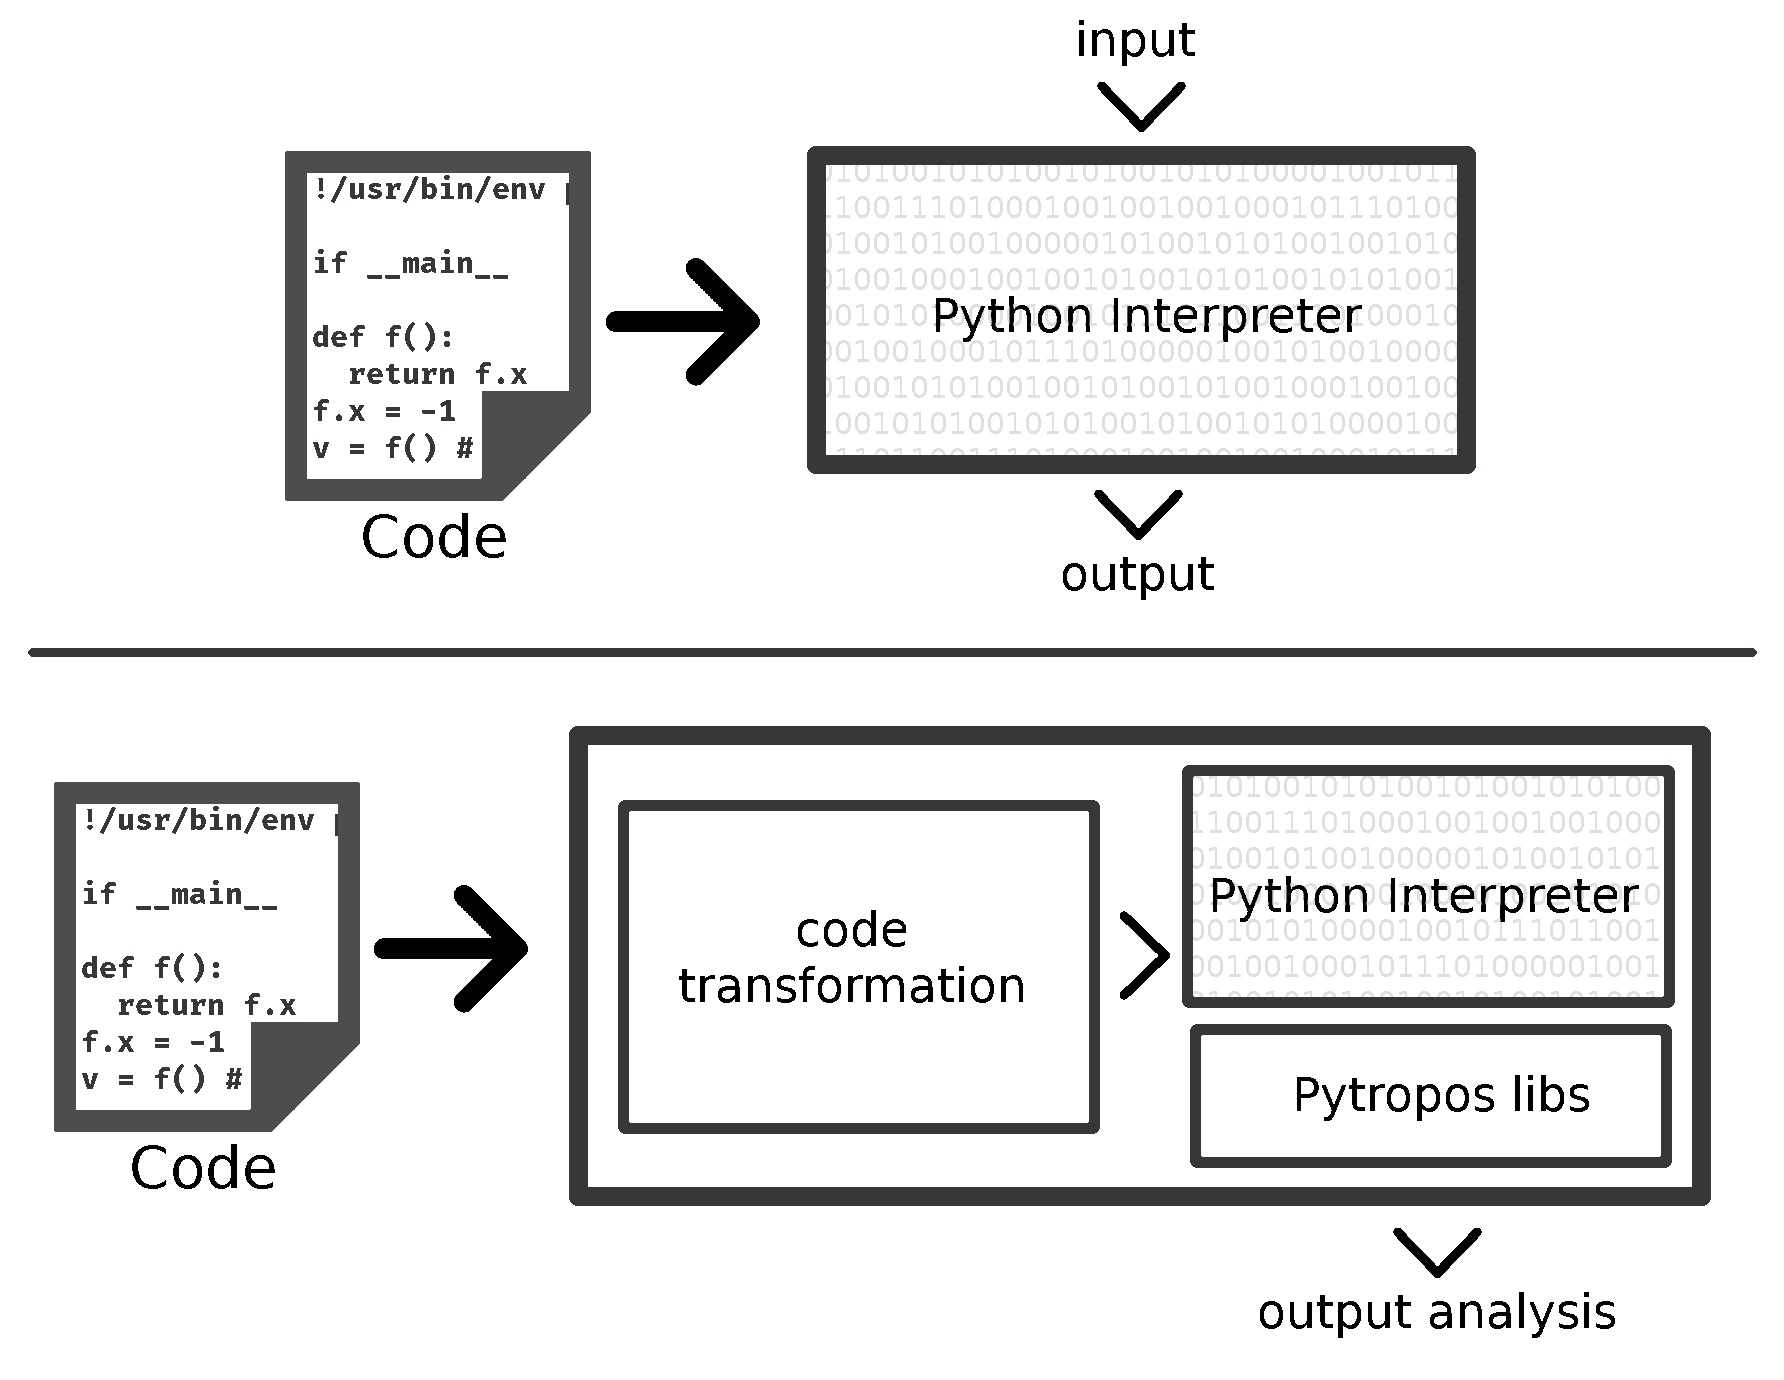
\includegraphics[width=0.6\textwidth]{figures/pytroposimage.png}
\end{center}
\caption{Up: black box step by step of executing a piece of code in Python (CPython). Down:
  Pytropos extension of Python. Pytropos transforms the code prior to run it by CPython.
  The transformation wraps the code to be run with the help of a custom library.
  \label{pytroposinter}}
\end{figure}

Pytropos works in a similar way as any other Python interpreter does. Pytropos reads code
and executes it sentence by sentence. Its main difference to CPython is that it does not
transform code into bytecode but it wraps the code before it is transformed into CPython
bytecode. The code is wrapped to use a library that implements the semantics of the
Abstract Interpreter. See Figure~\ref{pytroposinter}.

Similar to how Python works, Pytropos not only \enquote{runs} individual files but also
offers a REPL (Read-eval-print loop) to check small portions of code.

\section{Wrapped code + libs + interpreter vs.~from scratch interpreter}%
\label{wrapped-code-libs-interpreter-vs.from-scratch-interpreter}

The traditional methodology to build an interpreter is to code the parser and the
semantics of the language in one big program. For a language like Python, building an
interpreter from scratch would require considerable effort given the large amount of
characteristics Python comes with. A \enquote{complete} Python implementation would
require to implement--among other things--memory management, garbage collection, function
calling and return, dynamic type analysis, exception handling.

\textcite{ortin_towards_2015} showed how to build a Static Type Analysis by means of
rewriting the code to operate with the types of values rather than with the values
themselves, i.e.~the result of executing the code is not some values but some types. For
example, consider the following small piece of code:

\begin{pythoncode}
a = 2 + 4
b = a + "yep"  # this will fail
c = a / 2
\end{pythoncode}

Notice how even though the piece of code fails to run successfully,
we can determine the types of all variables. \pycode|a| has type
\pycode|int|, \pycode|b| has no type as it cannot be
computed, and \pycode|c| has type \pycode|float| because the
division of \pycode|int|s in Python 3 gives us back a \pycode|float|.

We can build a library that operates on types (rather than values) and
then we can rewrite the piece of code above into:

\begin{pythoncode}
import typeops as to
a = to.add(int, int)
b = to.add(a, str)
c = to.div(a, int)
\end{pythoncode}

If the library has properly defined the methods \pycode|add| and
\pycode|div|, we can be sure that the code will run without any error.
Notice that the library is able to find type mismatches by embedding
checks in the functions \pycode|add| and \pycode|div|. The library can,
effectively, perform Static Type Analysis on a piece of code.

Pytropos is implemented following the same strategy: a library that
operates over abstract values, and a transformation procedure that takes
the code and wraps it to use the library. The final step is to run the
wrapped code and collect the generated errors\footnote{%
  This strategy has been applied in the past for similar purposes, mainly to reuse
  infrastructure. It was used by \textcite{lauko_symbolic_2018} for symbolic computation
  of LLVM bytecode.
  %\inlinetodo{actually I'm not aware of any other example where this has been done :S}
  }.

The main advantage of translating code into wrapped code is the reuse of
infrastructure. One does not need to write all the infrastructure that
an interpreter needs. Pytropos does not implement its own call system,
heap management or garbage collection. All of it is managed by the
underlying Python implementation where the code is executed.

Nevertheless, this approach has three main disadvantages. First, all operations, function
calls, attribute access, subscript access and the whole Python semantics, must be coded
into the library and in the transformation function. Second, the place where any operation
has occurred must be preserved too, otherwise, it is impossible to find where an error has
occurred. Finally, all variable accesses must also be wrapped, otherwise the execution
would stop if one finds an undefined variable.  Because of all of this wrapping, the
transformation does not produce a simple, human-readable output.

To show, how currently Pytropos wraps and transforms the code consider the code below
from the piece of code above:

\begin{pythoncode}
import pytropos.internals as pt
st = pt.Store()
pt.loadBuiltinFuncs(st)
fn = 'test.py'
st[('a', ((1, 0), fn))] = pt.int(2).add(pt.int(4), pos=((1, 4), fn))
st[('b', ((2, 0), fn))] = st[('a', ((2, 4), fn))].add(pt.str('yep'), pos=((2, 4), fn))
st[('c', ((3, 0), fn))] = st[('a', ((3, 4), fn))].truediv(pt.int(2), pos=((3, 4), fn))
\end{pythoncode}

Not as nice as the first example.

Pytropos started out from the same idea as \textcite{ortin_towards_2015}
but it differs on its principal goal. Pytropos goal was not to perform
Static Type Analysis but Static Value Analysis. After working for three
months on a prototype, it became blatantly clear that trying to wrap the
code naïvely did not work very well, i.e.~the code was a hacky and not
very resilient. The library and transformation needed to be based on a
solid theoretical framework.

Enter Abstract Interpretation. Abstract Interpretation offers the ideal
framework for Static Value Analysis, it is well understood, with solid
theory and extensive work on it has been done for the last four decades.

\textcite{ortin_towards_2015} strategy alone may still be a good idea
for Static Type Analysis, but it may not work without a framework to
glue together the semantics of the language with those of the analysis.
Their legacy to Pytropos is the reuse of Python infrastructure by
wrapping the code and not building an interpreter from scratch.

\section{Assumptions}\label{assumptions}

Pytropos is limited to work only with Python 3.6 or higher. Pytropos
uses variable annotations to allow the user to specify the shape of
NumPy arrays when Pytropos is not able to \enquote{infer} their value.
Variable annotations were introduced on Python 3.6 \autocite{pep526}.

The goal of Pytropos is to warn the user when an operation will fail at runtime. It is not
a goal of Pytropos to verify the code and prove its correctness (Pytropos is not a tool
for verification).

Pytropos goal is not to replace MyPy, flake8, or any other static
analysis Python tool\footnote{I use MyPy and flake8 in every project and
  I am thankful for the years of effort put into these amazing tools.
  Thank you, guys!}. Pytropos is meant to be an aid for developers when
working with tensors.

Based on that, I present the main assumptions taken into account at the design stage of
Pytropos:

\begin{itemize}
\tightlist
\item The user wants as little warnings on the code as possible. Pytropos should warn the
  user for errors it is sure will occur at runtime.
\item The user cares only about the shape of tensors and not about their actual content.
\item If Pytropos is not able to infer the value of a variable, the user can (optionally)
  annotate the type/value of the variable. If the annotation is not more precise than the
  value that Pytropos has already inferred the inferred value will not be changed.
\end{itemize}

\section{Details about the guts}

To start with, I do not follow the structure defined in the previous chapter for how
elements are saved in memory. I did not explicitly defined a Heap (\(\Hea^\sharp\)) but
rather, I make use of Python's heap. The main reason to not define a custom Heap is the
cost associated to it, especially the definition of a Garbage Collector. The classes
\pycode|AbstractMutVal| and \pycode|Store|, the implementations of
\(\mathbf{Object}^\sharp\) and \(\Glo^\sharp\), respectively, do not point to
\(\mathbf{Addr}^\sharp\)s but they point to \pycode|PythonValue|s directly (again, because
CPython manages the heap not Pytropos). The global scope, \pycode|Store|, is an object
that takes a \pycode|str| and returns a \pycode|PythonValue|. An
\(\mathbf{Object}^\sharp\), \pycode|AbstractMutVal|, is an object that has an associated
type and operations, and it can point to any \pycode|PythonValue|.
%In this way, the Pytropos resembles more the graph representation than
%the classical Heap representation\footnote{Both representations are
%  explained in detail in the previous chapter}.

The class \pycode|PythonValue| implements the \(\mathbf{Val}^\sharp\) Abstract Domain. A
\pycode|PythonValue| is a wrapper around either an \pycode|AbstractValue| or an
\pycode|AbstractMutVal| (the implementations of \(\mathbf{PrimVal}^\sharp\) and
\(\mathbf{Object}^\sharp\)). Note that \pycode|AbstractMutVal| subclasses
\pycode|AbstractValue|, as well as do \pycode|Int|, \pycode|Float|, \pycode|NoneType| and
\pycode|Bool| which implement \(\text{Int}^\sharp\), \(\text{Float}^\sharp\),
\(\text{None}^\sharp\) and \(\text{Bool}^\sharp\), respectively.

\pycode|AbstractValue| is an abstract class that defines all the
operations supported (\pycode|+|, \pycode|*|, \ldots{}) by Pytropos, and
what it is required for a function call, subscript access and attribute
access. \pycode|AbstractValue|, in its turn, subclasses
\pycode|AbstractDomain| an abstract class that defines the methods every
Abstract Domain should have, namely \pycode|is_top()|, \pycode|join()|,
\pycode|top()| and \pycode|widen_op()|. \pycode|PythonValue| and
\pycode|Store|, unsurprisingly, also subclass \pycode|AbstractDomain|.

Figure~\ref{classPytropos} presents the class diagram showing the relationships
between the different components in Pytropos.

\begin{figure}
\begin{center}
  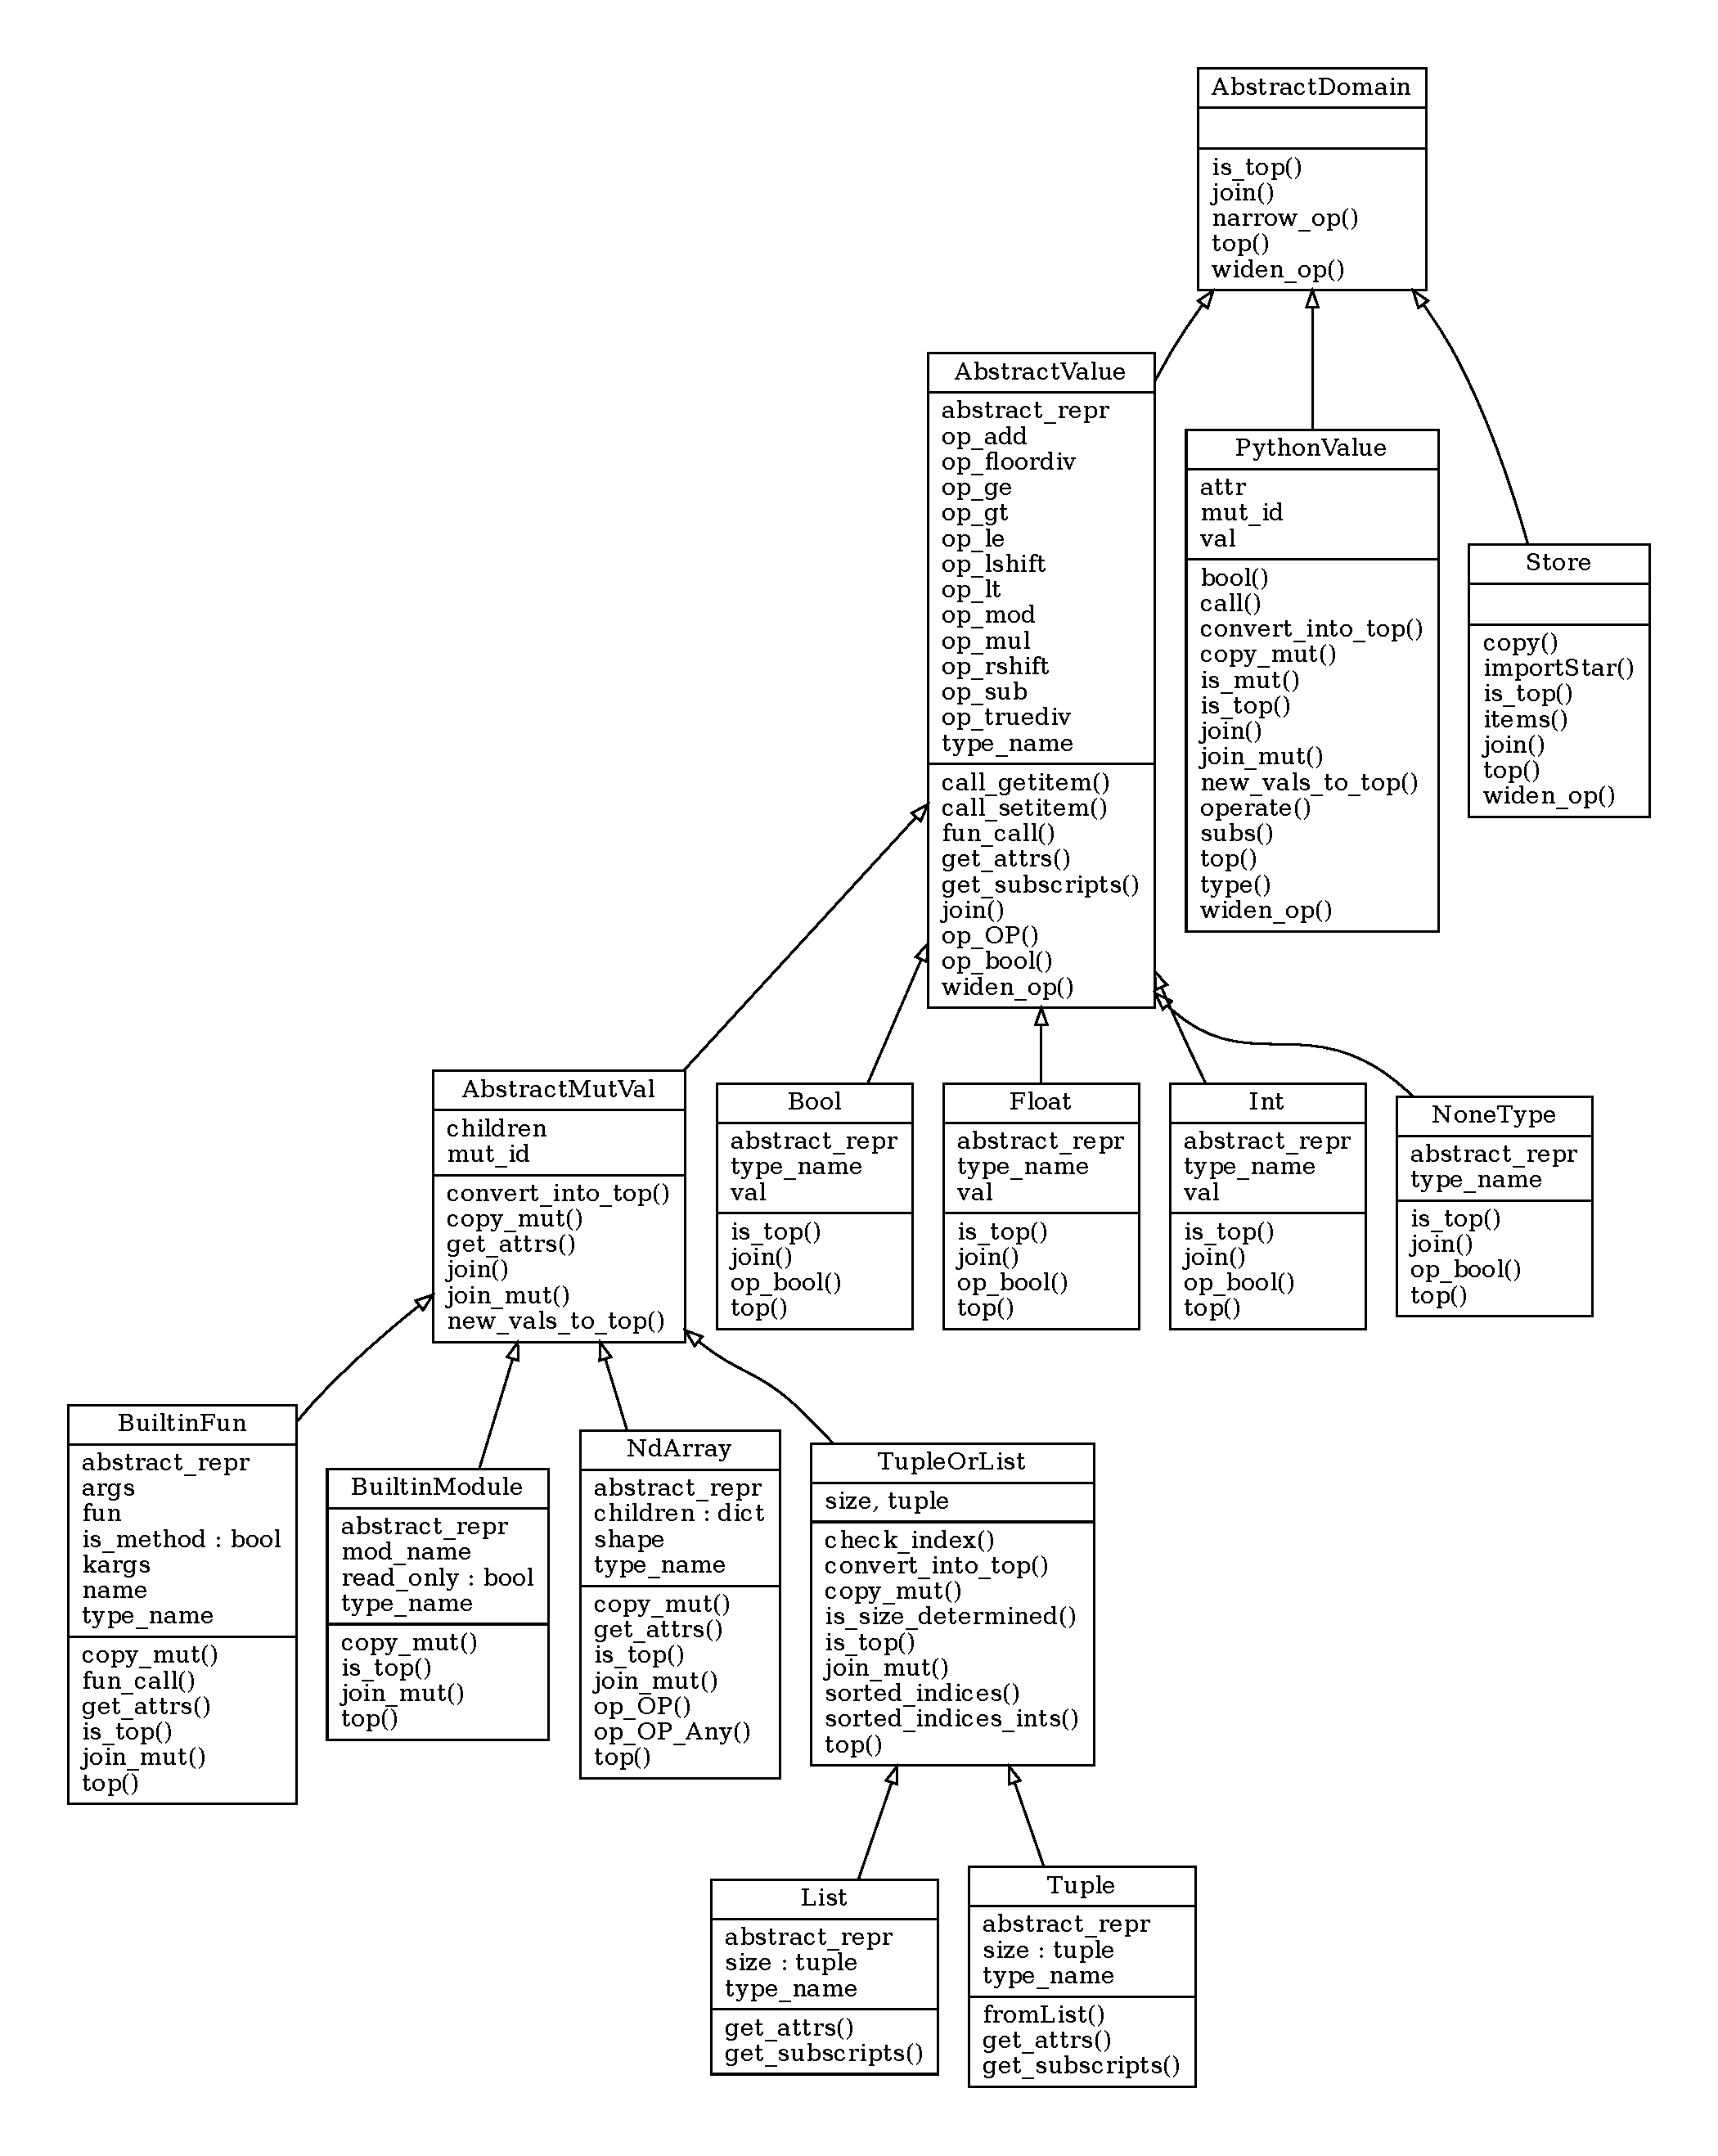
\includegraphics[width=0.95\textwidth]{figures/classes_Pytropos-small.pdf}
\end{center}
\caption{Class diagram for Pytropos, the implementation of the Abstract
  Interpreter.\label{classPytropos}}
\end{figure}

%\todo{add types to each attribute, and add hidden attributes like
%\pycode+__getitem__+}

\texttt{<prim-callable>} and all other \(\mathbf{Object}^\sharp\)s are implemented by a
subclass of \pycode|AbstractMutVal|: \texttt{<prim-callable>} by \pycode|BuiltinFun|,
\texttt{Module} objects by \pycode|BuiltinModule|, \pycode|list|s by \texttt{List}, and
\pycode|tuple| by \texttt{Tuple}.

The implementation of the Abstract Interpreter also includes a class log that stores all
warnings generated in the abstract interpretation of the code.

% \inlinetodo{mention that \texttt{children} is the function \texttt{Key\ -\textgreater{}\
%     Addr\ +\ Undefined}}
% \inlinetodo{mention that \texttt{joinVal} is defined as \texttt{join\_mut} in
%   \texttt{PythonValue}, and \texttt{joinObject} is defined as \texttt{join\_mut} in
%   \texttt{AbstractMutVal}}


\chapter{Validation and Discussion}\label{validation-and-discussion}

{\ichange{This is just a DRAFT! REVISE!!}}

So, this chapter is about which kind of tests where performed and which
were considered but didn't cut it. The Python Regression tests are very
broad in scope, they use too many builtin capabilities which makes it
hard for a prototype like Pytropos to make any of them work (and that is
maybe why they are the regression tests for Python, after all they need
to check as many characteristics as possible!).

\section{Validation}\label{validation}

{\inlinetodo{Over which set of problems you tested your code. The
problems are pieces of code written by me on my own and other collected
from programs from the internet}}

I created two types of tests: unit regression tests and property-based
tests. The unit tests let us check for any kind of anomalous behaviour
while property-based tests ensure that the abstraction follows the
Python implementation that underlies.

Comparing against the official regression tests is left for future work,
as the number of builtin characteristics does not yet reach a
satisfactory level to check.

\subsection{Unit Tests}\label{unit-tests}

There are a total of 79 unit tests checking various parts of the
Abstract Interpreter. The tests can be categorised into:

\begin{itemize}
\tightlist
\item
  binary operations
\item
  type annotations
\item
  numpy library
\item
  if branching
\item
  while looping
\item
  lists and tuples
\item
  join stores
\end{itemize}

In the table below the result of executing all tests can be seen. The
coverage is not 100\% as Pytropos is still in development. The tests
check not only for what Pytropos is able to do now, but what it should
be able given the description of it given in the document.

\begin{verbatim}
Category     Total lines    Tests     Time analysing   covered  non-covered   Total coverage
Binary ops   120            10        500ms            8        2             80%
\end{verbatim}

\subsection{Property-based Tests}\label{property-based-tests}

Property-based tests that try to disprove a property. For example, a
property of lists is that anytime you add a new element to a list of
size \pycode|n| you will get a list with size \pycode|n+1|. I use
property-based tests to check for correcness of Pytropos against Python
on builtin operations for builtin values.

There are a total of 20 of such tests. Because each one of them is a
property-based tests, they are tested against a 100 values that try to
disprove the property. This kind of testing proved to be extremely
helpful at the start of the development, as the \enquote{property-based
tester} was able to find numerous counter examples to the properties.
Python throws an exception on many cases of bad values, the
\enquote{tester} was able to reliably (at least at the start) to come up
with combinations of values that would go wrong when operated. Some of
the most honorable mentions are:

\begin{itemize}
\tightlist
\item
  Zero-division error on expressions like \pycode|5 \% 0| or
  \pycode|5 \% False|
\item
  Value error on expressions like \pycode|5 << -2|
\item
  Excesive High-memory consumption on expressions like
  \pycode|5 << 10**10|
\item
  Overflow error on expressions like \pycode|10**209 + 2.0|
\end{itemize}

\section{Discussion}\label{discussion}

\inlinetodo{add many, many examples of what the program is able to catch and  what not,
based on the errors above}

\inlinetodo{explain and add a picture of what Pytropos shows when executed}

%--

Pytropos is still in a very young age. It is not able to check many,
many characteristics present in Python code (some of the biggest
culprits are \pycode|for| statement, custom classes and objects,
exception handling and the lack of builtin definitions), but when code
is given to it that it can actually check.

Pytropos is able to check for the many common cases and mistakes that
can be made when working with tensors. It is able to calculate the shape
of tensors in a variety of circumstances (NumPy's \pycode|array| can
evaluate almost anything as an array, therefore detecting the shape of
any value passed to \pycode|array| is an accomplishment in itself. An
example of why this is important can be seen in the library{\todo{add
ref to numpy mypy lib}}, where they define a stub for mypy to check of
the library numpy, and what they do in the case of \pycode|array| is
basically give up).


\chapter{Related Work}\label{related-work}

A big, widely used, and mature language like Python has no lack of Static Analysis tools.
A big, widely used, and mature area like Machine Learning has no lack of people trying to
build tools to make writing code for them easier. In this chapter, a brief overview of the
many Static Analysis tools developed for Python code and the several approaches taken to
solve the problem of tensor shapes are given.

\section{Static Analysis in Python}

% {\inlinetodo{add note in the difficulty of knowing what is the theory
% behind some of the most widely used linters}}

In Table~\ref{relatedworktable}, a list of all analysis tools found in the literature
and libraries is given. The usage of a tool refers to how is the tool used by developers:
embedded in the python interpreter, used as a linter, or as a library that runs with the
code to analyse. The Analysis base of a tool refers to which is the theory behind the
tool, how it works underneath.
% The purpose of analysis tools are varied and broad in scope.

\begin{sidewaystable}[p]
\centering
\begin{threeparttable}
\begin{longtable}[]{|l|l|l|l|}
  \caption{Analysis tools for Python.
  }\label{relatedworktable}\tabularnewline
  \toprule
  Tool Name / Source & Usage & Analysis base & Purpose \tabularnewline
  \midrule
  \endhead
    \textcite{cannon_localized_2005}                     & Embeded & Type analysis           & Typecheking     \tabularnewline
    Pep8\tnote{0}                                        & Linter  & N/A                     & Code style analysis \tabularnewline
    Pyflakes\tnote{1}                                    & Linter  & N/A                     & Various checks  \tabularnewline
    Pylint \autocite{thenaultpylint}                     & Linter  & N/A                     & Various checks  \tabularnewline
    PyChecker \autocite{norwitzpychecker}                & Linter  & N/A                     & Various checks  \tabularnewline
    MyPy \autocite{lehtosalo2016mypy}                    & Linter  & Gradual Type Analysis   & Type checking   \tabularnewline
    Enforce\tnote{2}\tnote{+} (defunct)                  & Library & Gradual Type Analysis   & Type checking               \tabularnewline
    Sagitta\tnote{3}\tnote{+} (defunct)                  & Library & Type analysis           & Type checking               \tabularnewline
    StyPy \autocite{ortin_towards_2015}                  & Linter  & Novel                   & Type checking               \tabularnewline
    Lyra\tnote{4}                                        & Library & Abstract Interpretation & Various analyses (including Value Analysis) \tabularnewline
    Pytropos\tnote{5} (This Work)                        & Linter  & Abstract Interpretation & Value Analysis (specialised on tensor shapes) \tabularnewline
    PyType\tnote{6}                                      & Linter  & N/A                     & Type checking and inference \tabularnewline
    ICBD\tnote{7} (defunct)                              & Linter  & N/A                     & Type checking and inference \tabularnewline
    Pyre\tnote{8}                                        & Linter  & Abstract Interpretation & Type checking               \tabularnewline
    Nagini\tnote{9} \autocite{eilers_nagini_2018}        & Linter  & SMT (Viper)             & Verifier                    \tabularnewline
    Typpete\tnote{10} \autocite{hassan_maxsmt-based_2018} & Library & SMT                     & Type inference              \tabularnewline
    \textcite{fromherz_static_2018}\tnote{*}             & N/A     & Abstract Interpretation & Value Analysis | Verifier   \tabularnewline
    \textcite{monat_static_2018}\tnote{*}                & N/A     & Abstract Interpretation & Type Analysis               \tabularnewline
    PyAnnotate\tnote{+}\tnote{11}                        & Library & Gradual Type Analysis   & Type inference              \tabularnewline
    MonkeyType\tnote{+}\tnote{12}                        & Library & Gradual Type Analysis   & Type inference              \tabularnewline
  \bottomrule
\end{longtable}
\begin{tablenotes}
  \item[+] \footnotesize It is not an static analysis. It is a dynamic analysis.
  \item[*] Tool has not been made public.
  \item[0] Homepage: \url{https://pep8.readthedocs.io/}
  \item[1] Homepage: \url{https://pypi.org/project/pyflakes/}
  \item[2] Homepage: \url{https://github.com/RussBaz/enforce}
  \item[3] Homepage: \url{https://github.com/peterhil/sagitta}
  \item[4] Homepage: \url{https://github.com/caterinaurban/Lyra}
  \item[5] Homepage: \url{https://github.com/helq/pytropos}
  \item[6] Homepage: \url{https://github.com/google/pytype}
  \item[7] Homepage: \url{https://github.com/kmod/icbd}
  \item[8] Homepage: \url{https://github.com/facebook/pyre-check}
  \item[9] Homepage: \url{https://github.com/marcoeilers/nagini}
  \item[10] Homepage: \url{https://github.com/caterinaurban/Typpete}
  \item[11] Homepage: \url{https://github.com/dropbox/pyannotate}
  \item[12] Homepage: \url{https://github.com/Instagram/MonkeyType}
\end{tablenotes}
\end{threeparttable}
\end{sidewaystable}

\textcite{cannon_localized_2005} was the first (to our knowledge) to try to statically
infer and type check code in Python. His idea was to infer variables' types before
executing the code and use this knowledge to speed up the execution. He acknowledged that
the nature of Python makes type inference to be too weak. Thus, the complexity that the
project brought did not improve performance in equal measure and his work was never added
to Python. This work was prior to \textcite{siek_gradual_2006} with Gradual Types, where the
developer can help the type checking algorithm to find and assert better types.

The goal of all linters is to aid the developer by flagging code as faulty. What means for a
piece of code to be faulty varies from tool to tool. Pep8 checks for syntactic deviations
of the style guide, Pep 8\footnote{\url{https://www.python.org/dev/peps/pep-0008/}}.
Pyflakes, Pylint and PyChecker define a variety of checks for common scenarios where a
piece of code is known to fail, e.g.~undefined variables. MyPy, PyType and Pyre focus on
type checking optionally, type-annotated code. Nagini focuses on verifying pieces of Python
code using the mature Viper \autocite{muller_viper_2016} infrastructure. Pytropos
objective is different from all the other available linters: Value Analysis.

Our work is closest to \textcite{fromherz_static_2018} as they focus on Value Analysis as
well. Fromherz et.~al focus is on building an Abstract Interpreter to verify Python code.
Our focus is not in verification but in the shape of Tensors. Their Abstract Interpreter
incorporates more capabilities than we do: exception handling and support for breaking
flow instructions. Unfortunately, they have not yet made their implementation public.

\section{Tensor Shape Analysis}

% {\inlinetodo{add idea from http://nlp.seas.harvard.edu/NamedTensor
% Alexander, who suggests building the libraries in a different way so we
% do not have some of the problems of working with nameless shapes}}
%
% {\inlinetodo{extend solutions described below with the new libraries you
% found, comment below}}
%  {2018.06.25} tensors papers and libraries
%  * (mypy-python) https://github.com/machinalis/mypy-data/tree/master/numpy-mypy
%  * (python (in java)) ariadne https://github.com/wala/ML (paper by dolby (weird name))
%  * (haskell) https://github.com/achirkin/easytensor
%  * (nopython) https://github.com/Diderot-Language/diderot (Diderot: a domain-specific language for portable parallel scientific visualization and image analysis)
%                                                           Chiw et al (2018) - Compiling Diderot
% \inlinetodo{there was one more paper to take into account. I don't recall its name but
% it was about a tool to check for the shape of tensors!!}

\subsection{Solutions in other languages}

We may think that if a type system is not expressive enough to capture the
shape of tensors, then we should just start writing code in a language
which does. We may write code in a language like Haskell or even C++,
which have very strong and expressive type systems (it is possible in
C++ to enforce the shape of the tensors with the use of templates and
constraints (C++20)).

In fact, solutions in other languages exist. For example,
\textcite{chen_typesafe_2017} type checks the shape of tensors
(operations) by restricting what can be constructed (via constraints in
the types of objects and functions). Chen's solution uses the powerful
type system of Scala (which runs over the JVM).
\textcite{eaton_statically_2006} does the same, although in an old
version of Haskell. Eaton's encoding of tensor shapes is awkward because
Haskell did not have, at the time, support for natural numbers at the
type level. Haskell also lacked on syntactic sugar for type functions.
\textcite{abe_simple_2015} implement type checking for matrices (aka,
tensors) in OCaml. The library detects the shape of the matrices at
compile time. \textcite{rakic_statically_2012} type check tensor shapes
(they call them matrices) with templates in C++. Templates are only
accessible at compile time, thus the Rakić et al.~library type checks at
compile.

One recent effort to type check tensor shapes in Haskell is the library
\pycode|tensorflow-haskell-deptyped| written by
\textcite{elkin_haskell_2018}. The library is written as a wrapper
around the library port of TensorFlow for Haskell.
\pycode|tensorflow-haskell-deptyped| enforces at the type level how and
which results an operation between compatible tensors are to be performed.

A different path, not yet explored, is to extend an existing type checking system, like
MyPy, and extend it with dependent types. Dependent types allow us to carry information
from the term level to the type level, i.e.~we can encode information of our data
(available only at runtime) into the type system. Over this extended type system, we could
implement some restrictions to the operations applied to different types (this is, in
fact, the strategy taken in the library tensorflow-haskell-deptyped).

\subsection{Theoretical Solutions}\label{theoretical-solutions}

The problem of mismatched shapes is not new, in fact, it is so common
that it has appeared several times with similar solutions
\autocites{arnold_specifying_2010}{griffioen_type_2015}{rink_modeling_2018}{slepak_array-oriented_2014}{trojahner_dependently_2009}.
All solutions, though, are theoretical, they propose type systems which,
if they were to be implemented, could warranty type safety, i.e.~no
mismatching of tensor shapes could ever happen at runtime.

The following is a small discussion about the different solutions
proposed to type check tensors found in the literature\footnote{As a
  side note, it is interesting to notice how difficult is to communicate
  ideas in science. All the papers presented in this section hope to
  solve the same (or similar) problem, but they do not reference each
  other, which means that none of them knew what the others were doing.
  The principal reason for this, I think, it is because they all called
  the problem differently.}:

\begin{itemize}
\item
  \textcite{trojahner_dependently_2009}: A paper on type checking of
  arrays. They define all type restrictions using dependent types
  (something that no other paper does). The special keyword of this work
  is \enquote{array programming}.
\item
  \textcite{arnold_specifying_2010}: A paper focused on type checking of
  sparse \enquote{matrix} operations. They define a functional language
  that can be translated into a lower level language or machine code.
  They give a complete formalization of the algorithms and proofs of
  correctness in Isabelle. The special keyword of this work is
  \enquote{sparse matrix}.
\item
  \textcite{griffioen_type_2015}: A paper focused on type checking and
  inference of arrays in array programming and vector spaces. They
  define a special type system in which tensors are first class
  citizens. The algorithm used for type checking is
  \enquote{Unification} which allows them to infer the type shape of
  arrays. The special keyword of this work is \enquote{array
  programming}.
\item
  \textcite{slepak_array-oriented_2014}: A paper that tries to formalise
  array-oriented programming languages and extend them with unit-aware
  operations. Array-oriented programming languages are languages which
  base all their computations in arrays (like Matlab), but they usually
  aren't formalised. The types of arrays not only carry information
  about their shape but also of the unit they carry. The special
  keywords of this work are \enquote{array-oriented programming} and
  \enquote{unit-aware computation}.
\item
  \textcite{rink_modeling_2018}: In this paper, Rink formalises a type
  system to type check the shape of tensors and defines a language to
  use with the type system. It is a custom type system which does not
  require dependent types. The special keyword of this work is
  \enquote{tensor manipulation language}.
\end{itemize}


\chapter{Conclusions and Future Work}\label{conclusions}

\section{Conclusions}

In this work, we have presented the definition and implementation of an Abstract
Interpreter for Python focused on the analysis of tensor shapes.

We showed how can Abstract Interpretation be applied to a dynamically typed programming
language like Python with the goal of defining a Static Value Analysis. To make this
possible, first, we specified small-step (concrete) semantics for Python taking into
account Python dynamically typed variables and aliasing. To build the Abstract Interpreter
we defined an apt Abstract Domain for all values in the language, an Abstract Domain for a
state of a program with aliasing, and abstract semantics. Our approach to build the
Abstract Interpreter is easily extendable to check for more than built-in values as we
showed by extending the syntax and semantics of Python to handle the shape of NumPy arrays
(tensors). The Abstract Interpreter is able to use type annotations from the user to get
more precision on the values it is able to analyse.

We presented a working implementation of the Abstract Interpreter, Pytropos, which is able
to analyse the shape of tensors in a variety of scenarios. The interpreter can work as a
linter for IDEs catching potential errors as the developer codes.

In brief, the work done includes:

\begin{itemize}
\tightlist
\item A specification of a subset of Python 3.6 (Syntax and small-step semantics).
\item An Abstract Domain for Python Values.
\item An Abstract Domain for Python program states.
\item The semantics of an Abstract Interpreter for Python.
\item The implementation of the Abstract Interpreter, Pytropos\footnote{Available at:
    \url{https://github.com/helq/pytropos}}.
\item An application for the Abstract Interpreter to statically analyse the shapes of
  tensors and tensor operations.
\item A series of tests showcasing the abilities of the Abstract Interpreter and its
  failures.
\item A way for developers to annotate code to improve the accuracy of the Abstract
  Interpreter.
\end{itemize}

The presented Python formalisation is easily extendible to calculate the value of a
library-defined class. NumPy arrays were added to the formalisation to show how to analyse
code the shape of tensors.

%The State Abstract Domain is wholy defined by the join operation.
%An Abstract Domain for the state of the program was designed. The Abstract Domain was
%built to take into account aliasing. If there is some inconsistency between two states
%between two states are collapsed into a $\top$ value. $\top$ values can be think of as
%\verb|?| types in Gradual Type systems.

The abstract semantics, the semantics of the Abstract Interpreter, are easy to develop. It
was shown how to get from the concrete semantics (small-step semantics) to the abstract
semantics.

Testing showed that the Pytropos, the implementation of the Abstract Interpreter, is able
to check many common shape mismatches. The biggest problem of the implementation
is on the lack of support for built-in functions and values.

When the Abstract Interpreter cannot compute the correct tensor shape, the user may help
the Abstract Interpreter with Type Annotations. If the user gives a type annotation that
does not improve the precision of the computed value, the interpreter will warn the user
of his mistake.

\section{Future Work}\label{future-work}

Python is a huge and rich language. The amount of characteristics that Python has exceeds
by far what a single human can implement in the span of a master thesis.

Much work is left to improve Pytropos so that it can be used by the regular developer. We
propose the following roadmap to continue building the Abstract Interpreter:

%\inlinetodo{Defining an abstract interpreter for sets}

\begin{itemize}
\tightlist
\item Extend Pytropos to include Exception handling. A similar approach to that of
  \textcite{fromherz_static_2018} could be a good starting point.
\item Improve how copying and \textbf{join}ing stores (states of the program) are done.
  The join operation between stores is very, very costly. Walking through the graphs
  becomes prohibitively expensive as the program to analyse grows in number of \pycode|if|
  and \pycode|while| sentences. This associated cost could be reduced if only
  \enquote{diff}s of stores were used. One way to do this is by using immutable
  structures for all values in the implementation. Using immutable structures would
  require the explicit implementation of the heap and garbage collector.
\item Extend Pytropos to handle breaking control statements (\pycode|continue|,
  \pycode|break| and \pycode|return|). \textcite{fromherz_static_2018} also present a way
  to handle breaking control statement in Python.
\item Extend the global scope to handle local and non-local scopes. The scope rules of
  Python are mildly complex with four different variable scopes: global, local, nonlocal,
  and class. Something to take into account is the ability of CPython to statically
  analyse the use of local and non-local variables before interpreting the code.
\item Extend \(\mathbf{Val}^\sharp\) with user-defined functions and objects. Once the
  interpreter handles user-defined functions properly, extending the interpreter to work
  with user-defined objects is not a big problem. The biggest difficulty with
  objects is implementing the MRO rules in charge of how to inheritance work in Python.
\end{itemize}

% \inlinetodo{add idea that Pytropos could be run inside an IDE just as paper: Sulir Poruban
%   (2018) - Augmenting Source Code Lines with Sample Variable Values}
% \inlinetodo{add idea that the parser could be extended to add holes, or insert Top values,
%   just as done in paper: Omar et al (2018) - Live Functional Programming with Typed Holes
%   (I wrote something about it in the SoRI)}
% \inlinetodo{The Python Regression tests are very broad in scope, they use too many builtin
%   capabilities which makes it hard for a prototype like Pytropos to make any of them work
%   (and that is maybe why they are the regression tests for Python, after all they need to
%   check as many characteristics as possible!).}

Besides what is left to do to make Pytropos more powerful, there are some tasks related to
the formality of the work. This work presented some concrete and abstract semantics for
Python but there was never a proof of their correctness. We consider the following to be the
problems to solve to prove the formalisation correct:

\begin{itemize}
\tightlist
\item Give a complete and through formal definition for a subset of Python in a
  proof-assistant language such as Agda, Idris, Coq, and Isabelle/HOL.
\item Define in the same proof-assistance language the Abstract Domain, the properties it
  must follow, and the abstract semantics.
\item Prove that the abstract semantics are in fact consistent with the concrete semantics
  and abstract domain.
\end{itemize}

% Such a formalisation of Python would likely/hopefully help future
% endeavours on proofs and verification.

% Notice that any formalisation of Python must take some stance on how closely it wants to
% follow the implementation of CPython. CPython has many, many little undocumented semantic
% subtleties. Trying to write a full formal definition of Python semantics is probably
% undoable.


%----------------------------------------------------------------------------------------
% THESIS CONTENT - APPENDICES
%----------------------------------------------------------------------------------------

\appendix % Cue to tell LaTeX that the following "chapters" are Appendices

% Include the appendices of the thesis as separate files from the Appendices folder
% Uncomment the lines as you write the Appendices

\chapter{Python Static Analysis based on Abstract Interpretation}%
\label{appendix-ai-theory}

This appendix is divided into two parts: first, we present a reduced set of the Python
syntax together with a (partial) operational semantics; second, we show the use of the
formal semantic definition to define the abstract interpretation solution we implemented.

This chapter is meant to explain the theory behind the Abstract Interpreter implemented.
In Chapter~\ref{pytropos-analysis-implementation} an explanation on the implementation
details is given.

\section{Python (reduced) syntax and semantics}

Python has no official small-step (formal) semantics. The Python Software Foundation
defines a Reference Manual for the language
\autocite{python_software_foundation_python_2019}, but they are explicit that the manual
does not define a full specification for the language. Quote: \enquote{\ldots{} if you
were coming from Mars and tried to re-implement Python from this document alone, you might
have to guess things and in fact, you would probably end up implementing quite a different
language.}

There have been a couple of small-step semantics defined for Python
\autocites{politz_python_2013}{fromherz_static_2018}{guth_formal_2013}{ranson_semantics_2008}.
In this work, we define yet one more time small-step semantics for Python. We decided to
define our small-step semantics for Python because of our specific needs.

Our semantics definition resembles the most that of \textcite{fromherz_static_2018}. In
fact, our
definition is loosely based on \textcite{fromherz_static_2018}. As Fromherzet.~al, we
define each expression and statement step as a function from states to states of the
program, but opposed to them we do not include exception handling and breaking statements.
Our definition allows every single value in the language to be an object: functions,
attributes, subscripts, and primitive values are all objects just as in regular Python.
The following is valid in Python and in our definition:

\begin{pythoncode}
a = []
b = a.append
b(3)
a.append(2.0)
print(a)  # prints: [3, 2.0]
\end{pythoncode}

In this sense, our definition is closer to that of \textcite{politz_python_2013}, where
they also show how their semantics are able to handle similarly complex examples.

\subsection{(Reduced) Syntax}\label{reduced-syntax}

A simplified version of Python's Syntax. Modified from AST's syntax below.

% {\inlinetodo{Translate into LaTeX equations}}

\begin{verbatim}
mod = stmt*  -- A program. Starting point

expr = Int(i) for i \in \N | Float(j) for j \in floats
     | True | False | None

     | identifier         -- variable name

     | expr op expr       -- eg, a + 5
     | expr cmpop expr    -- eg, a < 5
     | expr(expr*)        -- Function calling

     | expr.identifier    -- Attribute access
     | expr[expr]         -- Not supported for NumPy Arrays :S
     | [expr*]            -- list
     | (expr*)            -- tuple

stmt = del expr           -- delete expression
      | expr = expr       -- assignment
      | expr op= expr     -- augmented assignment
      | expr: expr = expr -- type annotation
      | while expr: stmt+
      | if expr: stmt+
      | import alias+
      | from identifier import alias+
      | expr              -- An expression can be an statement

op = + | - | * | / | % | ** | << | >> | //
cmpop = < | <= | > | >=

alias = identifier | identifier as identifier

identifier = string  -- with some restrictions
\end{verbatim}

The syntax above is a subset of the Python 3.6 syntax. CPython does not directly interpret
code written in the syntax above. The usual steps of lexing and parsing into a more
explicit representation are necessary. We will define the semantics of the language over a
reduced parser syntax and not the aforementioned syntax. The reasoning behind it is that
in this syntax it is easier to indicate the context in which an expression is being
executed. \footnote{Modified from the Python 3.6 syntax found at
\url{https://github.com/python/typed_ast/blob/89242344f18f94dc109823c0732325033264e22b/ast3/Parser/Python.asdl}}

\begin{verbatim}
mod = Module(stmt* body)

expr = Int(n)
     | Float(n) | True | False | None
     | Name(identifier, expr_context)
     | BinOp(operator, expr, expr)
     | Compare(expr, cmpop, expr)
     | Call(expr, expr*)
     | Attribute(expr, identifier)
     -- No need for expr_context because no user made objects are allowed yet, thus
     -- modifying attributes is not necessary
     -- | Attribute(expr, identifier, expr_context)
     | Subscript(expr, expr, expr_context)  -- No arbitrary slice allowed yet
     | List(expr*)
     | Tuple(expr*) -- No expr_context for Tuple as `(a, b) = 1, 2` is not supported

stmt = Delete(expr+)
      | Assign(expr, expr)                -- a = 3
      | AugAssign(expr, operator, expr)   -- a += 3
      | AnnAssign(expr, expr, expr)       -- a: int = 3

      | While(expr, stmt+)
      | If(expr, stmt+, stmt*)

      | Import(alias+ names)
      | ImportFrom(identifier, alias+)

      | Expr(expr)

-- Indicates why are we looking up a variable, attribute or subscript
expr_context = Load | Store | Del

operator = Add | Sub | Mult | Div | Mod | Pow | LShift
             | RShift | FloorDiv

cmpop = Lt | LtE | Gt | GtE

-- import name with optional 'as' alias.
alias = (identifier, identifier?)
\end{verbatim}

Code written in our subset of Python gets translated into this (AST) representation, over
which we define the semantics of the language. We will no describe the process of
translation (parsing), but we will explore some examples to show why the translation aids
into the definition of the small-step semantics:

\begin{itemize}
\item
  \pycode|a + b| gets translated into
  \pycode|BinOp(Add, Name(a, Load), Name(b, Load))|. Notice the
  \pycode|Load| context, it indicates that we want to get the value of
  the variable, not a reference to it (if we wanted to alter it).
\item
  \pycode|a = 3| gets translated into
  \pycode|Assign(Name(a, Store), Int(3))|. Notice the \pycode|Store|
  context, it tells us that we will get a reference to where the value
  is stored and not its value.
\item
  \pycode|del a| gets translated into \pycode|Delete(Name(a, Del))|.
  Notice the \pycode|Del| context, it tells us that we will get the
  object where it was called from as well as its position in the heap.
\item
  \pycode|a.b[3] + b.c| gets translated into

\begin{pythoncode}
BinOp(Add,
  Subscript(Attribute(Name(a, Load), b), Int(3), Load),
  Attribute(Name(b, Load), c)
)
\end{pythoncode}
\item
  \pycode|a.b[3] = 3| gets translated into

\begin{pythoncode}
Assign(
  Subscript(Attribute(Name(a, Load), b), Int(3), Store),
  Int(3)
)
\end{pythoncode}

  Notice how we only get the \pycode|Store| context for the subscript
  and not for anything else, as we only want to know where the value of
  the subscript is stored and nothing else.
\item
  \pycode|del a.b[3]| gets translated into

\begin{pythoncode}
Delete(
  Subscript(Attribute(Name(a, Load), b), Int(3), Del)
)
\end{pythoncode}

  Notice how we only get the \pycode|Del| context for the subscript and
  not for anything else, as we only want where and who belongs to the
  subscript and nothing else.
\end{itemize}

The semantics of a \pycode|del| require us
to know where the identifier or attribute is located (in an object or
the store). Assigning a variable requires us to know where to put a
variable. Accessing to inexistent attribute
(\pycode|class A(): ...; a = A(); a.length # error: attribute unknown|)
it's not the same as to defining a new attribute
(\pycode|class A(): ...; a = A(); a.length = 3 # works!|),
thus we need a way to distinguish between this three different
statement-dependent expressions.

Our subset of Python does not have the ability to allow the definition of custom functions
or classes. Despite the inability to define a custom function or class in the language, we
want to be able to call a function and access to objects attributes. We have found that
even though the amount of characteristics we support right now is small, we are able to
capture some common errors caused when coding (e.g.~\pycode|5 \% 0| fails and we can
capture it).

\subsection{Python (reduced) small step semantics}

There are two types of values (objects):

\begin{itemize}
\tightlist
\item
  Primitive values (\pycode|PrimVal|): integers (\pycode|int|s),
  Floating point numbers (\pycode|float|s), Boolean values
  (\pycode|True| and \pycode|False|), and the lonely \pycode|None|
  value.
\item
  Mutable values: \pycode|Object|. A \pycode|Object| is a value that
  holds a type, an address to where is located, and a
  \enquote{dictionary} pointing to other values.
\end{itemize}

Lists, Tuples, built-in Functions, built-in Modules, built-in Classes, and
built-in Methods derive from \pycode|Object|. Mutable Values may not
allow changing the value of their attributes, as in the case with
Tuples. The name \enquote{Mutable Values} refers to their ability to
point at other values (either Primitive and Mutable) and possibly change
them.

The \textbf{state of a Python program}--called the store of the program--is a tuple
\pycode|(Global, Heap)| where \pycode|Global| is the \enquote{global scope} of variables,
and \pycode|Heap| the heap (where all values are stored). Notice that we are ignoring the
statements to execute in the state of the program.

Putting all together we get:

\begin{verbatim}
Global = Iden -> Addr + Undefined -- Global scope
Heap = Addr -> Val + Undefined   -- Heap

Key = Iden + (string x (Iden + PrimVal))
Type = List | Tuple | Module

PrimVal = Int | Float | True | False | None
Object = Type x Addr x (Key -> Addr + Undefined)
Val = PrimVal | Object | <prim-callable>

<prim-callable> = <prim-append> | <prim-+-int> | <prim-+-float> | <prim-*-int> | ...
\end{verbatim}

A \pycode|<prim-callable>| is a value that is
a built-in function in Python. The special value \pycode|Undefined| is used
to signal unassigned values in \pycode|Heap|. If one tries to operate
with a \pycode|Undefined| value the execution should halt, operating
with \pycode|Undefined| values is forbidden as they never appear on
Python. In Python, a \pycode|Undefined| value is an erroneous memory
value or an unassigned region of memory.

A \pycode|Iden| is a Python identifier. A Python identifier is a string
that can only contain letters, numbers, and the character \pycode|_|.
An identifier cannot start with a number\footnote{We are simplifying here
  for the sake of brevity. In fact, Python 3 does allow a wide array of
  Unicode characters to construct an identifier.
  https://docs.python.org/3/reference/lexical\_analysis.html\#identifiers}.

Notice how the index (\pycode|Key|) for the function that relates a
\pycode|Object| to its attributes can be one of two things. \pycode|Key|
is either a \pycode|Iden| or a tuple \pycode|string x PrimVal|. The
idea behind indexing an object with two separate kinds of keys is to be
able to differentiate between a value that is inherent to the
\pycode|Object| and others that the object simply points. Consider a
list, an inherent, unmodifiable, value of a list is its size. The size of
a list can only be modified if an element is added or removed from it.
Now, consider the value at the index 2 of the list
\pycode|[2, 54, [True], 6, 0.0]|, the value is another
\pycode|Object|. Any object stored in a list is not an intrinsic property
of the list.

A \pycode|Key| can be a tuple \pycode|string x PrimVal|. There are
only two types of tuples in the current specification, either
\pycode|('index', val)| or
\pycode|('attr', val)|. A key of the
form \pycode|('attr', val)| indicates
us that \pycode|val| (hopefully an \pycode|Iden|) is an attribute of the
object. \pycode|('index', val)| is
used for lists.

For example, the list \pycode|[None, 4, ()]| can be expressed as:

\begin{verbatim}
(List,
 0,
 { 'size': 1,
   ('index', 0): 2,
   ('index', 1): 3,
   ('index', 2): 4
 }
),
\end{verbatim}

The first element of the triple is \pycode|List|, indicating us that the
\pycode|Object| is a list. The second element is the address on the
heap, a natural number. The third element is a function from
\pycode|Key| values to \pycode|Val|s. Strictly speaking an
\pycode|Object| cannot be defined isolated, it requires to be defined as
part of a \pycode|Heap|:

\begin{verbatim}
H = {
  0: (List, 0, { 'size': 1, ('index', 0): 2, ('index', 1): 3, ('index', 2): 4}),
  1: 3,
  2: None,
  3: 4,
  4: (Tuple, 4, {'size': 5}),
  5: 0
}
\end{verbatim}

\textbf{Notation:} A function is defined as a Python Dictionary. It is
slightly easier to type and understand \pycode|{x: m, y: n}| than
\(x \rightarrow m; y \rightarrow n\).

\subsubsection*{Semantics of Expressions}

In the same manner, as \textcite{fromherz_static_2018}, we define the
semantics of an \pycode|E[expr]| as a function that
takes a state and returns a state plus a value.

An expression takes as inputs:

\begin{itemize}
\tightlist
\item A Global Scope, and
\item A Heap
\end{itemize}

and the result of executing an expression is:

\begin{itemize}
\tightlist
\item A new Global Scope,
\item A new Heap, and
\item One of three things: A \pycode|Val|, an \pycode|Iden| or
  \pycode|(Object+None)xIden|.
\end{itemize}

% {\inlinetodo{check all equations, especially E{[}Call(\ldots{}){]}}}

\begin{verbatim}
E[expr] : Global x Heap
        -> Global
         x Heap
         x (Val + (Object x (string x Val)) + Iden)

E[Name(id, ctx)](G, H) :=
  match ctx in
    case Load  -> if G(id) = Undefined
                  -- if a variable is not in the global scope we check if it is builtin
                  then if isbuiltin(id)
                       then (G, H, <builtin-val>(id))
                       else <Execution Halt>
                  else (G, H, H(G(id)))
    case Store -> (G, H, id)  -- Something will be stored in id S[Assign(...)] or variation will take care of it
    case Del   -> (G, H, id)  -- The id will be deleted, S[Delete(...)] will take care of it

E[BinOp(op, a, b)](G, H) :=
  let (G1, H1, v1) := E[a](G, H)
      (G2, H2, v2) := E[b](G1, H1)
   in if kind(v1) /= Val  or  kind(v1) /= Val
      then <Execution Halt> -- error at parsing
      else let prim_op := get_prim_op(op, v1, v2)
            in prim_op(G2, H2)

E[Attribute(e, attr)](G, H) :=
 let  (G1, H1, ad) := E[e](G, H)
      -- `e` must compute to a Val
      v  := if not is_value(ad) then <Execution Halt> else ad
 in match v in
      case v: PrimVal ->
        -- primitive, similar how get_prim_op is coded
        get_prim_attr(type(v), atr)(G1, H1, v)

      case (t, addr, o): Object ->
        -- ALL values in the current definition are builtin
        if builtin(t)
        then get_prim_attr(t, attr)(G1, H1, v)

        -- Accessing (non builtin) value's attributes never happens.
        -- This code is left to show how we plan to expand the current
        -- system to support attribute access for custom objects
        else let  addr := o('attr', attr)
              in  if addr = Undefined
                  then <Execution Halt>
                  else (G1, H1, H1(addr))

      case <prim-callable> ->
        (G1, H1, v)


E[Subscript(e, i, ctx)](G, H) :=
 let  (G1, H1, ad) := E[e](G, H)
      v  := if not is_value(ad) then <Execution Halt> else ad
      (G2, H2, ind) := E[i](G1, H1)
  in
     match ctx in
       -- A Subscript with Load always returns a Val
       case Load ->
         match kind(v) in
           case (_, _, o): Object ->
             let  addr := o('index', ind)
              in  if addr = Undefined
                  then <Execution Halt>
                  else (G2, H2, H2(addr))

           otherwise -> <Execution Halt> -- No PrimVal or <prim-callable> is subscriptable

       -- A Subscript with Store always returns a (Object x (string x PrimVal))
       case Store ->
         match v in
           -- There is one check left to do, ind should be a prim val
           case Object  -> (G2, H2, (v, ('index', ind)))
           otherwise -> <Execution Halt>

       case Del ->
         if kind(v) = Object
         then (G1, H1, (v, ('index', ind)))
         else <Execution Halt>


E[List(lst)](G, H) :=
  let freeaddr := get_free_addr(H)
      empty_lst_fun('size') := length(lst)
      empty_lst_fun('index', n) :=
        if n < length(lst)
        then lst[n]  -- abusing notation, taking the `n` value from the list
        else Undefined
      lst := (List, freeaddr, empty_lst_fun) -- An object is a tuple
   in (G, H[freeaddr->lst], lst)

E[Call(caller, vals)](G, H) :=
  match E[caller](G, H) in
    -- Abusing notation by magically unfolding `vals`
    case (G1, H1, call: <prim-callable>) -> call(*vals, G, H)

    otherwise -> <Execution Halt>  -- the caller must be a Val

<builtin-val> : string -> Val
<builtin-val>(id) :=
   match id in
     case 'int' -> <prim-int-type>
     case 'list' -> <prim-list-type>
     ...
\end{verbatim}

$\Halt$ is used in two ways in
here. Either it means that we found an operation that throws an
exception (which this specification does not handle), or it means that
the AST is malformed and nothing can be further calculated (an example
of this is using the wrong context, e.g.~\pycode|Load| when the value
required a \pycode|Store| context).

% Note: Regarding the semi-casual notation used in here,
% \pycode|type(Something)| is meant to be a shorthand to expanding on the
% definition of \pycode|Something|. The porpuse is to make the code a
% little bit more intelligible.

Notice that we make use of \pycode|get_prim_op| to find the appropriate
primitive function to operate two different values. Later, when we
extend Python with NumPy arrays will extend \pycode|get_prim_op| to
work with them.

\begin{verbatim}
get_prim_op :: Op x Val x Val -> Global x Heap -> Global x Heap x Val

get_prim_op(Add, t1, t2) :=
  match (type(v1), type(v2)) in
    case (Int, Int) -> <prim-+-int>(v1, v2, G, H)
    case (Float, Float) -> <prim-+-float>(v1, v2, G, H)
    case (Int, Bool) -> \(G, H)-> <prim-+-int>(v1, to_int(v2), G, H)
    case (Bool, Int) -> \(G, H)-> <prim-+-int>(to_int(v1), v2, G, H)
    case (Float, a) -> if a = Bool or a = Int
                       then \(G, H)-> <prim-+-float>(v1, to_float(v2), G, H)
                       else <Execution Halt>
    case (a, Float) -> if a = Bool or a = Int
                       then \(G, H)-> <prim-+-float>(to_float(v1), v2, G, H)
                       else <Execution Halt>
    -- This function is to be extended once we add NdArrays to the mix
    case otherwise -> <Execution Halt>
\end{verbatim}

As an example, \pycode|<prim-+-int>| is defined as the function:

\begin{pythoncode}
<prim-+-int> : Val x Val x Global x Heap -> Global x Heap x Val
<prim-+-int>(i, j, G, H) := (G, H, i+j)
\end{pythoncode}

\subsubsection*{Statements Semantics}

The semantic of statements is a function between the state of the
program, just like it was done with expressions. Unlike with expressions,
the semantics of statements do not return any kind of value, they just
modify the state of the program.

\begin{verbatim}
S[stmt] :: Global x Heap -> Global x Heap

S[Assign(var, val)](G, H) :=
  let (G1, H1, ass) := E[var](G, H)
      (G2, H2, rightval) := E[val](G1, H1)
      rval := if is_value(rightval) then val else <Execution Halt>
   in
      match ass in
        case Iden -> (G2[ass->rval], H2)

        case ((t, addr, o): Object, ('index', val: Val)) ->
          let setindex := get_prim_set_index(t)
          in setindex(G2, H2, o, val, addr, rval)

        -- This case doesn't come up, it is only required when when user objects
        -- are allowed
        -- case ((t, addr, o): Object, ('attr', val: Val)) ->
        --    let

        otherwise -> <Execution Halt>

-- Behaviour in Python 4
S[AnnAssign(var, hint, val)](G, H) := S[Assign(var, val)](G, H)

-- Behaviour in Python 3
S[AnnAssign(var, hint, val)](G, H) :=
  let (G1, H1, evaluatedhint) := E[hint](G, H)  -- In Python 3 the hint is computed
   in S[Assign(var, val)](G1, H1)

get_prim_set_index : Type
                   -> type(G) x type(H) x (Key -> Undefined + Addr) x Val x Addr x Val
                   -> type(G) x type(H)
get_prim_set_index(List)(G, H, o, ind, addr, rval) :=
  if kind(ind) /= Int
  then <Execution Halt>
  else if 0 <= ind and ind < o('size') -- negative cases can be added later
  then
     let newlst := (List, addr, o[ind->rval])
      in (G, H[addr->newo])
  else <Execution Halt>
get_prim_set_index(Tuple)(G, H, o, ind, addr, rval) := <Execution Halt>
get_prim_set_index(_)(G, H, o, ind, addr, rval) := <Execution Halt>

S[Delete(e)](G, H) :=
  let (G1, H1, a) := E[e](G, H)
   in
      match a in
         case Val -> <Execution Halt>
         case Addr -> <Execution Halt> -- e should have returned a way to find the place to remove the value
         case Iden -> (G[e -> Undefined], H)
         case ((type, addr, o): Object, key: (string x Val)) ->
           let del := get_prim_delete(type, key)
            in del(G1, H1, o, addr)

get_prim_delete(List, key) :=
  match key in
    case ('index', val: Val) ->
      <prim-del-index-list>(val)
    otherwise -> <Execution Halt>
get_prim_delete(Tuple, key) := <Execution Halt>
-- other get_prim_delete could be added, for example if attributes could be deleted (only
-- with user defined objects)

<prim-del-index-list> : Val
                      -> Global x Heap x (Key -> Undefined + Addr) x Addr
                      -> Global x Heap
<prim-del-index-list>(ind)(G, H, lst, addr) :=
  if type(ind) /= Int
  then <Execution Halt>
  else
       if ind < lst('size') and ind >= 0 -- Other cases to handle are when ind < 0, in Python that is valid!
       then let newlst1 := shift-left-ind-in-list(lst, ind, lst('size'))
                newlst2 := newlst1[('index', size-1)->Undefined]
             in (G, H[addr->newlst2])
       else <Execution Halt>

shift-left-ind-in-list(lst, ind, size) :=
  if ind < size - 1
  then shift-left-ind-in-list(lst[('index', ind)->lst('index', ind+1)], ind+1, size)
  else lst

-- Import will be defined later once we introduce the NumPy library
S[Import(name)](G, H) := <Execution Halt>
\end{verbatim}

Notice that type annotations behave differently in Python 4 to Python
3.6+. Type annotations in Python 3.6+ are just regular expressions in
the language, are evaluated and can modify the state of the program. For
Python 4, it is planned that Type annotations will not modify the state
of the program\footnote{Well, this is not strictly true. In both, Python
  3.6+ and Python 4, type annotations are stored in the special variable
  \pycode|__annotations__|.
  %{\inlinetodo{add ref to peps where this is described}}
}
but must obey the syntax of Python.
  %{\todo{add ref to pep}}
In Python 3.7 a \pycode|__future__| import was added to
modify the behaviour/semantics of Type Annotations for Python 3.7+. One
can add \pycode|from __future__ import annotations|
at the start of the file to forgo the evaluation of type annotations. We
assume in this work that the type annotations do not alter the state,
i.e.~we assume that the user implicitly or explicitly is using the
\pycode|annotations|' future statement.

In this specification, the delete statement is only able to delete
variables in the global scope, but cannot delete attributes of an
object. This limitation comes from the fact that the specification
lacks the capacity to define user-defined classes. Future work will
focus on extending the state model to include function variable scope,
and the ability to define functions and classes.

\subsection{NdArrays}\label{ndarrays}

The purpose of the specification is to be able to construct from it an
Abstract Interpreter. To test the Abstract Interpreter abilities to find
bugs it should be able to handle NumPy array (tensors). In this
subchapter, we extend the specification with NumPy array and discuss some
of their semantics.

The following are all the things to take into account when extending our
specification to handle a new type of \enquote{built-in} \pycode|Object|
type:

\begin{enumerate}
\def\labelenumi{\arabic{enumi}.}
\item
  Extend the types of \pycode|Object|s to handle NumPy arrays.

\begin{verbatim}
Type = List | Tuple | Module | NdArray
\end{verbatim}

  As an example, consider the numpy array \pycode|np.zeros((4, 3))|, it
  can be expressed as:

\begin{verbatim}
Object(NdArray,
 0xanumber,
 -- The shape of a NdArray is a tuple of integers
 { 'shape' -> Object(Tuple,
               0xothernum,
               { 'size' -> 2,
                 ('index', 0) -> 4,
                 ('index', 1) -> 3,
               }
              )
   ('index', 0) -> 0,
   ... -- all other indices, each one identified by an integer
 }
)
\end{verbatim}

  Note: Remember that an \pycode|Object| is a triple of the form
  \pycode|Type x Addr x (Key -> Addr + Undefined)|.
  Also, remember that example above is faulty as the codomain of the
  function defined above is \pycode|Val| not \pycode|Addr| as it should
  be.
\item
  Extend primitive functions with NumPy's primitive functions. The
  NumPy's primitive functions implemented in the Abstract Interpreter
  are: \pycode|array|, \pycode|zeros|, \pycode|dot|, \pycode|ones|,
  \pycode|abs| (and all other functions that don't alter the shape of
  the tensor they take), \pycode|arange|, \pycode|size|, \pycode|ndim|,
  \pycode|astype|, and \pycode|T|.

\begin{verbatim}
<prim-callable> = ... (old operations) |
                  <prim-np-zeros> | <prim-np-dot> | <prim-np-abs> | ...
\end{verbatim}

Note: The values stored inside a NumPy array are considered irrelevant
  in this work. The Value Analysis built in this work considers only the
  shape of tensors, as tensors can be huge and their contents do not
  often influence their shape. Therefore, it would be wasteful to give a
  detailed specification of the NumPy library primitives.

  Nonetheless, defining formally each one of the NumPy functions above is
  fairly straightforward. Although, the hardest part of a formal
  definition of NumPy arrays is detailing how \pycode|array| works. To
  define the function \pycode|<np-array>| one
  must consider the many input cases it can handle, and it can handle
  almost any Python object\footnote{The NumPy function \pycode|array|
    takes almost anything as an input. \pycode|array| tries to
    interpret its input as an array in any way it can. There is no
    formal definition of how the values are interpreted although its
    semantics can be extracted by looking at its C implementation:
    https://stackoverflow.com/a/40380014}.

  Once the \pycode|<np-array>| function is
  implemented all other functions are much simpler to define. As an
  example, the implementation of the function \pycode|size| is:

\begin{verbatim}
<prim-np-size>(val)(G, H) :=
   -- We know that `<prim-array>` always returns an NdArray
   let (G, H, (NdArray, addr, arr)) := <prim-array>(val)(G, H)
   -- We know that a NdArray has a special value called `shape`
       (Tuple, addrtup, tup) := arr('shape')
   in  tup('size')
\end{verbatim}
\item
  Extend the cases that \pycode|get_prim_op| handles to cover NumPy
  arrays. All operations defined in NumPy handle broadcasting.
  %{\todo{Explain what broadcasting is}}
  For example:

\begin{verbatim}
get_prim_op(Add, v1, v2) :=
  match (type(v1), type(v2)) in
    ... -- old cases
    case (NdArray, t1) ->
      \(G, H)->
        let (G1, H1, ndarr) := <prim-array>(v2)(G, H)
        in  <prim-+-ndarray>(v1, ndarr, G1, H1)
    case (t1, NdArray) ->
      \(G, H)->
        let (G1, H1, ndarr) := <prim-array>(v1)(G, H)
        in  <prim-+-ndarray>(ndarr, v2, G1, H1)
    case otherwise -> <Execution Halt>
\end{verbatim}
\item
  The NumPy module holding all operations is defined:

\begin{verbatim}
<numpy-mod> := Object(Module,
 -1,  -- This value will be changed once it is imported
 { ('attr', 'array') -> <prim-array>,
   ('attr', 'dot')   -> <prim-dot>,
   ('attr', 'zeros') -> <prim-zeros>,
   ('attr', 'ones')  -> <prim-ones>,
   ...
 }
)
\end{verbatim}
\item
  And finally, \pycode|S[Import(name)]| is extended (now it handles
  a single library):

\begin{verbatim}
S[Import(name)](G, H) :=
  match name in
    ("numpy",) ->
      let (Module, arr, mod) := <numpy-mod>
          freeaddr := get_free_addr(H)
      in  (G['numpy'->freeaddr], H[freeaddr->(Module, freeaddr, mod)])
    ("numpy", alias) ->
      let (Module, arr, mod) := <numpy-mod>
          freeaddr := get_free_addr(H)
      in  (G[alias->freeaddr], H[freeaddr->(Module, freeaddr, mod)])

    otherwise -> <Execution Halt>
\end{verbatim}
\end{enumerate}

\section{Abstract Interpreter}\label{abstract-interpreter}

We have the base to build an Abstract Interpreter, we have the semantics
of Python (what is a variable, what is the state of the program, and how
to modify the program (its formal semantics)).

The steps to build an Abstract Interpreter are:

\begin{itemize}
\tightlist
\item
  Define a Variable Abstract Domain,
\item
  Define a State Abstract Domain, and
\item
  Define the abstract semantics for the language.
\end{itemize}

\subsection{Variable Abstract Domain}\label{variable-abstract-domain}

Remember, the possible values that a variable may have in Python are:

\begin{verbatim}
PrimVal = Int | Float | True | False | None | Undefined
Object = Type x Addr x (Key -> Addr + Undefined)
Val = PrimVal | Object | <prim-callable>

Type = List | Tuple | Module | NdArray
\end{verbatim}

The definition of \pycode|Val| is a recursive but not the definition of
\pycode|PrimVal|. We will start defining an Abstract Domain for
\pycode|PrimVal|s and later we will expand on it to define a
\enquote{recursive} definition for the Abstract Domain of \pycode|Val|s.

\subsubsection*{\texorpdfstring{\pycode|PrimVal| Abstract
Domain}{PrimVal Abstract Domain}}\label{primval-abstract-domain}

\pycode|PrimVal| is composed of five different types: \pycode|int|,
\pycode|float|, \pycode|bool|, \pycode|NoneType|, and
\pycode|Undefined|. We can define individual non-relational Abstract
Domains\footnote{A relational Abstract Domain is an Abstract Domain
  where the value of variables is not assumed to be independent of each
  other. For more information on relational Abstract Domains look at
  \textcite{mine_weakly_2004}. All Abstract Domains used
  in this work are non-relational Abstract Domains as they are simpler
  to understand and implement. Future work will include extending the
  arrange of Abstract Domains to use to some relational Abstract Domains.}
(AD) for each of the types.

The simplest of all AD is that of \pycode|NoneType|. \pycode|None| is
the only inhabitant of \pycode|NoneType|. There is only one order for a
set of one element, the trivial order: \(\text{None} \le \text{None}\).
The Galois connection for a trivial order is also very simple:
\(\alpha(None) = None^{\#}\) and \(\gamma(None) = None^{\#}\).

A little bit more interesting is the AD for \pycode|bool|. \pycode|bool|
is inhabited only by \pycode|True| and \pycode|False|. We define the
following order:

% {\inlinetodo{translate figure to latex}}

\begin{verbatim}
    Top_{Bool#}
     /      \
  True#    False#
     \      /
    Bot_{Bool#}
\end{verbatim}

The Galois connection for this lattice is also quite simple:

\begin{align*}
  \alpha \colon \mathcal{P}(\text{Bool}) &\to \text{Bool}^{\#} \\
  \emptyset &\mapsto \bot^{\text{Bool}} \\
  \{True\} &\mapsto True^{\#} \\
  \{False\} &\mapsto False^{\#} \\
  \{True,False\} &\mapsto \top^{\text{Bool}} \\
\end{align*}

Where \(\gamma{}\) is just defined as \(\alpha^{-1}\) given
\(\alpha{}\)'s bijectivity.

Notice how our previous two Abstract Domains do not require us to define
widening or narrowing operators because none of them has a

For \pycode|int| and \pycode|float| there a plenty different different
options. For some of them take a look at \textcite{mine_weakly_2004}.
We are going to use here, probably, the simplest AD for number
systems there is Constant Propagation \autocite{kildall_unified_1973}.

Constant Propagation is very simple, in fact both \pycode|None#| and
\pycode|Bool#| are Constant Propagation Abstract Domains. We define
\pycode|int|'s AD as:

%{\inlinetodo{translate figure to latex}}

\begin{verbatim}
                  Top^Int
  _________________|_______________
 /     /     /          \     \    \
 0     1    -20 ...
 \_____\_____\__________/_____/____/
                   |
                  Bot^Int
\end{verbatim}

\textbf{Notation:} To keep things light, \(n^{\#}\) is represented as
\(n\).

In the same manner as with \(\text{Bool}^{\#}\), we define the Galois
connection as:

\begin{align*}
  \alpha \colon \mathcal{P}(\text{Int}) &\to \text{Int}^{\#} \\
  \emptyset &\mapsto \bot^{\text{Int}} \\
  \{n\} &\mapsto n \\
  otherwise &\mapsto \top^{\text{Int}} \\
\end{align*}

and

\begin{align*}
  \gamma \colon \text{Int}^{\#} &\to \mathcal{P}(\text{Int}) \\
  \bot^{\text{Int}} &\mapsto \emptyset \\
  n &\mapsto \{n\} \\
  \top^{\text{Int}} &\mapsto \text{Int} \\
\end{align*}

and

\begin{verbatim}
Int# = Int U {Top_int, Bot_int}
\end{verbatim}

We define \(\text{Float}^{\#}\) just in the same way.

Now that we have an Abstract Domain for each of \pycode|PrimVal|s we can
construct an AD for \pycode|PrimVal|. The idea is simple, as shown in
the image below we just define an Abstract Domain that groups them all
together and puts a value on top and one below all of them:

%{\inlinetodo{translate figure to latex}}

\begin{verbatim}
                  Top_primvals
      _________________|_______________
     /             /                   \
   Top_int        Top_float
 ____|____     ____|____
/  /   \  \   /  /   \  \   Bool  Undefined NoneType
0  1   ...   .4 nan  ...
\__\___/__/   \__\___/__/
     |             |
   Bot_int        Bot_float
     \_____________\___________________/
                       |
                    Bot_primvals
\end{verbatim}

The formal definition is quite simple, let's consider only the Galois
connection as everything is quite straightforward:

%{\inlinetodo{finish writing equation}}

\begin{align*}
  \alpha^{\text{PrimVal}} \colon \mathcal{P}(\text{PrimVal}) &\to \text{PrimVal}^{\#} \\
  \emptyset &\mapsto \bot^{\text{PrimVal}} \\
  \{n\} &\mapsto \text{check n and create the according value given the n type} \\
  otherwise &\mapsto \text{check if all elements belong to the same type (then same alpha)
  otherwise Top primval} \\
\end{align*}

This is not the only way to define an Abstract Domain out of other
Abstract Domains. In fact, there are many ways, one of which is to define
an Abstract Domain where each is extended with \pycode|Undef| and they
are all packed into a tuple \autocite{fromherz_static_2018}.

%{\todo{this is lacking a proper proof of the Galois connection property}}

\subsubsection*{\texorpdfstring{\pycode|Val|s Abstract
Domain}{Vals Abstract Domain}}\label{vals-abstract-domain}

\noindent \textbf{\pycode|Val| definition}

Remember \pycode|Val|'s definition:

\begin{verbatim}
Val = PrimVal | Object | <prim-callable>
Object = Type x Addr x (Key -> Addr + Undefined)

Type = List | Tuple | Module | NdArray
Key = Iden + (string x (Iden + PrimVal))

Heap = Addr -> Val    -- Heap
\end{verbatim}

A couple of important details about \pycode|Val|'s definition:

\begin{itemize}
\tightlist
\item
  A \pycode|Val| can be a \pycode|PrimVal|, an \pycode|Object| or a
  \pycode|<prim-callable>|.
\item
  A \pycode|Val| is not isolated, it makes part of a bigger set of
  variables, all of them must be defined in \pycode|Heap|. Any
  \pycode|Val| we define must be stored in \pycode|H| \(\in\)
  \pycode|Heap|.
\item
  We say that a \((a, H) \in \text{Addr} \times \text{Heap}\) is a
  \textbf{valid} value if every value defined in \(H\):
  \(vars = \{v \in Img(H) : v \ne \text{Undefined}\}\) is reachable from
  \(H(a)\), and no \pycode|Addr| inside any defined \pycode|Object|
  points to \pycode|Undefined|.
\end{itemize}

An example of a possible value is \pycode|(0, H)| where \pycode|H| is
defined as:

\begin{verbatim}
H = {
  0: (List, 0, { 'size': 1, ('index', 0): 2, ('index', 1): 3, ('index', 2): 4}),
  1: 3,
  2: None,
  3: 4,
  4: (Tuple, 4, {'size': 5}),
  5: 0
}
\end{verbatim}

\textbf{Notation:} As in the previous subchapter we are using the Python
dictionary notation to define functions. \pycode|{0: 4, 1: 5}|
means \(0 \mapsto 4; 1 \mapsto 5\)

We shall remember this example from the previous subchapter, it
represents the list \pycode|[None, 4, ()]|.

Notice that the values \((1, H)\), \((2, H)\), \ldots{}, and \((5, H)\)
are not considered valid as it is impossible from them to reach all
other values in the Heap. For this section, all values will be valid
values. If we find a non-valid value \((n, H)\), we can define a new
value \((n, H')\) where \(H'\) has all non-reachable values removed.

\subsubsection*{\(Val^\#\) definition}

An Abstract Value is a tuple
\((a, H^\#) \in \text(Addr) \times \text(Val)^\#\) where:

\begin{verbatim}
Heap# = Addr -> Val# + Undefined    -- Abstract Heap

Val# = PrimVal# | Object# | <prim-callable># | Top_Val | Bot_Val
Object# = Type x Addr x ((Key -> Addr + Undefined) + ImTop + ImBot)
\end{verbatim}

Notice that a \pycode|Val#| requires a Heap to work! Just as
\pycode|Val| required it. Some examples of Abstract Values are
\((a, H^\#) \in Val^\# \times Heap^\#\) are:

\begin{verbatim}
(0, {0: 3})
(0, {0: Top_Int})
(0, {0: Bot_Bool})
(0, {0: Top_Val})

(0, {
  0: (List, 0, { 'size': 1, ('index', 0): 2, ('index', 1): 3, ('index', 2): 4}),
  1: Top_Int,
  2: (Tuple, 2, ImTop),
  3: 21,
  4: (Tuple, 4, {'size': 5}),
  5: Bot_Int
})
\end{verbatim}

Notice that we can represent any valid value \((a, H^\#)\) as a graph
with \(a\) as root:

%{\inlinetodo{convert nodes below into latex figures}}

\begin{verbatim}
({1}, {1: 3}, {(1,1): Undefined}, 1)
  (3)

-- if a pair (a, b) \in V x V is not shown, then it is Undefined
({1}, {1: Top_Int}, {}, 1)
  (Top_Int)

({1}, {1: Top_Bool}, {}, 1)
  (Bot_Bool)

({1}, {1: Top_Val}, {}, 1)
  (Top_Val)

(0, {
  0: (List, 0, { 'size': 1, ('index', 0): 2, ('index', 1): 3, ('index', 2): 4}),
  1: Top_Int,
  2: (Tuple, 2, ImTop),
  3: 21,
  4: (Tuple, 4, {'size': 5}),
  5: Bot_Int
})

({0, 1, 2, 3, 4, 5, 6},
 {0: List,
  1: Top_Int,
  2: Top_Tuple,
  3: 21,
  4: Tuple,
  5: Bot_Int,
  },
  {(0,1): 'size',
   (0,2): ('index', 0),
   (0,3): ('index', 1),
   (0,4): ('index', 2),
   (4,5): 'size'
   },
   1)

  (List)
   |-- 'size'       -> (Top_Int)
   |-- ('index', 0) -> (Top_Tuple)
   |-- ('index', 1) -> (21)
   |-- ('index', 2) -> (Tuple)
                        |-- 'size' -> (Bot_Int)
\end{verbatim}

We have defined the first ingredient of the \pycode|Val| Abstract
Domain. The ingredients left are:

\begin{itemize}
\tightlist
\item
  Abstraction \(\alpha{}\) and concretisation \(\gamma{}\) functions,
\item
  an order relation,
\item
  join (\(\sqcup^{\text{Val}}\)) and merge (\(\sqcap^{\text{Val}}\))
  operations, and
\item
  a Galois connection.
\end{itemize}

\subsubsection*{\(\cup^{\text{Val}^\#}\) definition}

We will start by defining the \emph{join} operation and the
rationale behind its inner workings. All other operations and functions
are constructed in a very similar way as \emph{join} is defined.

\begin{verbatim}
Uval: (Addr x Heap#) x (Addr x Heap#) -> (Addr x Heap#)
(n, H1#) Uval (m, H2#) :=
  let on := H1#(n)
      om := H2#(m)
   in if on is Object# and om is Object#
      then let (n', joined, Hnew#) := joinVal((n, H1#), (m, H2#), join_empty, H_empty)
            in (n', removeallInConstruction(Hnew#, joined, H1#, H2#))
      else if on is PrimVal# and om is PrimVal#
      then (0, H_empty#[0->on UPrimVal# om])
      else if on = Bot_Val
      then (0, H_empty#[0->om])
      else if om = Bot_Val
      then (0, H_empty#[0->on])
      else if on = om  -- checking all other cases TopVal = TopVal, <prim-_> = <prim-_>, ...
      then (0, H_empty#[0->on])
      -- the last case is when the two values have different types altogether
      else (0, H_empty#[0->Top_Val])

join_empty: Addr x Addr -> (Addr + Undefined)
join_emtpy(a,b) := Undefined

H_empty: Heap#
H_empty(a) := Undefined
\end{verbatim}

\emph{join} revises the kinds\footnote{check if this is the right word
  to use} of both values and defines a value that unifies them, they
follow the following sensible rules:

\begin{itemize}
\tightlist
\item
  \pycode|Bot_Val| must be the lowest value in the order, therefore any
  value joining with it should be the same value
  (\pycode|Bot_Val U n = n|).
\item
  \pycode|Top_Val| is the biggest value in the order, therefore any
  value joining with it should give back \pycode|Top_Val|
  (\pycode|Top_Val U n = Top_Val|).
\item
  Values of the same kind, \pycode|PrimVal#|, \pycode|Object#| and
  \pycode|<prim-callable>|, should not be
  comparable, e.g.~any value from \pycode|PrimVal#| joined with any of
  \pycode|Object#| should give \pycode|Top_Val|.
\item
  Joining \pycode|PrimVal#|s should use \pycode|UPrimVal#|.
\item
  Joining \pycode|Object#|s should take into account the recursive
  nature of the definition of \pycode|Val#|s and \pycode|Object#|s.
\end{itemize}

Notice that it is \pycode|joinVal| where the whole magic of this Abstract
Domain lies. \pycode|joinVal| is meant to walk through both graphs
simultaneously, find the similarities, implode the differences between
the graphs and preserve the equally looking parts.

The definition of \pycode|joinVal| requires the help of the function
\pycode|joinObjectFn| which joins the values to which an
\pycode|Object#| points (the function
\pycode|(Key -> Addr + Undefined)|).

\begin{verbatim}
HeapCon# = Addr -> Val# + Undefined + InConstruction

-- we assume that (n,H1#) and (n,H1#) are Object#s
joinVal: (Addr x Heap#) x (Addr x Heap#) x (Addr x Addr -> Addr + Undefined) x HeapCon#
       -> Addr x (Addr x Addr -> Addr + Undefined) x HeapCon#
joinVal((n,H1#), (m, H2#), joined, H_new#) :=
  let joined_left := {l \in Addr | E r \in Addr : joined(l,r) != Undefined}
      joined_right := {r \in Addr | E l \in Addr : joined(l,r) != Undefined}

   in if n in joined_left or m in joined left -- n or m has already been visited
      then  if joined(n, m) != Undefined -- an address for the new Object# has already been defined
            then (joined(n,m), joined, H_new#)
            -- either n or m had already been joined to another object, every variable they
            -- can reach should be Top_Val because the paths to reach them are different
            -- in the two states
            else let (joined', H_new'#) := makeallreachabletop((n, H1#), (m, H2#), joined, H_new#)
                     ad := freeaddr(H_new'#)
                  in (ad, joined[(n,m)->add], H_new'#[ad->Top_Val])
      -- we know that H1#(n) and H2#(m) are both 'Object#'s because the call from UVal#
      -- checked so
      else let -- n and m haven't already been visited
             (tn, adn, fn) := H1#(n)
             (tm, adm, fm) := H2#(m)
        in if tn != tm -- the two Object#s are not of the same type
           then let (joined', H_new'#) := makeallreachabletop((n, H1#), (m, H2#), joined, H_new#)
                    ad := freeaddr(H_new'#)
                 in (ad, joined[(n,m)->add], H_new'#[ad->Top_Val])
           -- both objects have the same type
           else if fn = ImTop and fm = ImTop
                then let ad := freeaddr(H_new'#)
                      in (ad, joined[(n,m)->ad], H_new#[ad->(tn,ad,ImTop)])
                else if fn = ImTop
                then let (joined', H_new'#) := makeallreachabletop_right((m, H2#), joined, H_new#)
                         ad := freeaddr(H_new'#)
                      in (ad, joined'[(n,m)->ad], H_new'#[ad->Top_Val])
                else if fm = ImTop
                then let (joined', H_new'#) := makeallreachabletop_left((n, H1#), joined, H_new#)
                         ad := freeaddr(H_new'#)
                      in (ad, joined'[(n,m)->ad], H_new'#[ad->Top_Val])
                -- if any of the two values is Bot then we leave the new value as
                -- InConstruction until the end of the execution
                else if fn = ImBot or fm = ImBot
                then let adnew := freeaddr(H_new#)
                      in (adnew, joined[(m,n)->adnew], H_new#[adnew->InConstruction])
                -- both, fn and fn, are (Key -> Addr + Undefined)
                -- notice that `InConstruction` is assigned to the address `ad`, but once
                -- we return from the recursive call we can now replace the value for a
                -- proper object definition
                else let ad := freeaddr(H_new#)
                         (fnew, joined', H_new'#) := joinObjectFn((fn, H1#),
                                                                  (fm, H2#),
                                                                  joined[(n,m)->ad],
                                                                  H_new#[ad->InConstruction])
                      in if H_new'#(ad) = InConstruction
                         then (ad, joined', H_new'#[ad->(nt, ad, fnew)])
                         else (ad, joined', H_new'#)

joinObjectFn: ((Key -> Addr + Undefined) x Heap#) x ((Key -> Addr + Undefined) x Heap#)
            x (Addr x Addr -> Addr + Undefined) x HeapCon#
            -> (Key -> Addr + Undefined) x (Addr x Addr -> Addr + Undefined) x HeapCon#
joinObjectFn((fn, H1#), (fm, H2#), joined, H_new#) :=
   let fn_empty: (Key -> Addr + Undefined)
       fn_empty = Undefined

       PreIm: (Key -> Addr + Undefined) -> P(Key)
       PreIm(fun) := {ad \in Addr | fun(ad) != Undefined}

       helper: ((Key -> Addr + Undefined) x (Addr x Addr -> Addr + Undefined) x HeapCon#)
               x Key
               -> ((Key -> Addr + Undefined) x (Addr x Addr -> Addr + Undefined) x HeapCon#)
       helper((fnew, joined, H_new#), key) :=
         if fm(key) = Undefined
         then let (joined', H_new'#) := makeallreachabletop_left((fn(key), H1#), joined, H_new#)
                  ad := freeadd(H_new'#)
               in (fnew[key->ad], joined', H_new'#[ad->Top_Val])
         else if fn(key) = Undefined
         then let (joined', H_new'#) := makeallreachabletop_right((fm(key), H2#), joined, H_new#)
                  ad := freeadd(H_new'#)
               in (fnew[key->ad], joined', H_new'#[ad->Top_Val])
         -- key is defined in both, fn and fm
         else let
            adn := fn(key)
            adm := fm(key)
            val1 := H1#(adn)
            val2 := H2#(adm)
            ad := freeadd(H_new'#)

         -- same code that was in
         in if val1 is Object# and val2 is Object#
            then let (n', joined', H_new'#) = joinVal((n, H1#), (m, H2#), joined, H_new#)
                  in (fnew[key->n'], joined', H_new'#)
            else if val1 is PrimVal# and val2 is PrimVal#
            then (fnew[key->ad], joined[(adn,adm)->ad], H_new#[ad->val1 UPrimVal# val2])
            else if on = Bot_Val
            then (fnew[key->ad], joined[(adn,adm)->ad], H_new#[ad->InConstruction])
            else if val2 = Bot_Val
            then (fnew[key->ad], joined[(adn,adm)->ad], H_new#[ad->InConstruction])
            else if on = val2  -- checking all other cases TopVal = TopVal, <prim-_> = <prim-_>, ...
            then (fnew[key->ad], joined[(adn,adm)->ad], H_new#[ad->on])
            -- the last case is when the two values have different types altogether
            else (fnew[key->ad], joined[(adn,adm)->ad], H_new#[ad->Top_Val])

    in foldl(helper, (fn_emtpy, joined, H_new#), PreIm(fn) U PreIm(fm))
\end{verbatim}

% {\inlinetodo{there are a couple of functions missing, one of them is
% \pycode|makealltop|}}

\pycode|joined| is a function that stores the similarities between nodes
(values), and \pycode|Hnew#| stores the values of each new value. The
type of \pycode|Hnew#| is not \pycode|Heap#| but
\pycode|Addr -> Val# + Undefined + InConstruction|
(the output of \pycode|Heap#| extended with an \pycode|InConstruction|
new value). The new value to which a heap can point to is
\pycode|InConstruction| and it is meant to be a wildcard value while the
graph is being constructed.

% {\inlinetodo{Reconsider eliminating the whole paragraph from below: We
% will never see a Bottom value in Pytropos, as the only way for it to
% appear would be to \emph{merge} two values, but that is never going to
% happen as \emph{merge} was not defined because there is never a use for
% it (the only way to use \emph{merge} would be by incoporating backward
% assignment, which is out of the scope of Pytropos)}}

One last function, that was not explained before is
\pycode|removeallInConstruction|. It is in charge of looking in the Heap
if there is one reference to some \pycode|InConstruction| value left.
All \pycode|InConstruction| values left after returning from the whole
walk will be only those which appeared when joining some node to a
\pycode|ImBot| or \pycode|Bot_Val|. Because we expect
\pycode|ImBot U fn = fn|, we must copy all values from the joining
heaps into the new heap.

Because the \enquote{code} describing how to \emph{join} to abstract
values can be rather coarse, we present to you the algorithm working in
a couple of examples. The two graphs at the left represent the two
values to join, on the right the resulting new value is defined.

% {\inlinetodo{show six examples of uniting different values, they can be
% as complicated as possible. \texttt{1 U 2},
% \texttt{[1,2]\ U\ [1,3]},
% \texttt{a = [2, 3]; a.append(a)} (extract three more examples
% from tests)}}

% {\inlinetodo{Add note saying that this scheme of Abstract Domain is
% general enough to let us switch between different non-relation AD for
% the PrimVals. There are probably some tweaks necessary to allow this AD
% to work with relational ADs for the PrimVals}}

\subsubsection*{\(Val^\#\) Order definition}

Now that we have defined the \emph{join} function, we can move to the
function that defines a lattice.

We define \(\le{}\) as \(a \le b \iff b = a \sqcup b\). This definition
follows from the definition of \emph{join} (based on the order): given
any two values \(a,b \in\) lattice, it is always possible to find a
value that is bigger than \(a\) and \(b\) such that it is the smallest
of the bigger values. In the case \(a < b\), then we can be certain that
\(b\) will be the \emph{join} of \(a\) and \(b\), otherwise there would
be a value smaller than \(b\) that is also bigger or equal than \(b\).
That means, that we can define a lattice by either defining an order
relation or a proper \emph{join} operation. We leave the proof that
\(\le{}\) defines an order for valid values
(\texttt{v\ \textbackslash{}in\ Addr\ x\ Heap\#}) for future work.

\subsubsection*{Other definitions}

Our goal is not to present in detail all functions and operations
necessary to define the AD for \texttt{Val\#}s. That would require three
times the space already used in this document and would be tedious.
What we wanted to show here is the rationale behind the implementation to
give it a little more formal depth.

The \emph{merge} operation is defined as it was \emph{join}. The main
difference between the two is what is the result of operating two values
with different types. For \emph{join} different types give us
\texttt{Top} and for \emph{merge} we get \texttt{Bottom}.

\subsection{State Abstract Domain}\label{state-abstract-domain-1}

Now that we have a Value Abstract Domain, we can extend it to the State
of a Program. Doing so it's surprisingly easy, as all the blocks have
already been laid down by the Value Abstract Domain.

The State Abstract Domain is defined as the tuple
\texttt{(Global\#,\ Heap\#)} where:

\begin{verbatim}
-- Global
Global# = Iden -> Addr + Undefined  -- Abstract Global Scope
-- Heap
Heap# = Addr -> Val# + Undefined    -- Abstract Heap
\end{verbatim}

Notice that \texttt{Global\#} is a function that takes an identifier and
outputs an address to where the variable is stored, which is just the
same thing that the function
\texttt{Key-\textgreater{}\ Addr\ +\ Undefined} inside \texttt{Object\#}
does. In fact, the function inside \texttt{Object\#} has a bigger
pre-image than that of \texttt{Global\#} (\texttt{Key} is defined as
\texttt{Iden\ +\ (string\ x\ (Iden\ +\ PrimVal))}). This means that we
have no need to define a \emph{join} operation from scratch for the
State Abstract Domain but we just borrow repurpose
\texttt{joinObjectFun}!

\begin{verbatim}
UState: (Global#, Heap#) x (Global#, Heap#) -> (Global#, Heap#)
(G1#, H1#) UState (G2#, H2#) :=
  let (Gnew#, joined, Hnew#) = joinObjectFn((G1#, H1#), (G2#, H2#), joined_empty, H_empty)
   in (Gnew#, Hnew#)
\end{verbatim}

Similarly, all other functions and operations can be defined as a special
case of the Value Abstract Domain.

\subsection{Abstract Semantics}\label{abstract-semantics-1}

In this section, we present some examples of the abstract semantics.
Notice that we do not need the abstraction and concretisation
functions as the State and State Abstract Domains are quite similar. It
is left for future work to prove that the definitions stated in here are
in fact derived from the Galois connection.

As examples, consider the semantics of expressions:

\begin{verbatim}
E#[expr] : Global# x Heap#
         -> Global#
          x Heap#
          x (Val# + (Object# x (string x Val#)) + Iden)

E#[Name(id, ctx)](G#, H#) :=
  match ctx in
    case Load  -> if G#(id) = Undefined
                  -- the variable `id` has not been defined then we "set" it in the global
                  -- scope and return `Top_Val`
                  then let ad := freeaddr(H#)
                        in (G#[id->ad], H#[ad->Top_Val], Top_Val)
                  else (G#, H#, G#(id))
    case Store -> (G, H, id)
    case Del   -> (G, H, id)

E#[BinOp(op, a, b)](G#, H#) :=
  let (G1#, H1#, v1) := E#[a](G#, H#)
      (G2#, H2#, v2) := E#[b](G1#, H1#)
      -- TODO: careful with the two notations you are using to make sure a var is Val#
      --        kind(v) = Val#  vs  isvalue#(v)
   in if kind(v1) /= Val#  or  kind(v1) /= Val#
      -- Bad parsing! `E[e](G, H)` for e in {a,b} are supposed to return Val#
      -- Parsing errors halt the execution of the Abstract Interpreter
      then <Execution Halt>
      else
        let prim_op# := get_prim_op#(op, v1, v2)
         in prim_op#(G2#, H2#)

get_prim_op : Op x Val# x Val# -> Global x Heap -> Global x Heap x Val#

get_prim_op#(Add, v1, v2) :=
  match (type(v1), type(v2)) in
    case (Int, Int) -> \(G#, H#) -> <prim-+-int>#(v1, v2, G#, H#)
    case (Float, Float) -> \(G#, H#) -> <prim-+-float>#(v1, v2, G#, H#)
    case (Int, Bool) -> \(G#, H#)-> <prim-+-int>#(v1, Int(v2), G#, H#)
    case (Bool, Int) -> \(G#, H#)-> <prim-+-int>#(Int(v1), v2, G#, H#)
    case (Float, a) -> if a = Bool or a = Int
                       then \(G#, H#)-> <prim-+-float>#(v1, Float(v2), G#, H#)
                       else <prim-ret-top>#
    case (a, Float) -> if a = Bool or a = Int
                       then \(G#, H#)-> <prim-+-float>#(Float(v1), v2, G#, H#)
                       else <prim-ret-top>#
    case otherwise -> <prim-op-top>#

<prim-op-top># : Global# x Heap#
<prim-op-top>#(G#, H#) := (G#, H#, Top_Val)
\end{verbatim}

Notice that parsing errors still halt the execution of the Abstract
Interpreter. It could be possible to work around those errors too, but
parsing errors out of the scope of the Abstract Interpreter as they hint
to an external problem. We assume that a piece of code is parsed
properly before starting the execution of the code (just as Python
does).

Every function defined in the concrete semantics must be rewritten as function that
operates in the Abstract Domain. For example, consider the function \verb|<prim-+-int>|,
it is defined as:

\texttt{\textless{}prim-+-int\textgreater{}(i,\ j,\ G,\ H)\ :=\ (G,\ H,\ i+j)}

We need to define its Abstract Interpretation counterpart:

\begin{verbatim}
<prim-+-int>#(i, j, G#, H#) :=
  if i = Top_Int or j = Top_Int
  then (G#, H#, Top_Int)
  else if i = Bot_Int or j = Bot_Int
  then (G#, H#, Bot_Int)
  else (G#, H#, i+j)
\end{verbatim}

And as an example for the semantics of statements consider:

\begin{verbatim}
S#[Assign(var, val)](G#, H#) :=
  let (G1#, H1#, ass) := E[var](G#, H#)
      (G2#, H2#, rightval) := E[val](G1#, H1#)
      -- Parsing error, probably. `rightval` must be a `Val#` if the parsing made no mistake
      rval := if is_value#(rightval) then val else <Execution Halt>
   in
      match ass in
        case Iden -> (G2#[ass->rval], H2#)

        case ((t, addr, o): Object#, ('index', val: PrimVal#)) ->
          let setindex# := get_prim_set_index#(t)
          in setindex#(G2#, H2#, o, val, addr, rval)

        -- Parsing error probably. This should never have happened
        otherwise -> <Execution Halt>

S#[Import(name)](G#, H#) :=
  let freeaddr := get_free_addr(H#)
   in
     match name in
       ("numpy",) ->
         let (Module, arr, mod) := <numpy-mod>
         in  (G#['numpy'->freeaddr], H#[freeaddr->(Module, freeaddr, mod)])
       ("numpy", alias) ->
         let (Module, arr, mod) := <numpy-mod>
         in  (G#[alias->freeaddr], H#[freeaddr->(Module, freeaddr, mod)])

       ("pytropos.hints.numpy",) ->
          (G#["pytropos.hints.numpy"->freeaddr], H#[freeaddr->(Module, freeaddr, <numpy-hints>)])
       ("pytropos.hints.numpy", alias) ->
          (G#[alias->freeaddr], H#[freeaddr->(Module, freeaddr, <numpy-hints>)])

       (nm,) ->
          (G#[nm->freeaddr], H#[freeaddr->(Module, freeaddr, ImTop)])

       (nm,alias) ->
          (G#[alias->freeaddr], H#[freeaddr->(Module, freeaddr, ImTop)])

S[AnnAssign(var, hint, val)](G, H) :=
  let (G1, H1, evaluatedhint) := E[hint](G, H)
      (G2, H2, evaluatedhint) := E[hint](G1, H1)
      hintval := if isvalue#(evaluatedhint) then evaluatedhint else <Execution Halt>

   in S[Assign(var, val)](G1, H1)

  let (G1, H1, ass) := E[var](G, H)
      (G2, H2, evaledhint) := E[hint](G1, H1)
      (G3, H3, rightval) := E[val](G2, H2)
      compval := if is_value(rightval) then val else <Execution Halt>
      hintval := if isvalue#(evaledhint) then evaledhint else <Execution Halt>

      -- if `hintval` is more precise than `compval` we replace it
      rval := if hintval < compval then hintval else compval
   in
      ... -- Continue as in S[Assign(...)]
\end{verbatim}


%\chapter{Gotchas and Other ideas to Static Analysis in Python}%
\label{gotchas-and-other-ideas-to-static-analysis-in-python}

\ichange{This is just a DRAFT! REVISE!!}

\emph{\large Note: This chapter is probably the most informal of the whole
book. The principal idea of this chapter is to explain a little bit
deeper the history of the whole thesis, some of the things I tried to
solve the problem at hand, and what avenues I found could be explored
and which are probably dead ends. This whole chapter is me rambling
about various stuff}

In here, I write on the multiple other ways I thought on how to
Statically analyse the shape of tensors. I explored some of them but
never really finish them, while others just proved to be bad ideas
altogether.

Some background. The principal, original, idea for my master thesis was
to check the shape of tensors and check the validity of tensor
operations. I did not consider Abstract Interpretation as my first
option to statically analyse code. In fact my whole exposure to Static
Analysis had been Type Inference, some Data Flow Analysis algorithms,
and some exposure into SMT solvers theory and practice.

I will mention each one of the approaches I tried in chronological
order.

{\nonsection{Tensor Shape Type Checking - Haskell}}

Everything started in Haskell. I wrote a wrapper library around a
Haskell wrapper library for TensorFlow \autocite{abadi_tensorflow_2016}.
The library uses one of the lastest additions to the language, Dependent
Types \autocite{eisenberg_dependent_2016}. Dependent Types allow me to
define the shape of tensors at the type level, which allows the compiler
to check for the correctness of tensor operations at compilation time.

My main motivation to use Haskell is its very strict type system, and
the tools that it incorporates to work with types. For example, in GHC,
the standard Haskell implementation, one can ask for the inferred type
of an expression by annotating the type with the type symbol
\texttt{\_}\footnote{They are called holes. There are two types of
  holes: (regular) holes and type holes. A hole is an unknown expression
  and a type hole is an unknown type. You can put a whole at the type
  level and the compiler will tell you what is the type that should be
  at that position. I found this incredibly neat and useful!}, thus we
can ask what shape of tensor should we use in the middle of an
operation.

Although, type checking tensor shapes in Haskell proved to be possible
and not all too hard, albeit a very verbose at times, I yet have to know
the first Deep Learning enthusiast who writes in Haskell. So, I decided
to apply the same idea into Python, the \enquote{language} of Deep
Learning.

Some efforts have been made to add type inference and type checking into
Python (See Related Work, Chapter \ref{related-work})), the most
important one being MyPy.

{\nonsection{Extending MyPy}}

MyPy builds on the idea of Gradual Typing. MyPy is able to infer the
type of primitive values and allows optional annotations to check the
code. Sadly, MyPy does not consider literal numbers as valid types
(\texttt{int}, \texttt{float}, \texttt{List{[}int{]}} are valid types
but no \texttt{3} or \texttt{List{[}2,\ int{]}}), so it is currently
impossible to type annotate a variable with the size of the variable,
e.g.~something like \texttt{np.ndarray{[}2,\ 3,\ 4{]}}.

But hope is still not lost! We can encode numbers in MyPy's Type System
in a similar way to how was done in
\autocites{chen_typesafe_2017}{eaton_statically_2006}. We can encode 1
as \texttt{Tuple{[}None{]}}, 2 as \texttt{Tuple{[}None,\ None{]}}, and
so on.

Additionally, we can compare fields between two variables in an
operation with the use of \texttt{TypeVar}s (variables at the type
level). With these two ideas, we can rudimentary check the shapes of
tensors. First we write a stub file \autocite{pep484} with type
annotations to check for the shape of NumPy arrays:

\begin{Shaded}
\begin{Highlighting}[]
\CommentTok{# numpy.pyi}
\ImportTok{from}\NormalTok{ typing }\ImportTok{import}\NormalTok{ Any, Generic, Optional, Tuple, TypeVar}

\NormalTok{S }\OperatorTok{=}\NormalTok{ TypeVar(}\StringTok{'S'}\NormalTok{)  }\CommentTok{# Used for dtype}
\NormalTok{Shape }\OperatorTok{=}\NormalTok{ TypeVar(}\StringTok{'Shape'}\NormalTok{)  }\CommentTok{# Used for the shape}
\NormalTok{s1 }\OperatorTok{=}\NormalTok{ TypeVar(}\StringTok{'s1'}\NormalTok{)  }\CommentTok{# Another variable to use as reference to a shape}
\NormalTok{s2 }\OperatorTok{=}\NormalTok{ TypeVar(}\StringTok{'s2'}\NormalTok{)}
\NormalTok{s3 }\OperatorTok{=}\NormalTok{ TypeVar(}\StringTok{'s3'}\NormalTok{)}


\KeywordTok{class}\NormalTok{ ndarray(Generic[S, Shape]):}
    \KeywordTok{def} \FunctionTok{__init__}\NormalTok{(}\VariableTok{self}\NormalTok{, shape: Any) }\OperatorTok{->} \VariableTok{None}\NormalTok{: ...}

    \KeywordTok{def}\NormalTok{ dot(}
            \VariableTok{self}\NormalTok{: }\StringTok{'ndarray[S,Tuple[s1,s2]]'}\NormalTok{,}
\NormalTok{            b: }\StringTok{'ndarray[S,Tuple[s2,s3]]'}
\NormalTok{    ) }\OperatorTok{->} \StringTok{'ndarray[S,Tuple[s1,s3]]'}\NormalTok{: ...}

    \KeywordTok{def} \FunctionTok{__add__}\NormalTok{(}
            \VariableTok{self}\NormalTok{: }\StringTok{'ndarray[S,Shape]'}\NormalTok{,}
\NormalTok{            value: }\StringTok{'ndarray[S,Shape]'}
\NormalTok{    ) }\OperatorTok{->} \StringTok{'ndarray[S,Shape]'}\NormalTok{: ...}


\KeywordTok{def}\NormalTok{ array(}\BuiltInTok{object}\NormalTok{: Any) }\OperatorTok{->}\NormalTok{ ndarray[Any, Shape]: ...}
\end{Highlighting}
\end{Shaded}

And now we write the piece of code to type check:

\begin{Shaded}
\begin{Highlighting}[]
\ImportTok{import}\NormalTok{ numpy }\ImportTok{as}\NormalTok{ np}
\ImportTok{from}\NormalTok{ typing }\ImportTok{import}\NormalTok{ Tuple}

\NormalTok{one   }\OperatorTok{=}\NormalTok{ Tuple[}\VariableTok{None}\NormalTok{]}
\NormalTok{two   }\OperatorTok{=}\NormalTok{ Tuple[}\VariableTok{None}\NormalTok{, }\VariableTok{None}\NormalTok{]}
\NormalTok{three }\OperatorTok{=}\NormalTok{ Tuple[}\VariableTok{None}\NormalTok{, }\VariableTok{None}\NormalTok{, }\VariableTok{None}\NormalTok{]}
\NormalTok{four  }\OperatorTok{=}\NormalTok{ Tuple[}\VariableTok{None}\NormalTok{, }\VariableTok{None}\NormalTok{, }\VariableTok{None}\NormalTok{, }\VariableTok{None}\NormalTok{]}

\CommentTok{# x has shape (2,3)}
\NormalTok{x }\OperatorTok{=}\NormalTok{ np.array([[}\DecValTok{1}\NormalTok{, }\DecValTok{2}\NormalTok{, }\DecValTok{3}\NormalTok{], [}\DecValTok{4}\NormalTok{, }\DecValTok{5}\NormalTok{, }\DecValTok{6}\NormalTok{]])  }\CommentTok{# type: np.ndarray[float, Tuple[two, three]]}

\CommentTok{# y has shape (4,1)}
\NormalTok{y }\OperatorTok{=}\NormalTok{ np.array([[}\DecValTok{7}\NormalTok{], [}\DecValTok{0}\NormalTok{], [}\DecValTok{2}\NormalTok{], [}\DecValTok{1}\NormalTok{]])    }\CommentTok{# type: np.ndarray[float, Tuple[four, one]]}

\NormalTok{w }\OperatorTok{=}\NormalTok{ x }\OperatorTok{+}\NormalTok{ y  }\CommentTok{# fails! And MyPy warns us!! :D}

\CommentTok{# THIS SHOULD FAIL IN MYPY!! But it doesn't :(}
\NormalTok{z }\OperatorTok{=}\NormalTok{ x.dot(y)  }\CommentTok{# type: np.ndarray[float, Tuple[two, one]]}
\end{Highlighting}
\end{Shaded}

Everything seems to work perfectly, MyPy detects that the two numpy
arrays cannot be added together because the have different shapes, but
MyPy does not detect the error on multiplying two non-compatible
matrices. We told MyPy in the stub that the shape of the last dimension
in \texttt{self} (\texttt{s2}) should be the same as the first dimension
in \texttt{b}, but MyPy does not verify this condition
(\texttt{three\ !=\ four}).

Unfortunatelly, MyPy's \texttt{TypeVar}s are not fully-fledged type
variables. MyPy does not handle Dependent Types, so a solution as the
one suggested for Haskell could not completely be coded.

Two options came from this experiment, either look how to extend MyPy
type variables handling to work in the general case or ignore type
checking as a possible solution at the moment.

{\nonsection{StyPy}}

As I mentioned in Chapter \ref{pytropos-analysis-implementation}, before
I encountered Abstract Interpretation as a way to Statically Analyse
code\footnote{I know, it is a very old, well understood, and broadly
  applied analysis technique but I didn't know much about the broad
  world of Static Analysis before I delved deep into it.} I found
\emph{StyPy} \autocite{ortin_towards_2015}.

The idea behind StyPy is to reuse the infraestructure of the language to
analyse to not write everything from scratch. The idea is to take the
code to analyse and rewrite/transform it into a new piece of code that
when run it performs Static Type Analysis. This approach presents to
difficulties: first, it was planned as a technique for Static Type
Analysis not Static Value Analysis, and second, it is a very naïve and
novel idea, it is not very well formalised.

When you require to know only the type of a variable, its value becomes
irrelevant. If we do not consider any weird introspection Python
capabilities, it does not matter how many times you run a loop a
variable will always keep the same type after the first loop iteration,
i.e.~there is no need to consider complex scenarios and joining
operations for the type of a variable as we need to consider for the
value of a variable inside a loop.

There have not been any updates on the theory behind the project since
the paper was published in 2015.

All in all, the idea of reusing some of the infraestructure by rewriting
the code and running it in the same platform where one wants to analyse
the code is a very interesting idea. In fact, this idea has been applied
in other static analyses, for example, \textcite{lauko_symbolic_2018}
explain how they built a symbolic analyser for LLVM bytecode by reusing
some of the infraestructure of LLVM and not rewriting a complete
interpreter for LLVM from the ground up.

Pytropos started from the same idea of StyPy, transform and run modified
code. The idea would be that any variable in the (extended) interpreter
could be any of Python's or \texttt{Any} (\texttt{?}, the special type
introduced in Gradual Typing). An \texttt{Any} value would tell me that
I have no idea of the value contained in the variable, just that the
variable contains a variable. I discarded the idea of modifying StyPy as
it would mean rewriting the whole program for my purpose. So I went on
looking different projects that I could modify to implement the Static
Value Analysis I was considering.

{\nonsection{Modify PyPy}}

Once I considered building a special purpose interpreter to analyse the
shape of tensors (as an Abstract Interpreter is), I took a look in other
projects that had implemented interpreters for python. a very
interesting project is pypy. pypy \autocite{krekel_pypy_2007} is a
project focused on providing an alternative implementation of python
with added characteristics. most importantly, pypy is written in python
(or a subset of python, called rpython) and pypy can be extended/its
semantics can be modified. apparently, pypy offers a way to change the
semantics of the interpreter\footnote{the object space can be modified
  as explained in \url{http://doc.pypy.org/en/latest/objspace.html}}.

both characteristics; pypy being written in python, allowing for an easy
introspection and modification of its internals, and the ease of
modifing some of its semantics; made me think of using pypy as a
\enquote{base} for the custom made interpreter. i did not follow this
route because the work to be done to allow having different states of a
program and joining them (used in \texttt{if} branching when choice can
be made between two branches) seemed to require rewritting a big chunk
of the core of pypy. starting from zero seemed a better idea.

{\nonsection{abstract interpretation}}

in the end, i decided to build my own interpreter from scratch. it took
me a couple of months to arrive to something relatively usable but i
found out in the process that branching, loops, exceptions, and breaking
control statements made the implementation of a interpreter that used
\texttt{any} values very challenging (how are the semantics of a
non-deterministic \texttt{if}, of a loop, an exception, etc).

it became clear that trying to build an (extended) interpreter from
scratch would be very hard if no clear formal framework was used to put
everything into perspective. enter abstract interpretation. i cannot say
that i found abstract interpretation as the solution for the many
problems that an extended value \enquote{system} presented, because i
had no idea such thing existed.

as you may have noticed, i just arrived a the \enquote{proposed}
solution of my problem (static value analysis) by \enquote{mere} chance.
i was looking at the literature of static analysis, but i thought there
was little i could use from it. how wrong was i! always so
smartass{\todo{change wording}}.

anyway, once i studied together with my advisors the theory of abstract
interpretation, i knew that ai was the solution for my problem. it was a
long path nontheless, as it required to formalise a couple of things
about the language and define an abstract domain for the state of the
language, which proved to be challenging but rewarding.

now, i must mention here that i did came across a project that was doing
pretty much what i wanted to do, namely an abstract interpreter for
python. {\todo{add ref to lyra}} lyra is a project led by {\todo{fill
me}} which purpose is to build an abstract interpreter for python. there
are two reasons why i chosed not to use lyra for this thesis: the first
is purely egothistical and not practical at all, i wanted to build
something from my own, something from \enquote{scratch}\footnote{please,
  dear advisors, do not kill me for writing this!}; the second reason
was that i had found the idea of reusing some of the python
infraestructure too fascinating to let it into oblivion, rewriting
python code to run it into with python seems just a nice metaidea.

{\nonsection{Other Ideas}}

Other routes, I did considered to follow but did not because of time
restrictions where:

\begin{itemize}
\tightlist
\item
  If all we wanted was to check the shape of tensors and tensor
  operations for a couple of scenarios, we could build a Static Analysis
  out of various Data Flow Algorithms. Data flow analyses are simple,
  well studied, and already implemented in a couple of Static Analysis
  frameworks {\todo{add reference to an Overview of Program Analysis
  framework that the mention (I think it was for Netbeans or some other
  IDE)}}. The only work would be combining them adecuately to know the
  shape of tensors and consequently check for the correctness of a
  couple of cases.
\item
  Another option may have been encoding the shapes as constraints. The
  constraints could be checked using an out of the shelve equation
  solver (SMTs). In fact, a big chunk of the work for this has already
  been done, an implementation for Python for example {\todo{Add
  reference on ETH people doing this}}.
\end{itemize}


%----------------------------------------------------------------------------------------
% BIBLIOGRAPHY
%----------------------------------------------------------------------------------------

\printbibliography[heading=bibintoc]

%----------------------------------------------------------------------------------------

\end{document}
